\documentclass[%
%%% PARA ESCOLHER O ESTILO TIRE O SIMBOLO %(COMENTÁRIO)
%SemVinculoColorido,
%SemFormatacaoCapitulo,
%SemFolhaAprovacao,
%SemImagens,
%CitacaoNumerica, %% o padrão é citação tipo autor-data
%PublicacaoDissOuTese, %% (é também o "default") com ficha catal. e folha de aprovação em branco. Caso tenha lista de símbolos e lista de siglas e abreviaturas retirar os comentários dos arquivos siglas.tex e abreviaturasesiglas.tex. Retirar também os comentários indicados nesse arquivo, nos includes
PublicacaoArtigoOuRelatorio, %% texto sequencial, sem quebra de páginas nem folhas em branco
%PublicacaoProposta, %% igual tese/dissertação, mas sem ficha catal. e fol. de aprov.
%PublicacaoLivro, %% com capítulos
%PublicacaoLivro,SemFormatacaoCapitulo, %% sem capítulos
english,portuguese %% para os documentos em Português com abstract.tex em Inglês
%portuguese,english %% para os documentos em Inglês com abstract.tex em Português
,LogoINPE% comentar essa linha para fazer aparecer o logo do Governo
%,CCBYNC	% as opções de licença são: CCBY, CCBYSA, CCBYND, CCBYNC, CCBYNCSA, CCBYNCND, GPLv3 e INPECopyright
]{tdiinpe}
%]{../../../../../iconet.com.br/banon/2008/03.25.01.19/doc/tdiinpe}

% PARA EXIBIR EM ARIAL TIRAR O COMENTÁRIO DAS DUAS LINHAS SEGUINTES
%\renewcommand{\rmdefault}{phv} % Arial
%\renewcommand{\sfdefault}{phv} % Arial

% PARA PUBLICAÇÕES EM INGLÊS:
% renomear o arquivo: abnt-alf.bst para abnt-alfportuguese.bst
% renomear o arquivo: abnt-alfenglish.bst para abnt-alf.bst


%%%%%%%%%%%%%%%%%%%%%%%%%%%%%%%%%%%%%%%%%%%%%
%%% Pacotes já previamente carregados:      %
%%%%%%%%%%%%%%%%%%%%%%%%%%%%%%%%%%%%%%%%%%%%%%%%%%%%%%%%%%%%%%%%%%%%%%%%
%%% ifthen,calc,graphicx,color,inputenc,babel,hyphenat,array,setspace, %
%%% bigdelim,multirow,supertabular,tabularx,longtable,lastpage,lscape, %
%%% rotate,caption2,amsmath,amssymb,amsthm,subfigure,tocloft,makeidx,  %
%%% eso-pic,calligra,hyperref,ae,fontenc                               %
%%%%%%%%%%%%%%%%%%%%%%%%%%%%%%%%%%%%%%%%%%%%%%%%%%%%%%%%%%%%%%%%%%%%%%%%
%%% insira neste campo, comandos de LaTeX %%%
%%% \usepackage{_exemplo_}
% etc.
\usepackage{xcolor}
\usepackage{rotating}
\usepackage{dsfont}
\usepackage{listings}
\usepackage{booktabs}

\lstset{language=c} 
\lstset{language=C, literate={-}{-}1}

\definecolor{codegreen}{rgb}{0,0.6,0}
\definecolor{codegray}{rgb}{0.3,0.3,0.3}
\definecolor{codepurple}{rgb}{0.58,0,0.82}
\definecolor{backcolour}{rgb}{0.95,0.95,0.92}

\lstdefinestyle{mystyle}{
    backgroundcolor=\color{backcolour},   
    commentstyle=\color{codegreen},
    keywordstyle=\color{magenta},
    numberstyle=\tiny\color{codegray},
    stringstyle=\color{codepurple},
    basicstyle=\ttfamily\footnotesize,
    breakatwhitespace=false,         
    breaklines=true,                 
    captionpos=b,                    
    keepspaces=true,                 
    numbers=left,                    
    numbersep=5pt,                  
    showspaces=false,                
    showstringspaces=false,
    showtabs=false,                  
    tabsize=2
}

\lstdefinestyle{mystyle2}{
    backgroundcolor=\color{backcolour},   
    commentstyle=\color{codegreen},
    keywordstyle=\color{magenta},
    stringstyle=\color{codepurple},
    basicstyle=\ttfamily\footnotesize,
    breakatwhitespace=false,         
    breaklines=true,                 
    captionpos=b,                    
    keepspaces=true,                                             
    showspaces=false,                
    showstringspaces=false,
    showtabs=false,                  
    tabsize=2
}
%%%%%%%%%%%%%%%%%%%%%%%%%%%%%%%%%%%%%%%%%%%%%

%\watermark{Revisão No. ##} %% use o comando \watermark para identificar a versão de seu documento
%% comente este comando quando for gerar a versão final

%%%%%%%%%%%%%%%%%%%CAPA%%%%%%%%%%%%%%%%%%%%%%%%%%%%%%%%
%\serieinpe{INPE-NNNNN-TDI/NNNN} %% não mais usado

\titulo{Projeto Lomb-Scargle}
\title{Projeto Lomb-Scargle} %% 
\author{Leonardo Sattler Cassará} %% coloque o nome do(s) autor(es)
\descriccao{Relatório apresentado à Prof.\textsuperscript{a} Margarete O. Domingues como atividade do curso Análise Wavelet I.}
\repositorio{} %% repositório onde está depositado este documento - na omissão, será preenchido pelo SID
\tipoDaPublicacao{}	%% tipo da publicação (NTC, RPQ, PRP, MAN, PUD, TDI, TAE e PRE) na ausência do número de série INPE, caso contrário deixar vazio
\IBI{} %% IBI (exemplo: J8LNKAN8PW/36CT2G2) quando existir, caso contrário o nome do repositório onde está depositado o documento

\date{5 de outubro de 2020}%ano da publicação

%%%%%%%%%%%%%%%%%%%%%%%%%%VERSO DA CAPA%%%%%%%%%%%%%%%%%%%%%%%%%%%%%%%%%%%%%%%%%%%%%%%
\tituloverso{}
\descriccaoverso{}

\descriccaoversoA{}

%%%%%%%%%%%%%%%%%%%FOLHA DE ROSTO

%%%%%%%%%%%%%%%FICHA CATALOGRÁFICA
%% NÃO PREENCHER - SERÁ PREENCHIDO PELO SID

\cutterFICHAC{Cutter}
\autorUltimoNomeFICHAC{Sobrenome, Nomes} %% exemplo: Fuckner, Marcus André
\autorFICHAC {Nome Completo do Autor1; Nome Completo do Autor2} %% Campo opcional (se não usado prevalece \author)
\tituloFICHAC{Titulo da publicação}
\instituicaosigla{INPE}
\instituicaocidade{São José dos Campos}
\paginasFICHAC{\pageref{numeroDePáginasDoPretexto} + \pageref{LastPage}} %% número total de páginas
%\serieinpe{INPE-00000-TDI/0000} %% não mais usado
\palavraschaveFICHAC{1.~Palavra chave. 2.~Palavra chave 3.~Palavra chave. 4.~Palavra chave. 5.~Palavra chave  I.~\mbox{Título}.} %% recomenda-se pelo menos 5 palavras-chaves - \mbox{} é para evitar hifenização 
\numeroCDUFICHAC{000.000} %% número do CDU 

% Nota da ficha (para TD)
\tipoTD{Dissertação ou Tese} % Dissertação ou Tese
\cursoFA{Mestrado ou Doutorado em Nome do Curso}
\instituicaoDefesa{Instituto Nacional de Pesquisas Espaciais}
\anoDefesa{AAAA} % ano de defesa 
\nomeAtributoOrientadorFICHAC{Orientador}	% pode ser: Orientador, Orientadora ou Orientadores
\valorAtributoOrientadorFICHAC{José da Silva} % nome(s) completo(s)

%%%%%%%%%%%%%%%FOLHA DE APROVAÇAO PELA BANCA EXAMINADORA
\tituloFA{\textbf{ATENÇÃO! A FOLHA DE APROVAÇÃO SERÁ INCLUIDA POSTERIORMENTE.}}
%\cursoFA{\textbf{}}
\candidatoOUcandidataFA{}
\dataAprovacaoFA{}
\membroA{}{}{}
\membroB{}{}{}
\membroC{}{}{}
\membroD{}{}{}
\membroE{}{}{}
\membroF{}{}{}
\membroG{}{}{}
\ifpdf

%%%%%%%%%%%%%%NÍVEL DE COMPRESSÃO {0 -- 9}
\pdfcompresslevel 9
\fi
%%% define em 80% a largura das figuras %%%
\newlength{\mylenfig} 
\setlength{\mylenfig}{0.8\textwidth}
%%%%%%%%%%%%%%%%%%%%%%%%%%%%%%%%%%%%%%%%%%%

%%%%%%%%%%%%%%COMANDOS PESSOAIS
\newcommand{\vetor}[1]{\mathit{\mathbf{#1}}} %% faça as modificações pertinentes no arquivo configuracao.tex

\makeindex  %% não alterar, gera INDEX, caso haja algum termo indexado no texto

\begin{document} %% início do documento %% não mexer

%\marcaRegistrada{}	% comando opcional usado para informar abaixo da ficha catalográfica sobre marca registrada
%\marcaRegistrada{Informar aqui sobre marca registrada (a modificação desta linha deve ser feita no arquivo publicacao.tex).}

\maketitle  %% não alterar, gera páginas obrigatórias (folha de rosto, ficha catalográfica e folha de aprovação), automaticamente

%%% Comente as linhas opcionais abaixo caso não as deseje
%\include{./docs/epigrafe} %% Opcional
%\include{./docs/dedicatoria} %% Opcional
%\include{./docs/agradecimentos} %% Opcional
%%%%%%%%%%%%%%%%%%%%%%%%%%%%%%%%%%%%%%%%%%%%%%%%%%%%%%%%%%%%%%%%%%%%%%%%%%%%%%%%
% RESUMO %% obrigatório

\begin{resumo}

%% neste arquivo resumo.tex
%% o texto do resumo e as palavras-chave têm que ser em Português para os documentos escritos em Português
%% o texto do resumo e as palavras-chave têm que ser em Inglês para os documentos escritos em Inglês
%% os nomes dos comandos \begin{resumo}, \end{resumo}, \palavraschave e \palavrachave não devem ser alterados

\hypertarget{estilo:resumo}{} %% uso para este Guia

Neste trabalho, dados de fluxo solar na faixa de 10.7 cm são manipulados de modo a simular amostragem não uniforme dos mesmos. O objetivo é investigar o efeito da amostragem não uniforme e introduzir o periodograma de Lomb-Scargle, conceito pertinente à disciplina Análise Wavelet I. Tal ferramenta é discutida e implementada a partir do pacote \texttt{astropy} (da linguagem \texttt{Python}) com a classe \texttt{LombScargle}. Os diferentes periodogramas gerados são analisados e a performance da ferramenta investigada à luz do conhecido ciclo de atividade solar, cujo período é de onze anos. %O objetivo deste projeto é a familiarização de técnicas para análise de séries temporais através do formalismo de Fourier, contribuindo para a assimilação de conceitos relevantes à disciplina Análise Wavelet I.

\palavraschave{%
	\palavrachave{Fluxo solar}%
	\palavrachave{Análise de sinal}%
	\palavrachave{Periodograma de Lomb-Scargle}%
	\palavrachave{Método dos mínimos quadrados}%
	\palavrachave{Séries temporais}%
}
 
\end{resumo} %% obrigatório
%\include{./docs/abstract} %% obrigatório

\includeListaFiguras %% obrigatório caso haja mais de 3 figuras, gerado automaticamente
%\includeListaTabelas %% obrigatório caso haja mais de 3 tabelas, gerado automaticamente

%\include{./docs/abreviaturasesiglas} %% opcional %% altere o arquivo siglaseabreviaturas.tex

%\include{./docs/simbolos} %% opcional %% altere o arquivo simbolos.tex

\includeSumario  %% obrigatório, gerado automaticamente

\newpage
\inicioIntroducao %% não altere este comando

%%%%%%%%%%%%%%%%%%%%%%%%%%%%%%%%%%%%%%%%%%%%%%%%%%%%%%%%%%%%%%%%%%%%%%%%%%%%%%%

\chapter{INTRODUÇÃO}

% Paragrafo original (Projeto Fourier)
O fluxo solar na faixa de 10.7 cm (doravante chamado F10.7) é uma medida da intensidade da emissão do sol na faixa do rádio, mais precisamente em 10.7 cm (ou 2800 MHz). Este índice é um indicador da atividade magnética do Sol, fornecendo informações da atividade solar no ultravioleta e raio-X. Por isso, esse índice é muito relevante em ramos como astrofísica, meteoroglogia e geofísica. Com aplicações em modelagem climática, seu monitoramento é importante para a manutenção dos sistemas de comunicação via satélite \cite{huang2009forecast}. 

Uma das ferramentas mais usadas para trabalhar com séries temporais deste tipo é a análise espectral, que objetiva representar um sinal como a combinação linear de funções periódicas. Para dados obtidos com um \textit{sampling rate} uniforme, i.e., sob a mesma taxa de registro durante toda a observação, o espectro de potência via FFT (do inglês, Fast Fourier Transform) é o método padrão utilizado. Porém, nem sempre o sinal disponível foi adquirido sob intervalo uniforme. Por exemplo,  o registro da variação do brilho de estrelas via telescópios terrestres está sujeito a diversas interrupções, umas de natureza periódica (rotação e translação terrestre) e outras de natureza não-periódica (mal tempo, problemas do equipamento, etc.). 

O espectro de potência não é apropriado para dados não uniformes, e uma nova ferramenta se faz necessária para esses casos. O periodograma de Lomb-Scargle \cite{lomb1976least,scargle1982studies} é um algoritmo para detectar e caracterizar a periodicidade de séries temporais com sampling rates não uniformes. Ele utiliza o método de mínimos quadrados para ajustar funções senoidais aos dados \cite{2017arXiv170309824V}. 

O presente trabalho é um follow-up de \citeonline{Leo}. Os dados F10.7 são manipulados com o fim de simular aquisição não uniforme. Experimentos são efetuados com a simulação de diferentes cenários de sampling rates não uniformes, com a geração do periodograma de Lomb-Scargle utilizando a biblioteca \texttt{astropy}. O presente manuscrito está assim organizado: na Seção 2 a metodologia empregada é introduzida; na Seção 3 os resultados são apresentados com uma breve discussão; na Seção 4 são oferecidas as considerações finais do autor.

% Paragrafo original (Projeto Fourier)
%Em conjunto com os dados de manchas solares, F10.7 é um dos indicadores mais usados para previsão da atividade solar. Por esse motivo, muitos estudos objetivando predição do clima espacial o utilizam como parâmetro de input. Por exemplo, \citeonline{mordvinov1986prediction} utilizou autorregressão multiplicativa para predição mensal dos valores de F10.7. \citeonline{dmitriev1999solar} aplicaram redes neurais para a predição. Por sua vez, \citeonline{zhong2005application} aplicou análise espectral para prever os valores de F10.7. Já \citeonline{bruevich2014study} aplicou análise Wavelet sobre as médias mensais desse dado para análise da série temporal.

% Paragrafo original (Projeto Fourier)
%A análise espectral é um método para representar um sinal como a combinação linear de funções periódicas. Ela faz parte de uma família de técnicas chamadas de Análise de Fourier. No presente trabalho, os dados do índice F10.7 são analisados no contexto da Análise de Fourier. Este manuscrito está assim organizado: na Seção 2 os dados e os tratamentos nele realizados são descritos; na Seção 3 é feita uma recapitulação da Análise de Fourier; na Seção 4 os resultados são apresentados com uma breve discussão; na Seção 5 são oferecidas as considerações finais do autor.
 %% 1o capítulo, começo do texto

%%%%%%%%%%%%%%%%%%%%%%%%%%%%%%%%%%%%%%%%%%%%%%%%%%%%%%%%%%%%%%%%%%%%%%%%%%%%%%%%

\chapter{OS DADOS}

Como descrito na seção anterior, os dados aqui analisados dizem respeito ao fluxo solar no comprimento de onda de 10.7 cm que, junto com o número de manchas solares, é um dos dados de mais longo registro da atividade solar - o início sistemático de sua observação se deu em 1947 \cite{tapping201310}. Esta quantidade é expressa em unidades de fluxo solar (ou sfu, do inglês \textit{solar flux unit}), onde 1 sfu = 10$^{-22}$Wm$^{-2}$Hz$^{-1}$.

Os dados foram baixados de \url{https://omniweb.gsfc.nasa.gov/form/dx1.html}. Eles dizem respeito à série temporal de 28 de novembro de 1963 a 20 de julho de 2020. Para esta janela temporal, os seguintes dados foram baixados: média dos valores diários (Figura \ref{fig:dailyavg}), média de 27 dias (Figura \ref{fig:27dayavg}) e média anual (Figura \ref{fig:yearluavg}). As Figuras a seguir foram geradas automaticamente pelo portal de acesso aos dados.

%%%%%%%%%%%%%%%%%%%%%%%%%%%%%%%%%%%%%%%%%%%%%%%%%%%%%%%%%%
% DAILY AVERAGES
\begin{figure}[ht!]
	\caption{Médias diárias do índice F10.7.}
	\vspace{0mm}	% acrescentar o espaçamento vertical apropriado entre o título e a borda superior da figura
	\begin{center}
		\resizebox{13cm}{!}{\includegraphics{Figuras/jpg_omni2_daily_wSxReptBqw.jpg}}		
	\end{center}
	\vspace{-2mm}	% acrescentar o espaçamento vertical apropriado entre a borda inferior da figura e a legenda ou a fonte quando não há legenda (o valor pode ser negativo para subir)
	\legenda{Médias das medições diárias do fluxo solar. Visualização fornecida pelo portal utilizado para download. Uma análise direta dos dados indicou presença de saltos com valores 999.9, denotando falhas na aquisição. Variações de grande amplitude ocorrem com maior frequência (diariamente), enquanto uma variação global de amplitude média ocorre na escala de alguns anos. O arquivo possui 20440 registros.}	% legenda - para deixar sem legenda usar comando \legenda{} (nunca deve-se comentar o comando \legenda)
	\label{fig:dailyavg}
	\FONTE{\url{https://omniweb.gsfc.nasa.gov/form/dx1.html}.}	% fonte consultada (elemento obrigatório, mesmo que seja produção do próprio autor)
\end{figure}

%%%%%%%%%%%%%%%%%%%%%%%%%%%%%%%%%%%%%%%%%%%%%%%%%%%%%%%%%%
% 27 DAY AVERAGES
\begin{figure}[ht!]
	\caption{Médias de 27 dias do índice F10.7.}
	\vspace{0mm}	% acrescentar o espaçamento vertical apropriado entre o título e a borda superior da figura
	\begin{center}
		\resizebox{13cm}{!}{\includegraphics{Figuras/jpg_omni2_27day_bdhxX8pSxb.jpg}}		
	\end{center}
	\vspace{-2mm}	% acrescentar o espaçamento vertical apropriado entre a borda inferior da figura e a legenda ou a fonte quando não há legenda (o valor pode ser negativo para subir)
	\legenda{Médias de 27 dias. As médias tornam o sinal menos oscilatório em pequenas escalas. Ao todo são 672 medições.}	% legenda - para deixar sem legenda usar comando \legenda{} (nunca deve-se comentar o comando \legenda)
	\label{fig:27dayavg}
	\FONTE{\url{https://omniweb.gsfc.nasa.gov/form/dx1.html}.}	% fonte consultada (elemento obrigatório, mesmo que seja produção do próprio autor)
\end{figure}

%%%%%%%%%%%%%%%%%%%%%%%%%%%%%%%%%%%%%%%%%%%%%%%%%%%%%%%%%%
% YEARLY AVERAGES
\begin{figure}[ht!]
	\caption{Médias anuais do índice F10.7.}
	\vspace{0mm}	% acrescentar o espaçamento vertical apropriado entre o título e a borda superior da figura
	\begin{center}
		\resizebox{13cm}{!}{\includegraphics{Figuras/jpg_omni2_yearly_3G19RccK_m.jpg}}		
	\end{center}
	\vspace{-2mm}	% acrescentar o espaçamento vertical apropriado entre a borda inferior da figura e a legenda ou a fonte quando não há legenda (o valor pode ser negativo para subir)
	\legenda{Média anual. Novamente o sinal evidencia sua característica de longo prazo: uma variação sinusoidal com o período de alguns anos. O arquivo possui 56 registros.}	% legenda - para deixar sem legenda usar comando \legenda{} (nunca deve-se comentar o comando \legenda)
	\label{fig:yearluavg}
	\vspace{-3mm}
	\FONTE{\url{https://omniweb.gsfc.nasa.gov/form/dx1.html}.}	% fonte consultada (elemento obrigatório, mesmo que seja produção do próprio autor)
\end{figure}

\begin{figure}[ht!]
	\caption{Tratamento dos dados de média diária.}
	\vspace{0mm}	% acrescentar o espaçamento vertical apropriado entre o título e a borda superior da figura
	\begin{center}
		\resizebox{12cm}{!}{\includegraphics{Figuras/final_2.jpg}}		
	\end{center}
	\vspace{3mm}	% acrescentar o espaçamento vertical apropriado entre a borda inferior da figura e a legenda ou a fonte quando não há legenda (o valor pode ser negativo para subir)
	\legenda{Topo: dados de média diária do fluxo F10.7 conforme baixados, sem nenhum tipo de tratamento; abaixo: mesmos dados após os procedimentos (1), (2) e (3) descritos nesta seção. No plot de baixo, o limite do eixo vertical é reduzido para que um aspecto interessante do sinal possa ser observado: existe uma assimetria na série temporal, que aparenta crescer mais rapidamente e decrescer mais lentamente.}	% legenda - para deixar sem legenda usar comando \legenda{} (nunca deve-se comentar o comando \legenda)
	\label{fig:datavis}
	%\FONTE{\url{https://omniweb.gsfc.nasa.gov/form/dx1.html}.}	% fonte consultada (elemento obrigatório, mesmo que seja produção do próprio autor)
\end{figure}

Os dados diários (Figura \ref{fig:dailyavg}) apresentam valores iguais a 999.9, denotando um valor espúrio a ser lidado antes da análise. Outra característica deste dado é que, para cada ano, existem 365 ou 366 registros, a depender de ser ano bissexto ou não. Para os dados da média de 27 dias (Figura \ref{fig:27dayavg}), existem 13 ou 14 registros, a depender do ano (por motivos intrínsecos ao processo de aquisição dos dados e seus intervalos de medição). Os dados anuais (Figura \ref{fig:yearluavg}) possuem, como esperado, um registro para cada ano. Porém, os anos de 1963 e 2020 de todos os dados dizem respeito a registros incompletos destes anos (apenas de novembro a dezembro de 1963 e de janeiro a julho de 2020). 

Tendo em vista estas características, os dados foram tratados com a seguinte estratégia: (1) a série de 1964 a 2019 foi usada, ignorando-se os valores referentes a 1963 e 2020; (2) os valores 999.9 dos dados de média diária foram substituídos pela média da série; (3) 365 registros de cada ano foram usados nos dados de média diária, ignorando-se o registro extra dos anos bissextos; (4) 12 registros de cada ano foram usados nos dados de média de 27 dias, ignorando-se os demais; (5) o tamanho da série foi reduzida para a maior potência de dois entre zero e o tamanho da série. A Figura \ref{fig:datavis} exibe o dado de média diária antes e depois dos procedimentos (1), (2) e (3) descritos neste parágrafo.  %% 2o capítulo

%%%%%%%%%%%%%%%%%%%%%%%%%%%%%%%%%%%%%%%%%%%%%%%%%%%%%%%%%%%%%%%%%%%%%%%%%%%%%%%

\chapter{FERRAMENTA LOMB-SCARGLE}

O periodograma de Lomb-Scargle é a ferramenta padrão para dados com sampling rates não uniformes. Dito isto, é muito importante a compreensão dos diferentes artefatos presentes na análise espectral e a diferenciação de suas origens. 

\section{Efeitos da amostragem}

Os principais artefatos da análise espctral são o \textit{aliasing} e o \textit{spectral leakage}. Leakage espectral é o ``vazamento'' da energia devida a uma frequência existente no sinal para outras, por exemplo os lóbulos laterais presentes em muitos espectros. Aliasing é um tipo de leakage, que é o efeito do espectro apresentar assinaturas falsas de sinais (alias vem do inglês e significa pseudônimo). As Figuras \ref{fig:window} e \ref{fig:sampling} exemplificam tais fenômenos e ilustram suas causas.

\begin{figure}[ht!]
	\caption{Efeitos da amostragem finita.}
	\vspace{1mm}	% acrescentar o espaçamento vertical apropriado entre o título e a borda superior da figura
	\begin{center}
		\resizebox{15cm}{!}{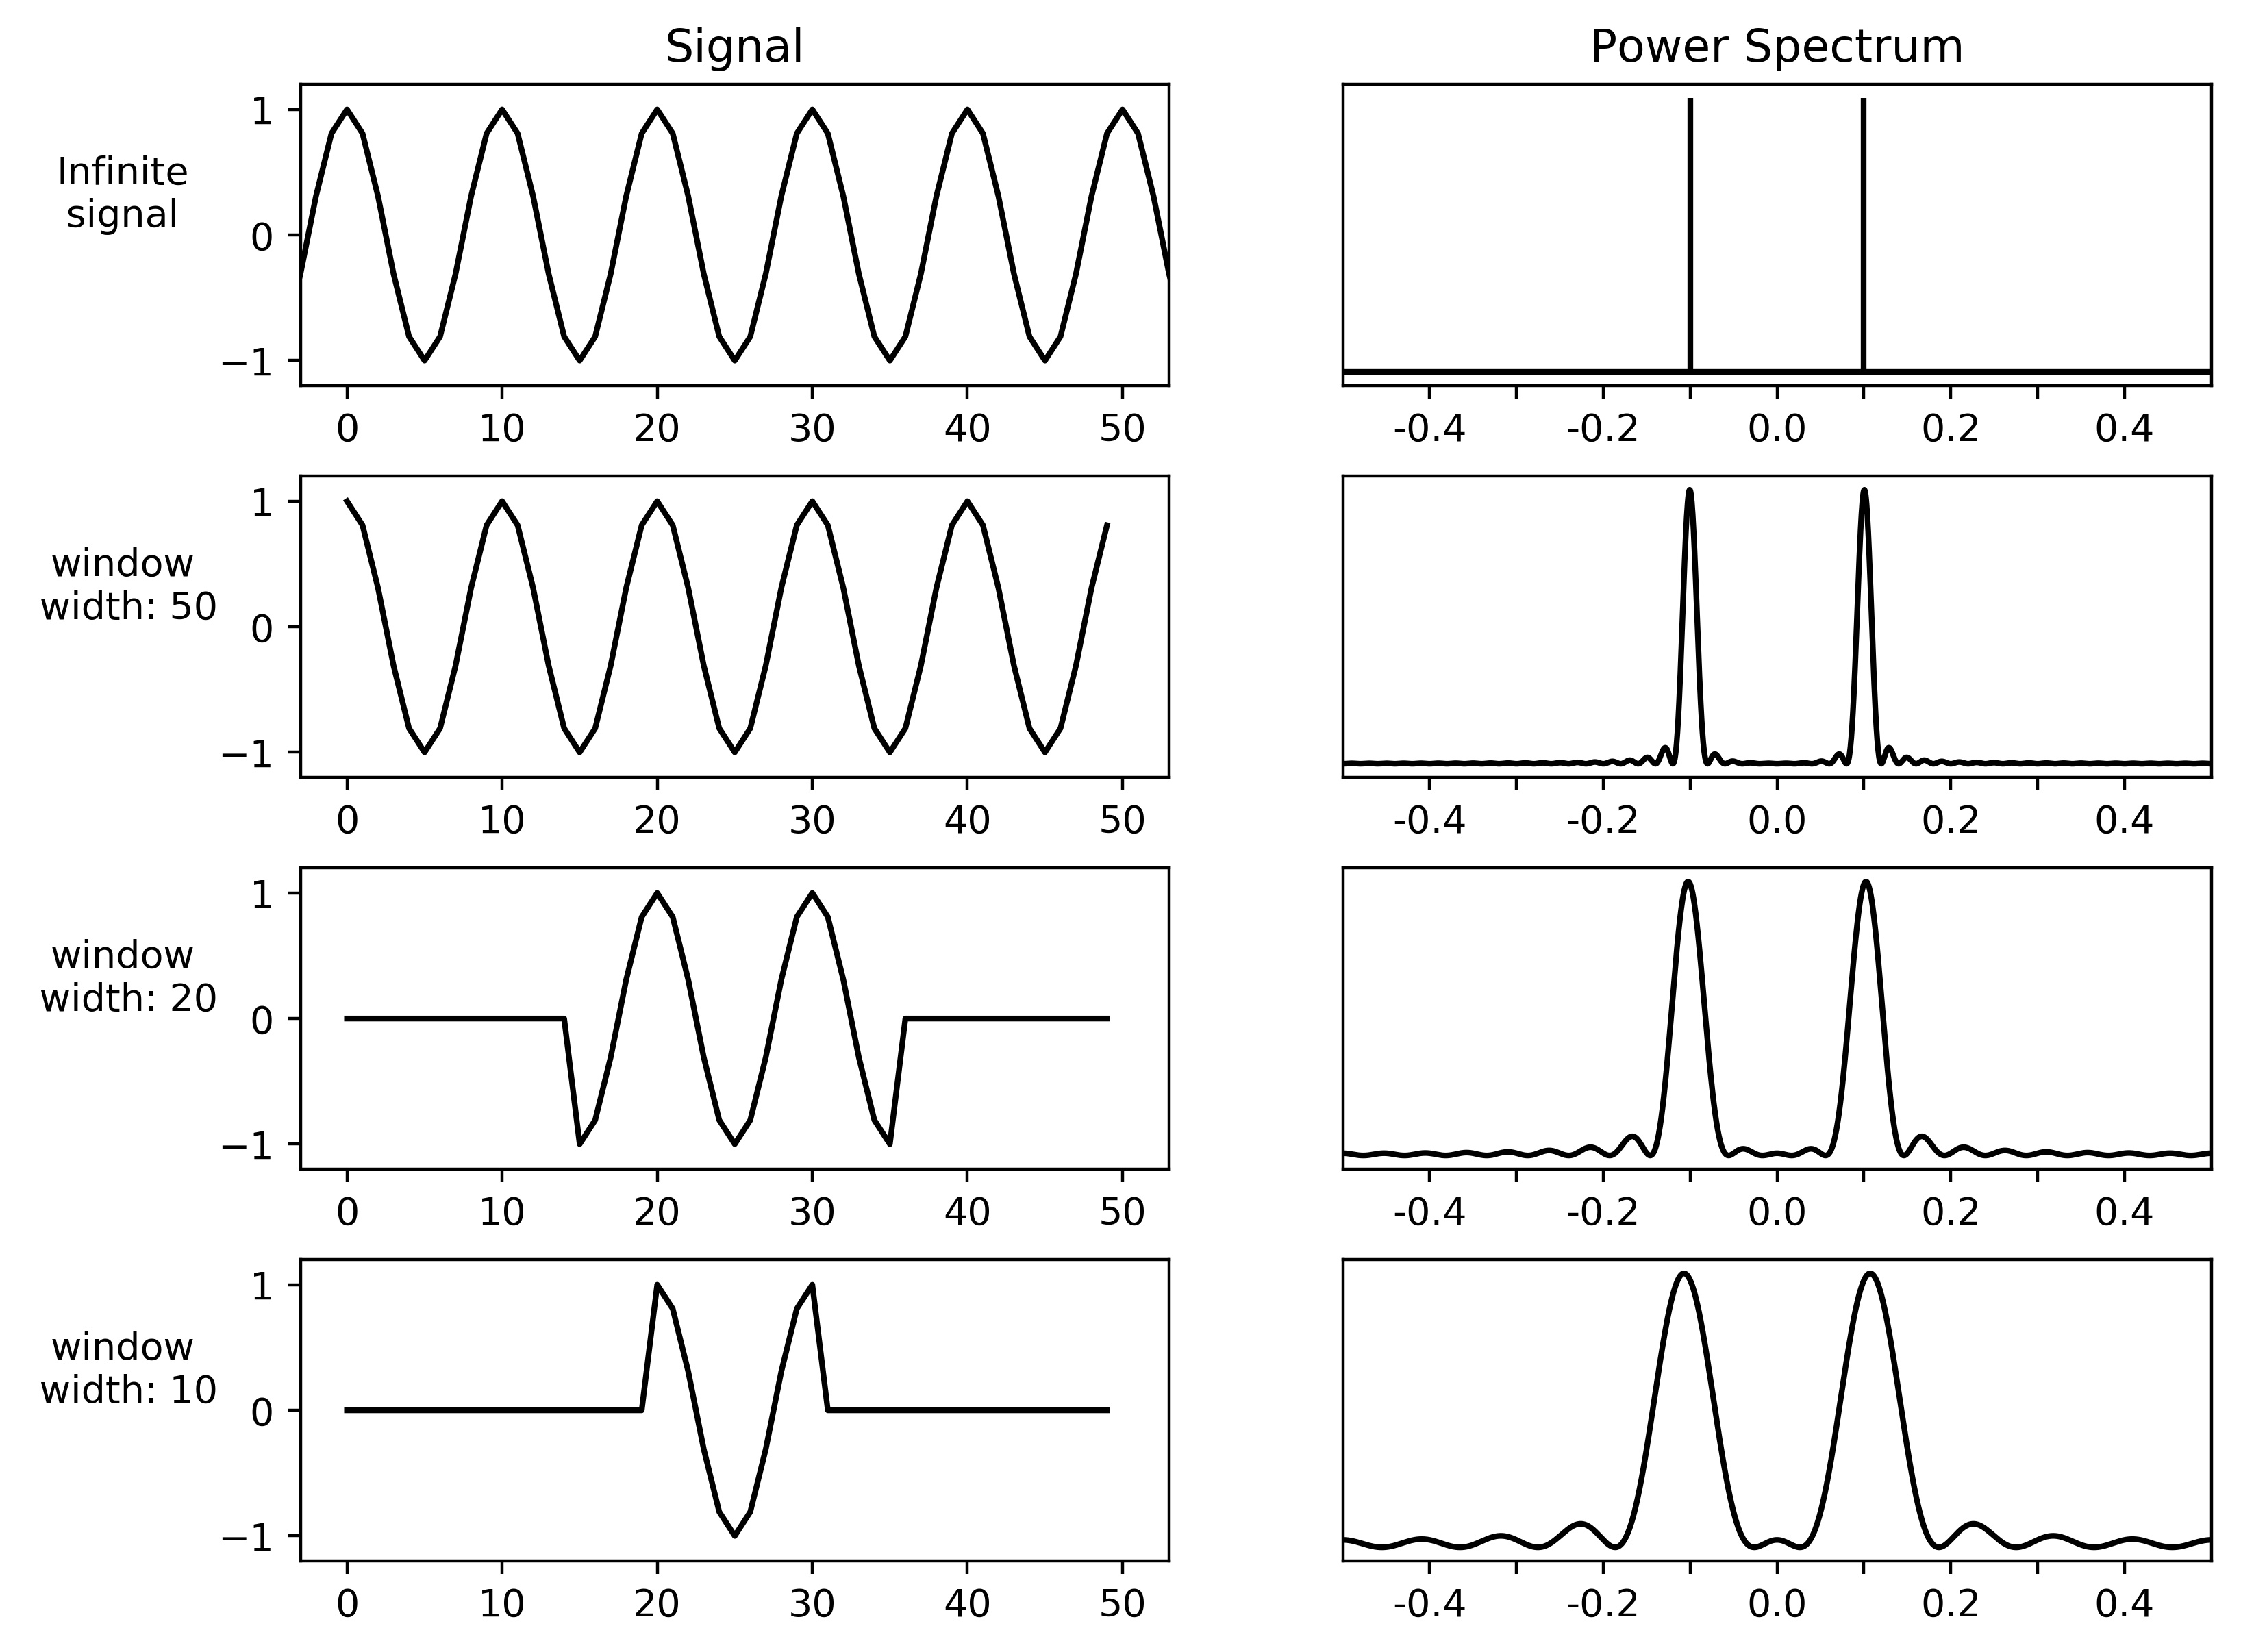
\includegraphics{Figuras/fig1.jpg}}
	\end{center}
	\vspace{1mm}	% acrescentar o espaçamento vertical apropriado entre a borda inferior da figura e a legenda ou a fonte quando não há legenda (o valor pode ser negativo para subir)
	\legenda{Efeitos do tamanho da janela de observação sobre o espectro de potência de um sinal. No topo à esquerda o sinal está representado por uma função analítica que se estende infinitamente, cuja transformada de Fourier (topo à direita) é a função delta sobre a frequência do sinal (no caso, 0.1). Abaixo estão sinais com janelas de observação diferentes e seus respectivos espectros. Quanto menor a janela de observação, maior o efeito dos lóbulos laterais sobre a função delta original, o chamado leakage espectral.}	% legenda - para deixar sem legenda usar comando \legenda{} (nunca deve-se comentar o comando \legenda)
	\label{fig:window}
	%\FONTE{\url{https://omniweb.gsfc.nasa.gov/form/dx1.html}.}	% fonte consultada (elemento obrigatório, mesmo que seja produção do próprio autor)
\end{figure}

\begin{figure}[ht!]
	\caption{Efeitos do sampling rate.}
	\vspace{1mm}	% acrescentar o espaçamento vertical apropriado entre o título e a borda superior da figura
	\begin{center}
		\resizebox{15cm}{!}{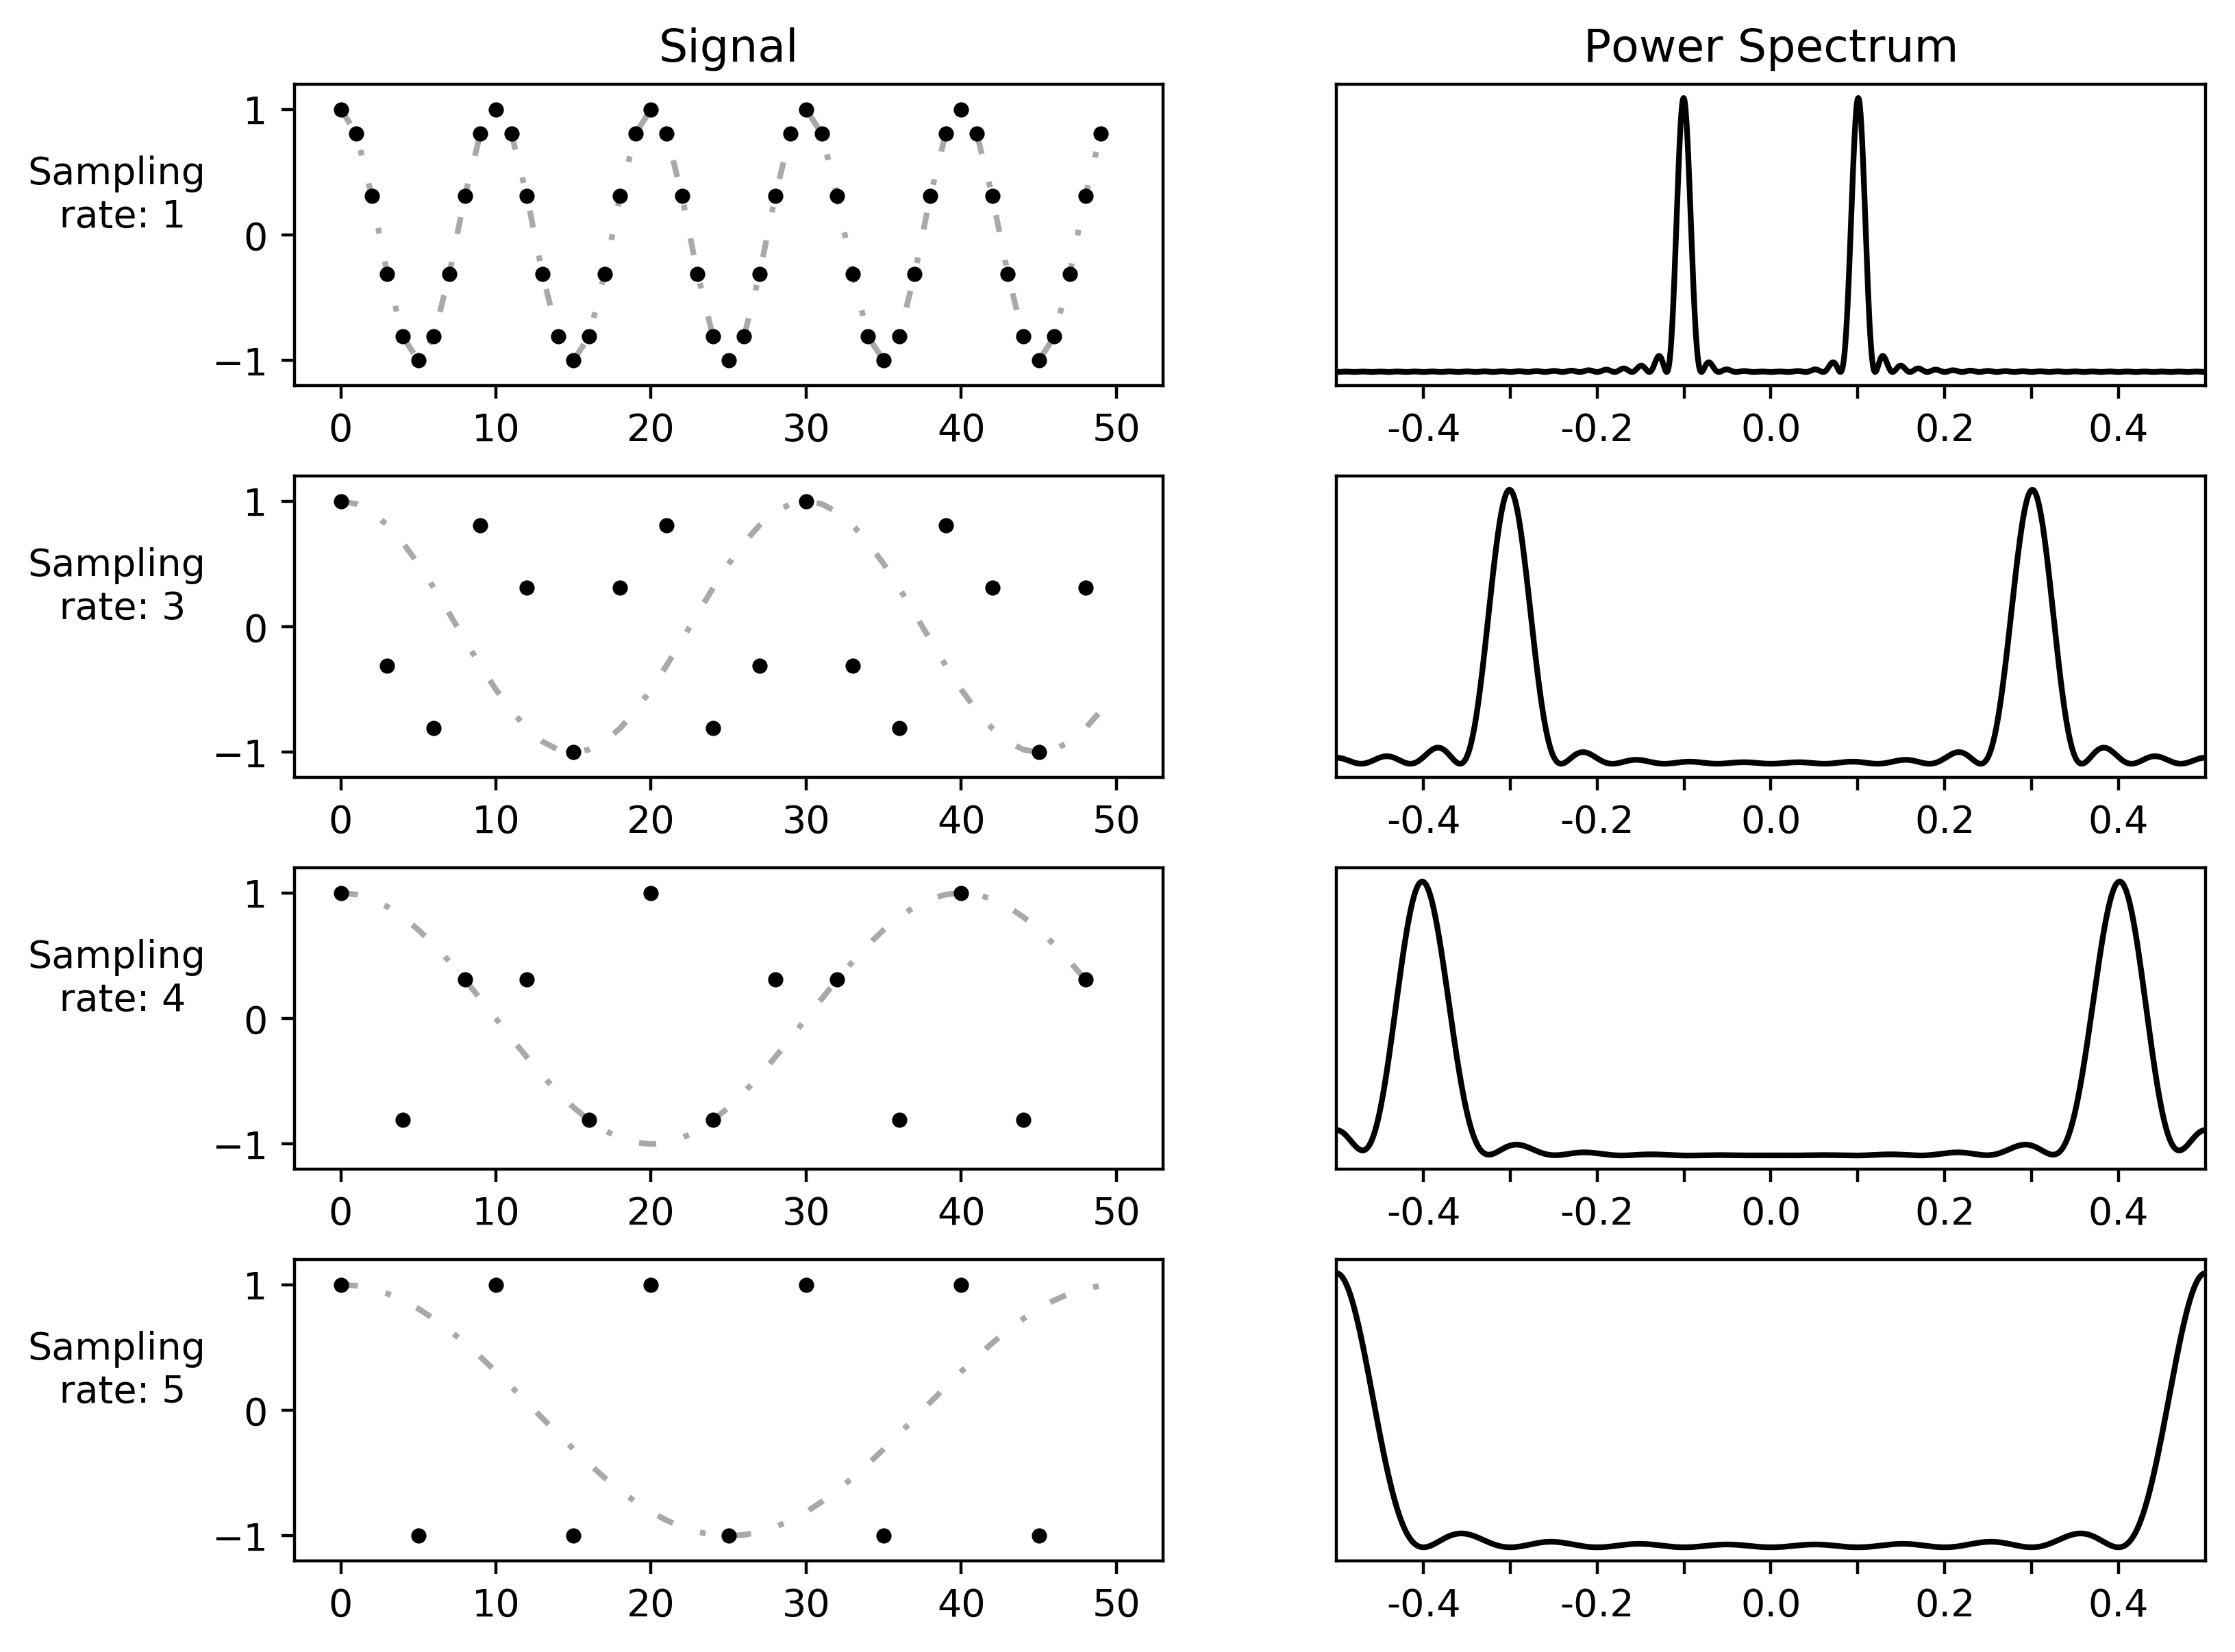
\includegraphics{Figuras/fig2.jpg}}
	\end{center}
	\vspace{1mm}	% acrescentar o espaçamento vertical apropriado entre a borda inferior da figura e a legenda ou a fonte quando não há legenda (o valor pode ser negativo para subir)
	\legenda{Efeitos do sampling rate sobre o espectro de potência de um sinal. No topo, um sinal com um sampling rate igual a um (que corresponde ao sinal com janela de tamanho 50 na Figura \ref{fig:window}). Abaixo, o mesmo sinal sob diferentes sampling rates e seus respectivos espectros. A linha em cinza claro ilustra o sinal falsamente identificado, tanto pelo nosso cérebro quanto pela FFT, conforme indicado nos seus espectros de potência à direita. Fica evidente que para diferentes taxas, diferentes aliases do sinal original são gerados, de modo que a transformada inversa retornaria um sinal totalmente diferentes do original.} % 	% legenda - para deixar sem legenda usar comando \legenda{} (nunca deve-se comentar o comando \legenda)
	\label{fig:sampling}
	%\FONTE{\url{https://omniweb.gsfc.nasa.gov/form/dx1.html}.}	% fonte consultada (elemento obrigatório, mesmo que seja produção do próprio autor)
\end{figure}

Os lóbulos laterais (leakage spectral) são um artefato devido ao intervalo de observação ser finito. As falsas frequências (aliasing) é uma artefato que surge da natureza do sampling. Sabemos que nossos dados de fluxo solar F10.7 são finitos no tempo e apresentam um sampling rate uniforme e satisfatório para gerar bons espectros via FFT, conforme explicitado em \citeonline{Leo}. Mas qual seria o efeito de sampling não uniforme sobre o sinal das figuras anteriores? A Figura 3 ilustra dois cenários de ausência de dados e seus respectivos espectros. Fica evidente a incrível irregularidade do espectro de potência resultante da FFT devido a um espaçamento desigual da amostragem do sinal. 

\begin{figure}[ht!]
	\caption{Efeitos do sampling não uniforme.}
	\vspace{1mm}	% acrescentar o espaçamento vertical apropriado entre o título e a borda superior da figura
	\begin{center}
		\resizebox{15cm}{!}{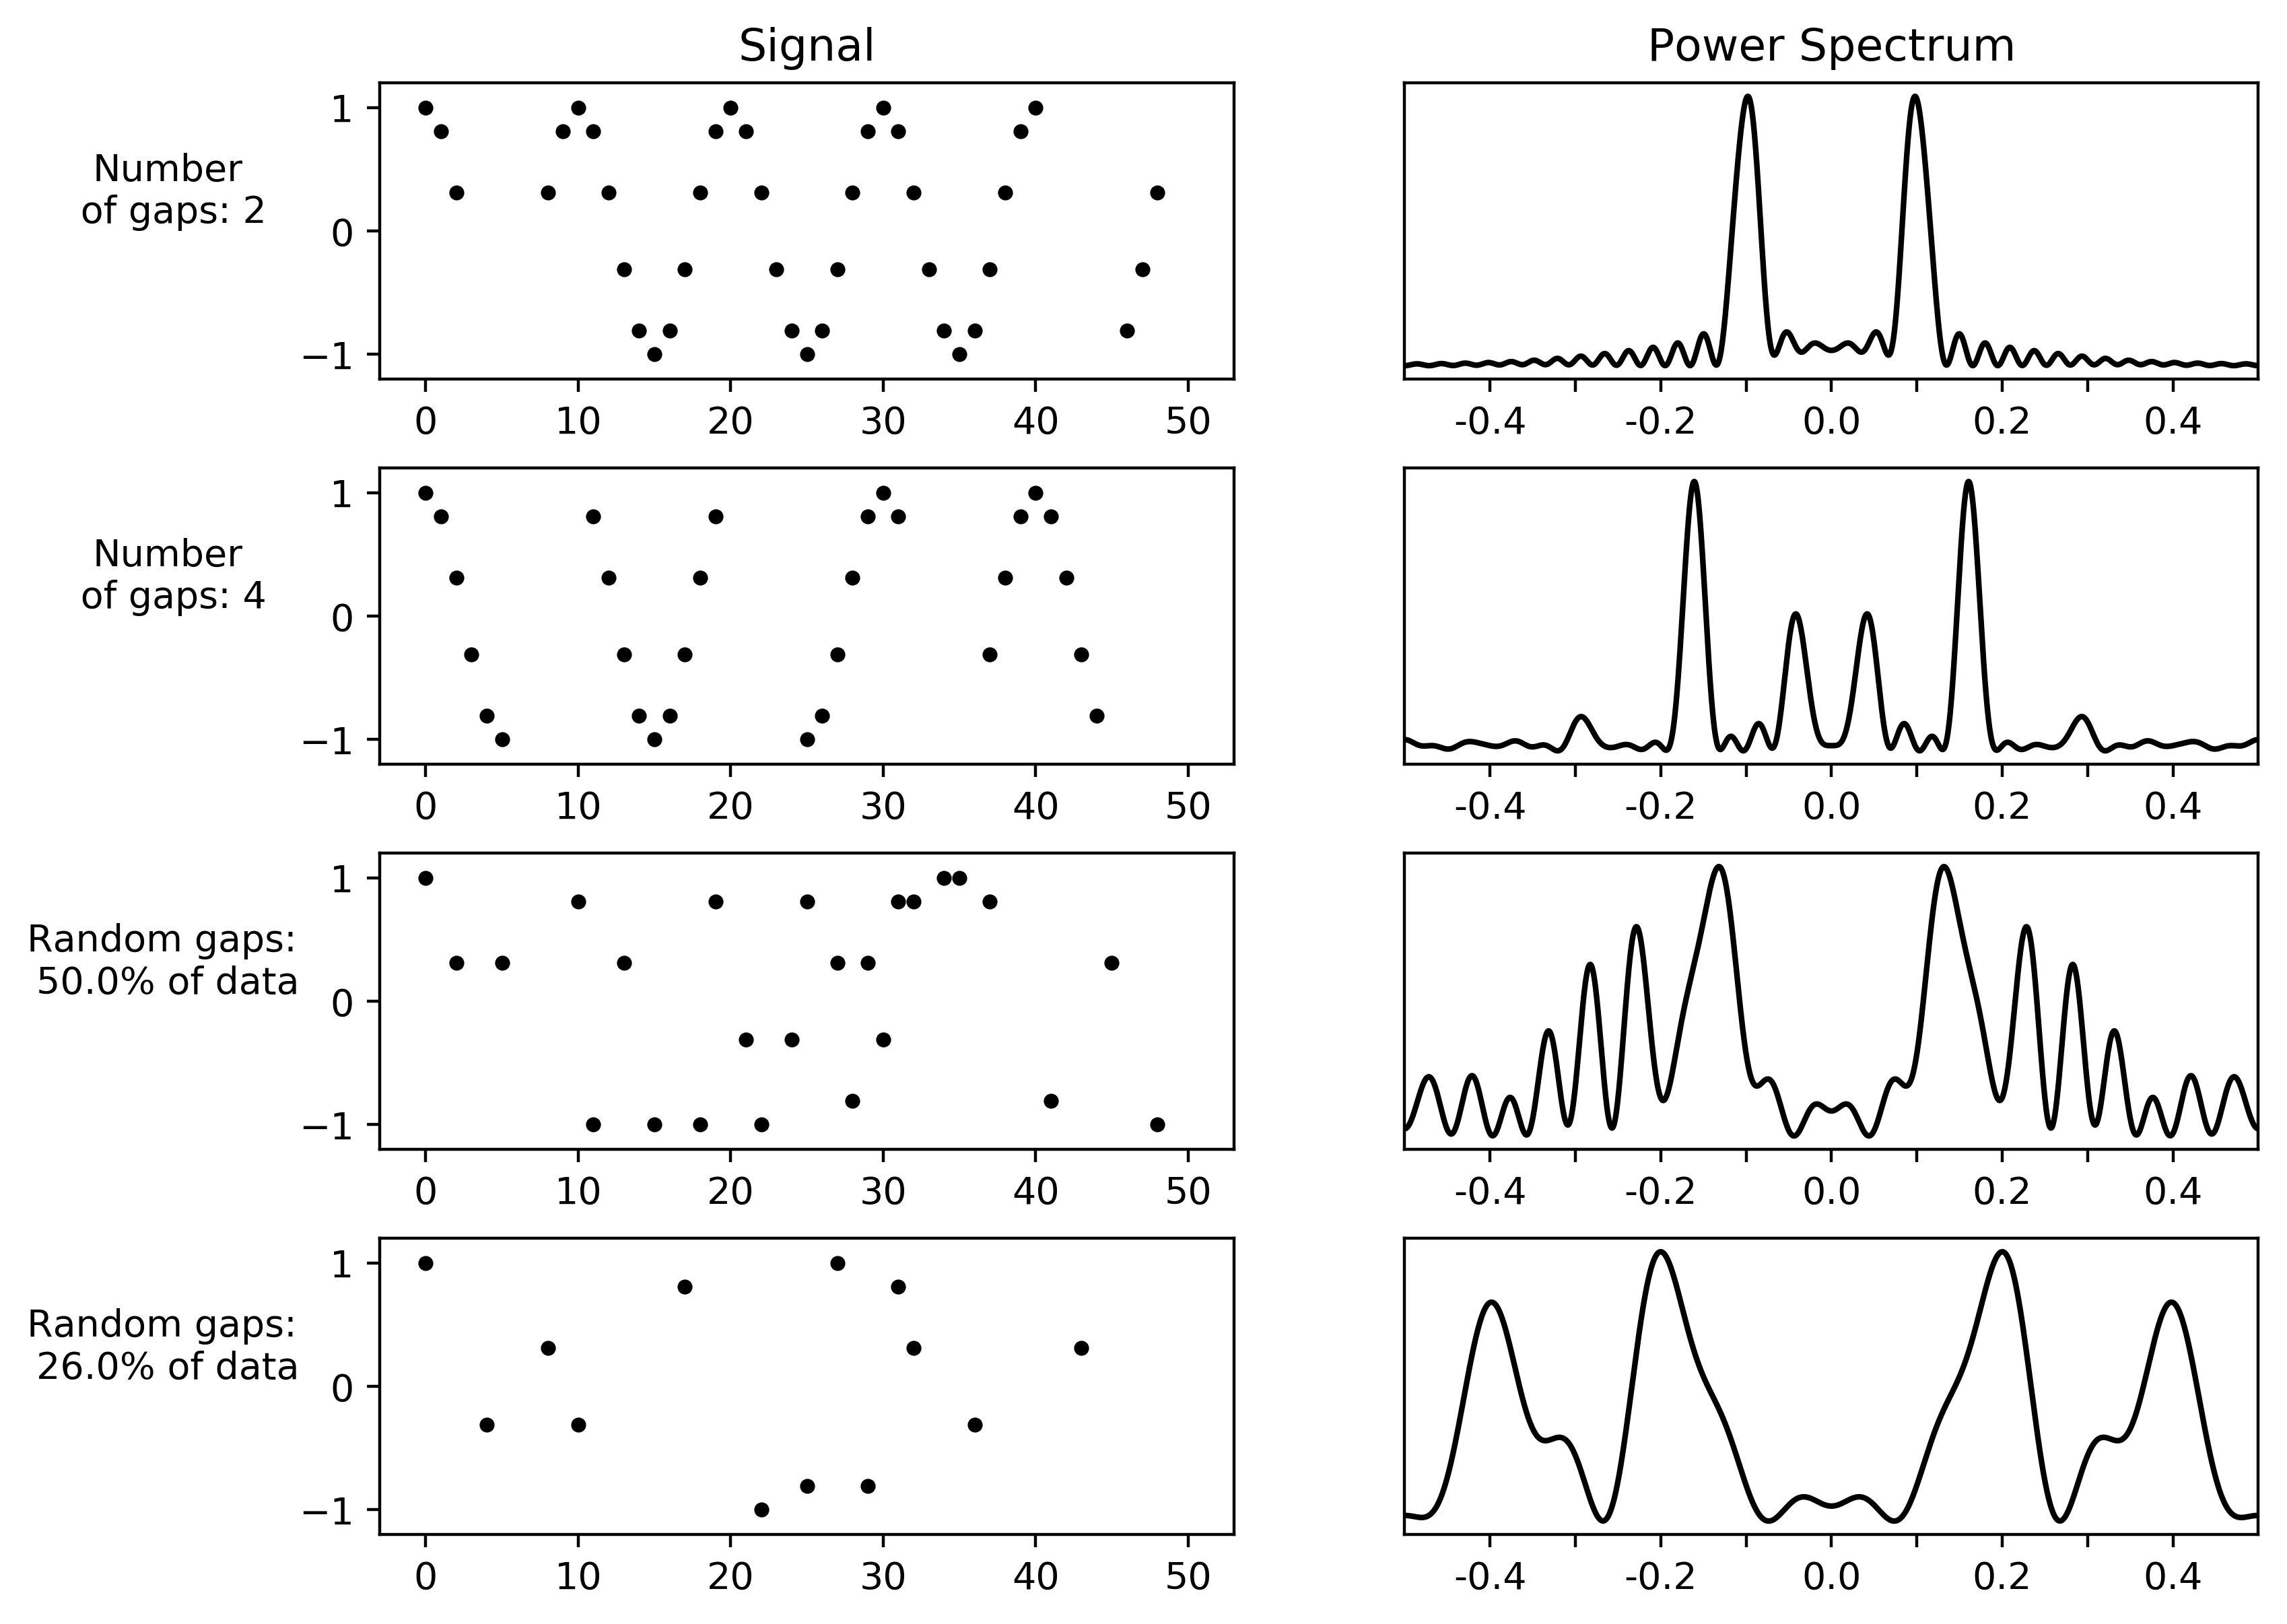
\includegraphics{Figuras/fig3.jpg}}
	\end{center}
	\vspace{1mm}	% acrescentar o espaçamento vertical apropriado entre a borda inferior da figura e a legenda ou a fonte quando não há legenda (o valor pode ser negativo para subir)
	\legenda{Efeitos do sampling não uniforme sobre o espectro de potência de um sinal. No topo, o sinal do topo da Figura \ref{fig:window} se apresenta com dois gaps (intervalos) aleatórios sem dados. Abaixo deste, o mesmo sinal com quatro gaps aleatoriamente posicionados. Os dois últimos sinais representam um cenário com remoção aleatória de dados, um permanecendo com 50\% dos dados e o outro com 26\% apenas. Somente o espectro de potência do primeiro sinal (topo à direita) possui um pico consistente (posicionado na frequência esperada de 0.1).}	% legenda - para deixar sem legenda usar comando \legenda{} (nunca deve-se comentar o comando \legenda)
	\label{fig:uneven}
	%\FONTE{\url{https://omniweb.gsfc.nasa.gov/form/dx1.html}.}	% fonte consultada (elemento obrigatório, mesmo que seja produção do próprio autor)
\end{figure}


\section{Periodograma de Lomb-Scargle}

O periodograma de Lomb-Scargle é a principal ferramenta para análise de séries temporais com amostragem desigual. Ele pertence a um grupo de ferramentas de análise espectral que explora o método de mínimos quadrados, estimando frequências do sinal a partir de testes sobre frequências pré-determinadas com o fim de ajustar funções senoidais aos dados. O periodograma de Lomb-Scargle é dos métodos de análise espectral por mínimos quadrados desenvolvido por \citeonline{lomb1976least} com posterior contribuição de \citeonline{scargle1982studies}. Ele está disponível no pacote \texttt{astropy} (com complexidade $O[NlogN]$) através da classe \texttt{LombScargle}, e pode ser facilmente implementado:

\vspace{-2mm}
\begin{lstlisting}[language=python,style=mystyle2]
from astropy.timeseries import LombScargle
frequency, power = LombScargle(t, f).autopower()
\end{lstlisting}

No exemplo acima, o periodograma de Lomb-Scargle foi aplicado a um sinal \texttt{f} amostrado em tempos irregulares conforme o array \texttt{t}, gerando um array com as frequências testadas (\texttt{frequency}) e o periodograma resultante (\texttt{power}). O método \texttt{autopower()} aplica uma heurística para selecionar frequências adequadas ao teste de mínimos quadrados. Pode-se ajustar essa mesma heurística para testar frequências mais altas e com maior resolução através da palavra-chave \texttt{nyquist\_factor}. O valor de dois foi empregado nas análises deste trabalho. Além disso, é possível passar como um terceiro input a incerteza dos dados, pois a classe \texttt{LombScargle} é capaz de considerar incertezas em seus cálculos (assume-se incerteza gaussiana). O sinusoide de melhor ajuste pode ser computado a partir do método \texttt{model()}. O output da classe \texttt{LombScargle} é adimensional e por padrão normalizado (seus valores estão entre 0 e 1). Alguns desses recursos são explorados na próxima seção.

%\begin{lstlisting}[language=python,style=mystyle2]
%frequency,power=LombScargle(t,y,dy).autopower(nyquist_factor=10)
%\end{lstlisting}

%A seção a seguir apresenta o resultado da implementação desta classe sobre diferentes cenários de aquisição aleatória dos dados de fluxo solar F10.7.  

 %% 3o capítulo

%%%%%%%%%%%%%%%%%%%%%%%%%%%%%%%%%%%%%%%%%%%%%%%%%%%%%%%%%%%%%%%%%%%%%%%%%%%%%%%
%\vspace{-2mm}
\chapter{RESULTADOS E DISCUSSÃO}

A presente seção apresenta e discute o resultado da aplicação da classe \texttt{LombScarbgle} do pacote \texttt{astropy} sobre os dados do fluxo solar F10.7. Mas antes, a Figura \ref{fig:original365} exibe o espectro de potência dos dados de média diárias do índice F10.7. Ele foi obtido via FFT conforme explicitado em \citeonline{Leo}. % aos três conjuntos de dados originais: dados de médias diárias, médias de 27 dias e médias anuais do índice solar F10.7 (Figura \ref{fig:original365}, \ref{fig:original12} e \ref{fig:original1}, respectivamente). O espectro de potência foi obtido conforme explicitado em \citeonline{Leo}. 

\vspace{-8mm}
\begin{figure}[ht!]
	\caption{Espectro de potência dos dados originais (média diária).}
	\vspace{1mm}	% acrescentar o espaçamento vertical apropriado entre o título e a borda superior da figura
	\begin{center}
		\resizebox{.7\textwidth}{!}{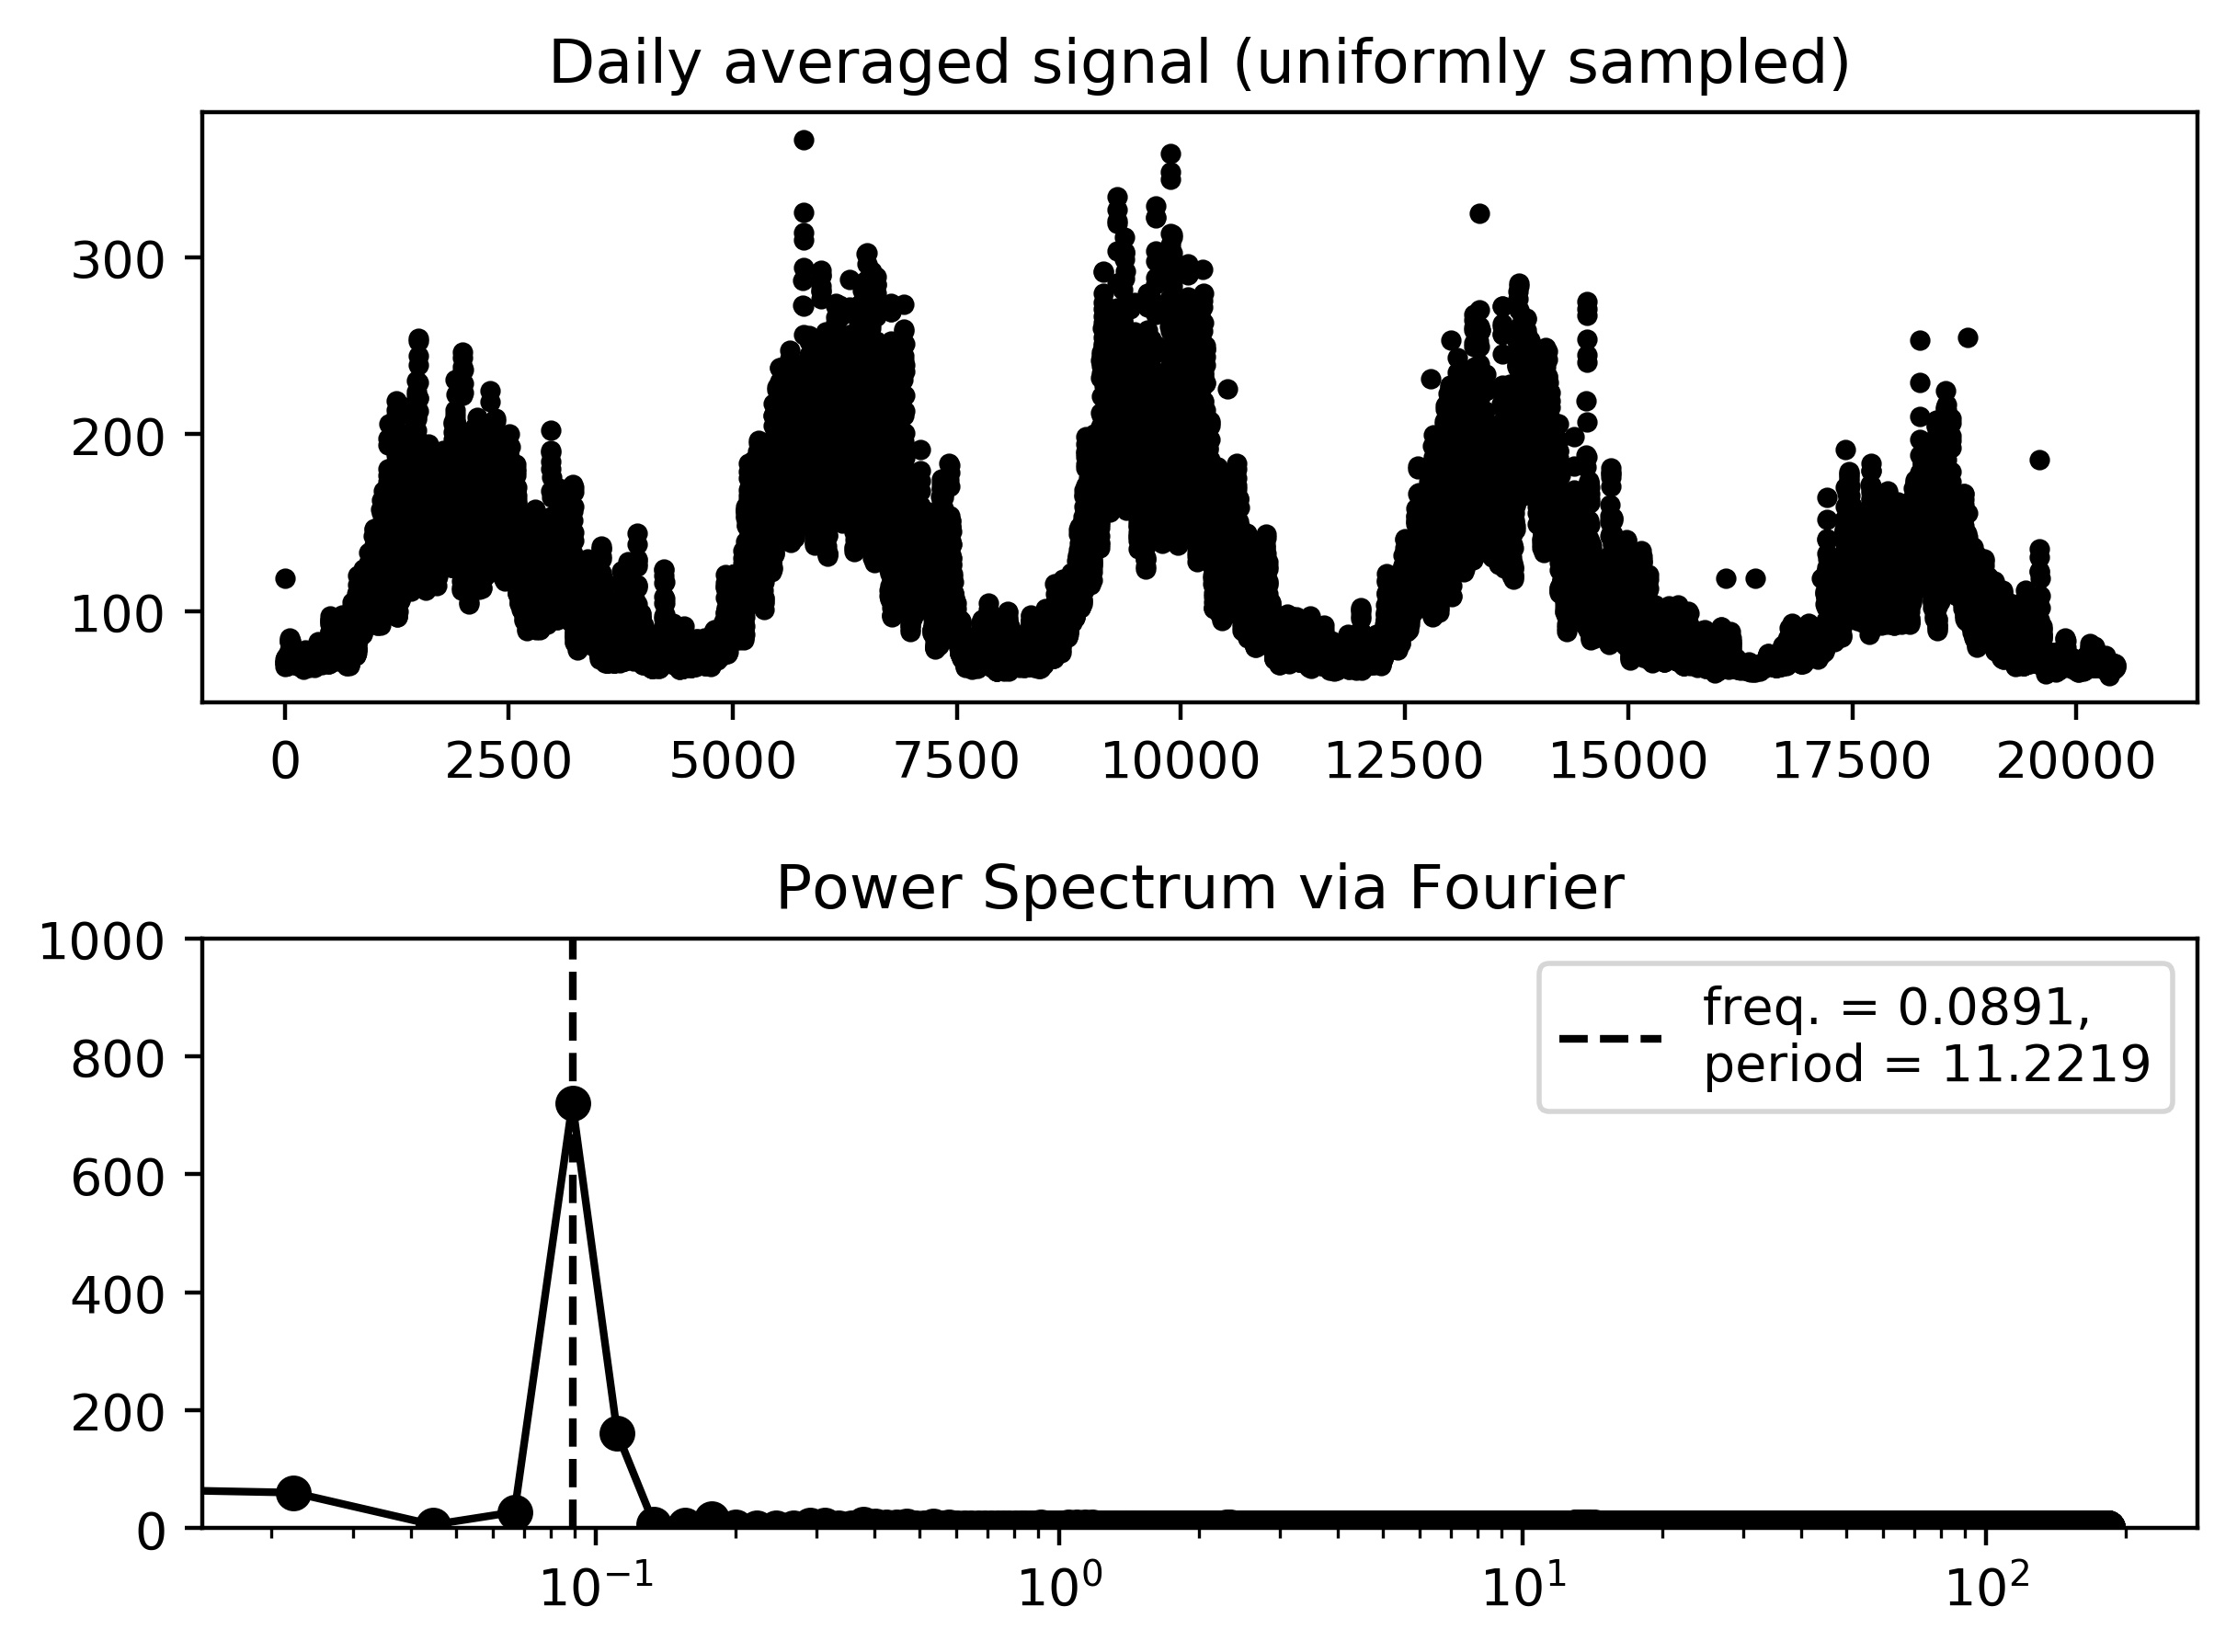
\includegraphics{Figuras/original_365.jpg}}
	\end{center}
	\vspace{-1mm}	% acrescentar o espaçamento vertical apropriado entre a borda inferior da figura e a legenda ou a fonte quando não há legenda (o valor pode ser negativo para subir)
	\legenda{Espectro de potência via FFT das médias diárias do índice  solar F10.7. Com amostragem uniforme, longa janela de observação e sampling rate satisfatório, a técnica do espectro de Fourier via algoritmos de FFT é um método robusto e amplamente empregado.}	% legenda - para deixar sem legenda usar comando \legenda{} (nunca deve-se comentar o comando \legenda)
	\label{fig:original365}
	%\FONTE{\url{https://omniweb.gsfc.nasa.gov/form/dx1.html}.}	% fonte consultada (elemento obrigatório, mesmo que seja produção do próprio autor)
\end{figure}

%\begin{figure}[ht!]
%	\caption{Espectro de potência dos dados originais (média de 27 dias).}
%	\vspace{1mm}	% acrescentar o espaçamento vertical apropriado entre o título e a borda superior da figura
%	\begin{center}
%		\resizebox{.8\textwidth}{!}{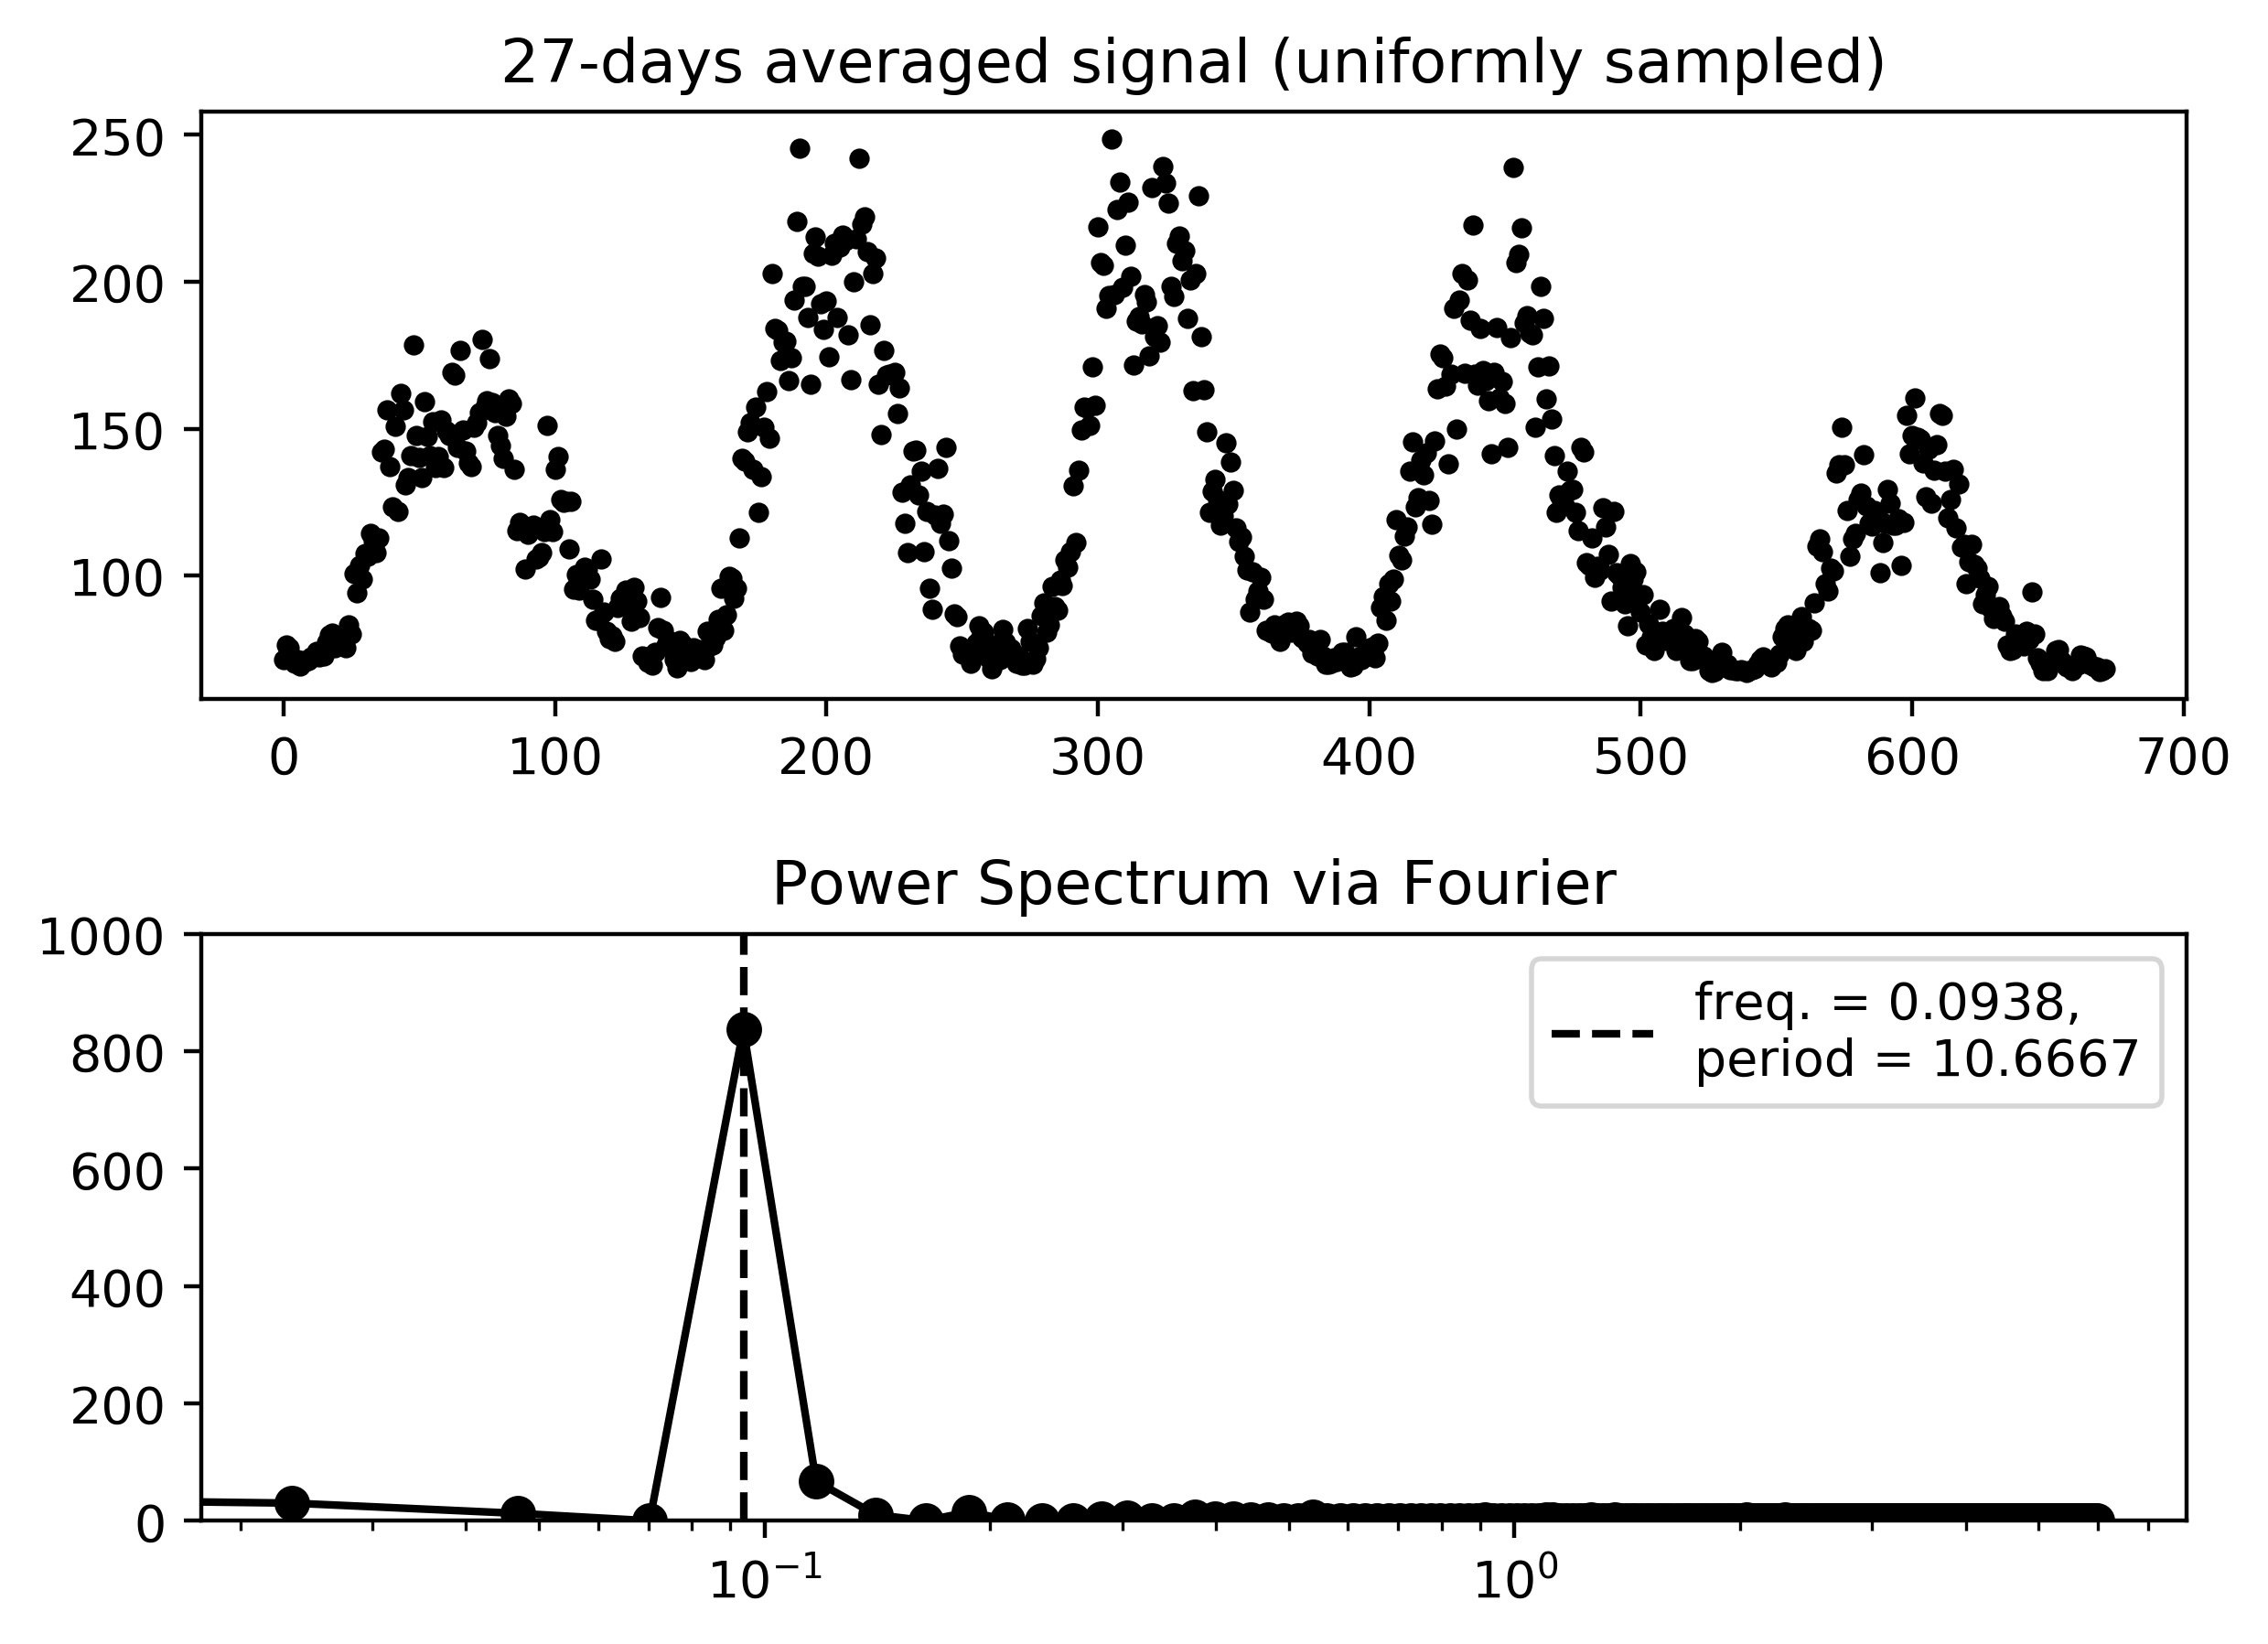
\includegraphics{Figuras/original_12.jpg}}
%	\end{center}
%	\vspace{-1mm}	% acrescentar o espaçamento vertical apropriado entre a borda inferior da figura e a legenda ou a fonte quando não há legenda (o valor pode ser negativo para subir)
%	\legenda{Aplicação do espectro de Fourier sobre as médias de 27 dias do índice  solar F10.7 sob amostragem uniforme. Novamente a análise de Fourier pode ser empregada sem problemas.}	% legenda - para deixar sem legenda usar comando \legenda{} (nunca deve-se comentar o comando \legenda)
%	\label{fig:original12}
	%\FONTE{\url{https://omniweb.gsfc.nasa.gov/form/dx1.html}.}	% fonte consultada (elemento obrigatório, mesmo que seja produção do próprio autor)
%\end{figure}

%\begin{figure}[ht!]
%	\vspace{-20mm}	
%	\caption{Espectro de potência dos dados originais (média anual).}
%	\vspace{1mm}	% acrescentar o espaçamento vertical apropriado entre o título e a borda superior da figura
%	\begin{center}
%		\resizebox{.8\textwidth}{!}{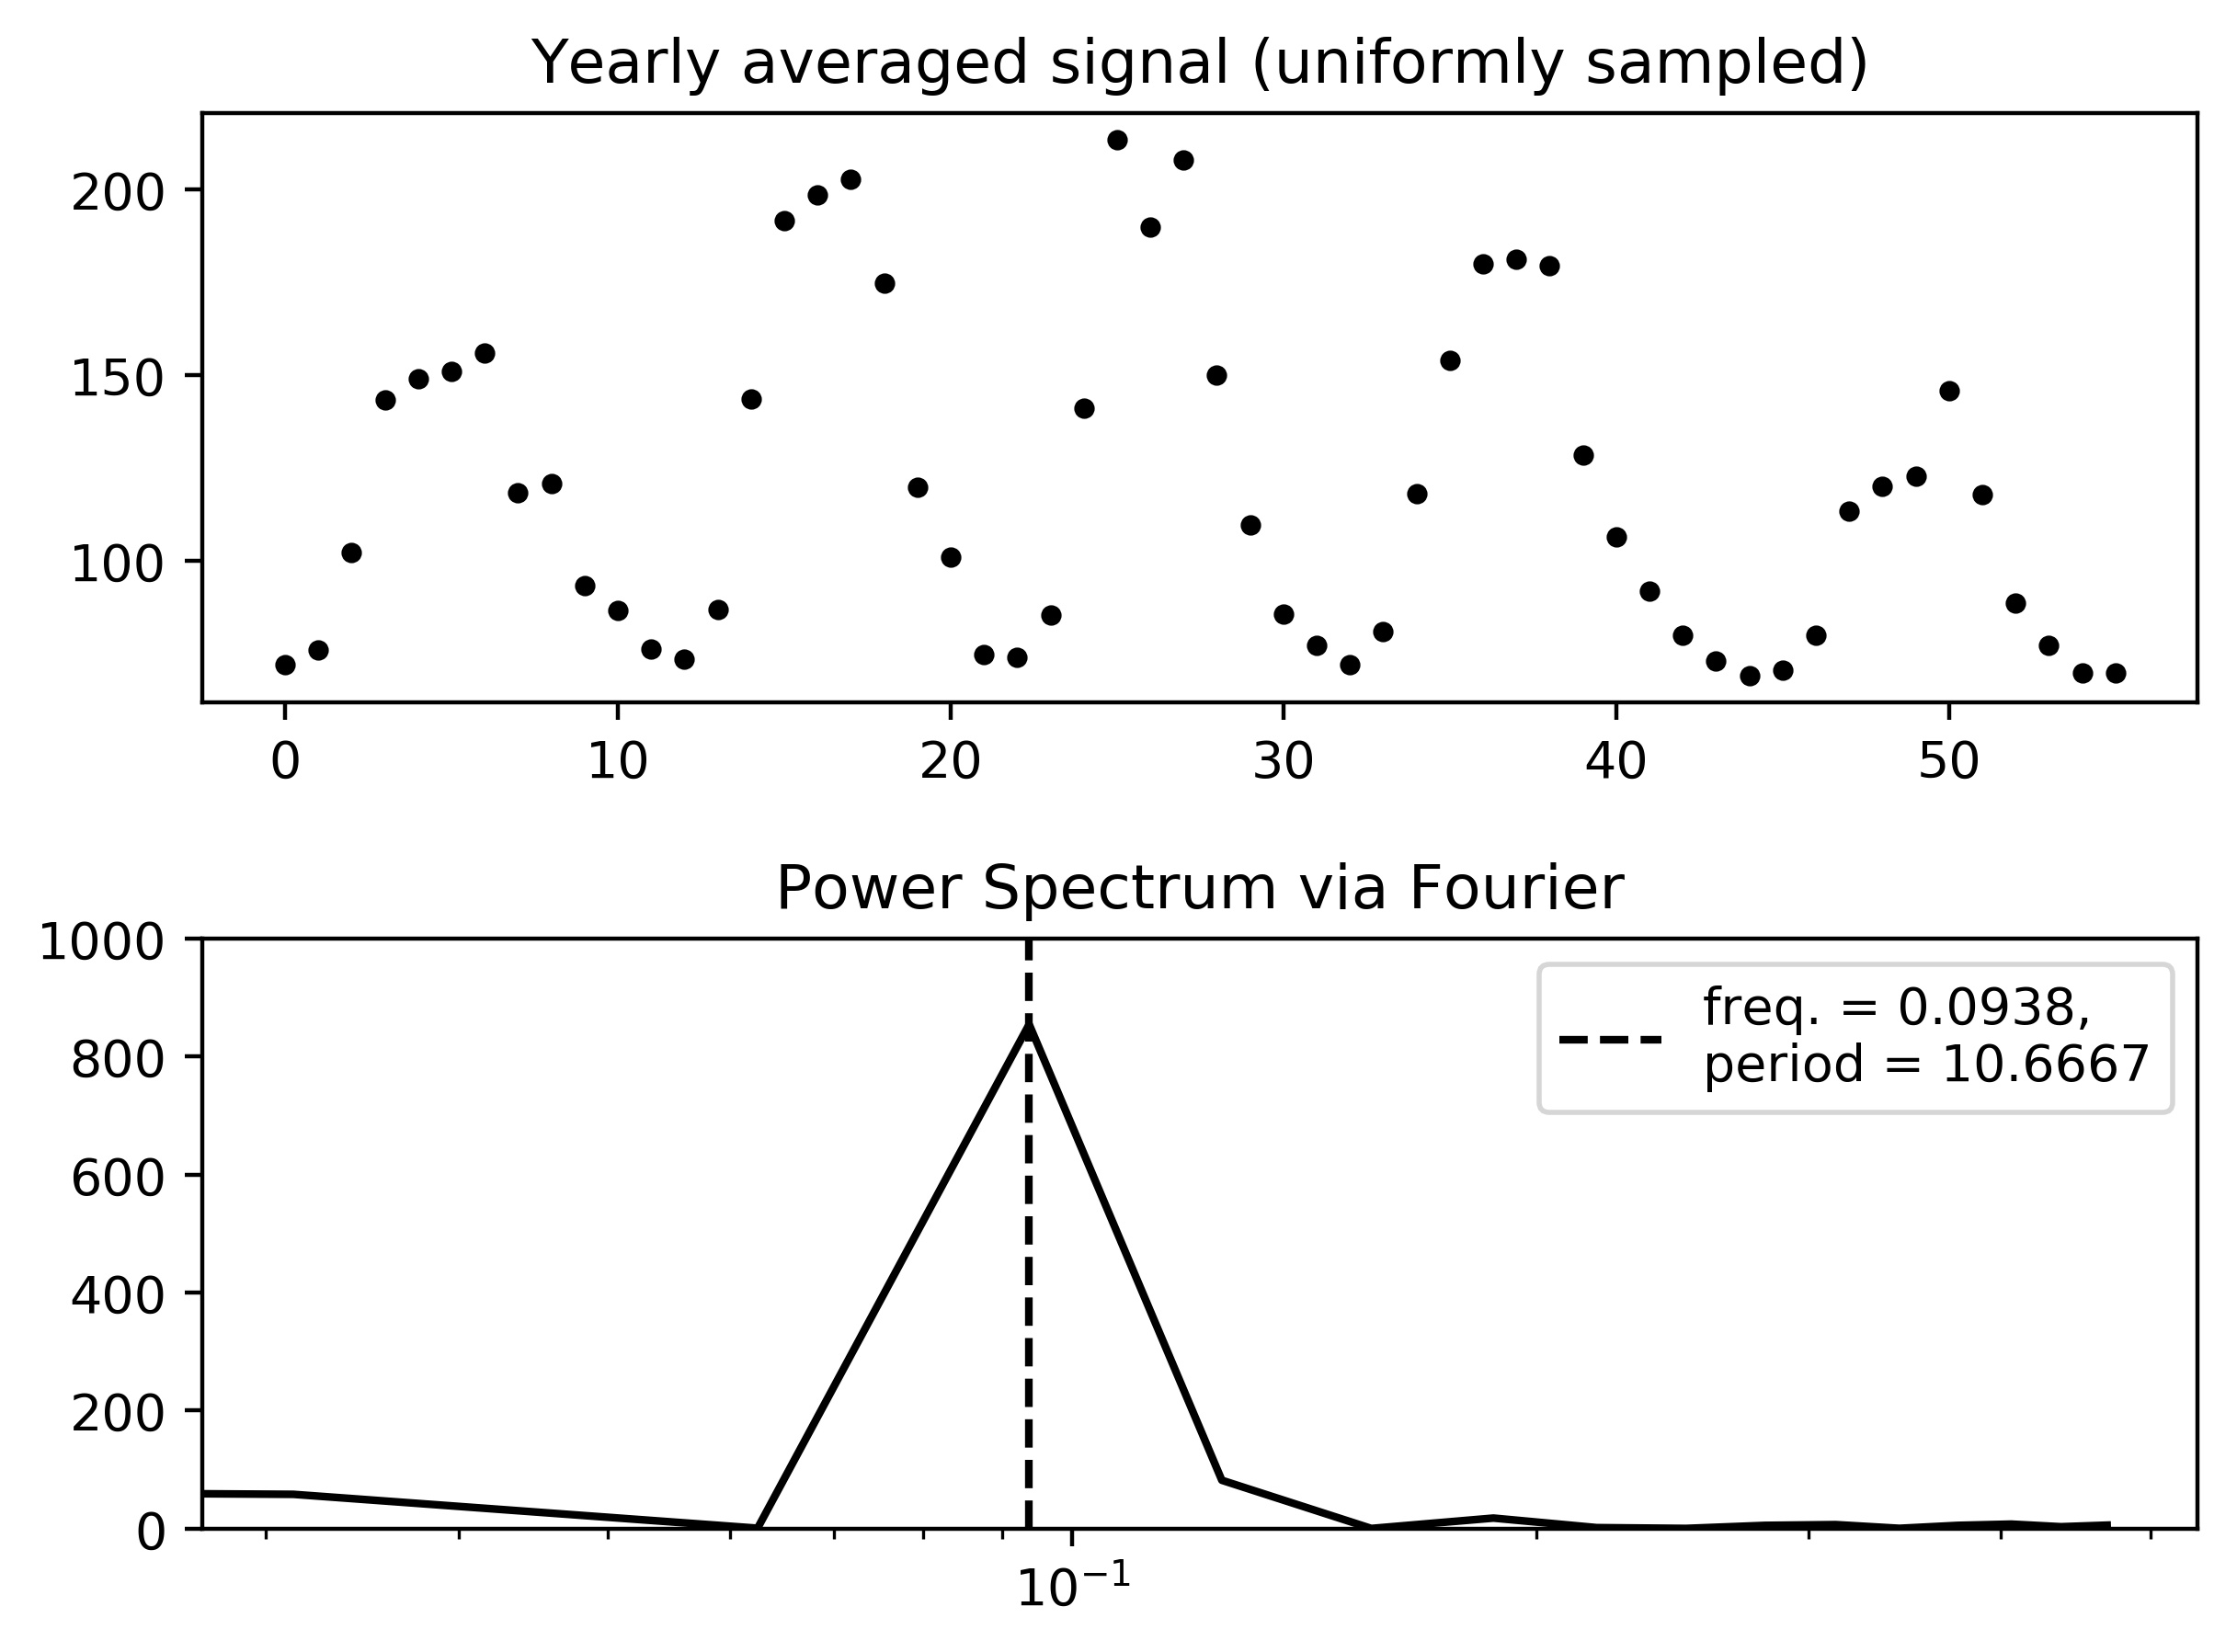
\includegraphics{Figuras/original_1.jpg}}
%	\end{center}
%	\vspace{-1mm}	% acrescentar o espaçamento vertical apropriado entre a borda inferior da figura e a legenda ou a fonte quando não há legenda (o valor pode ser negativo para subir)
%	\legenda{Aplicação do espectro de Fourier sobre as médias anuais do índice  solar F10.7. A amostragem novamente é uniforme, porém com taxa muito inferior à dos demais conjuntos de dados. Ainda assim o espectro de potência via Fourier se mostra uma ferramenta poderosa.}	% legenda - para deixar sem legenda usar comando \legenda{} (nunca deve-se comentar o comando \legenda)
%	\label{fig:original365}
	%\FONTE{\url{https://omniweb.gsfc.nasa.gov/form/dx1.html}.}	% fonte consultada (elemento obrigatório, mesmo que seja produção do próprio autor)
%\end{figure}

\clearpage{}
Nas seções a seguir, os dados de médias diárias do fluxo F10.7 são investigados sob diferentes cenários de amostragem aleatória. O primeiro cenário se baseia em gaps (intervalos) de interrupção na aquisição dos dados. São testados cinco números de gaps diferentes, posicionados aleatoriamente e com o mesmo tamanho. O segundo cenário simula a ausência aleatória dos dados, considerando cinco porcentagens diferentes do tamanho inicial da amostra para exclusão. Em todos os casos o resultado e a performance da classe \texttt{LombScargle} do pacote \texttt{astropy} são discutidos. A heurística da ferramenta foi configurada com \texttt{nyquist\_factor} $=$ 2 durante os testes.

\section{Cenário 1 - diferentes intervalos de observação}

Aqui são apresentados os resultados do periodograma de Lomb-Scargle para o cenário de interrupção de observação com intervalos aleatoriamente posicionados nos dados. Em todos os testes o intervalo tem tamanho fixo e igual a 10\% to tamanho da série total. A seguir são exibidos as figuras referentes às médias diárias do índice F10.7. %Os demais resultados estão disponíveis em LINK DO REPOSITÓRIO.

%\subsection{Médias diárias}

\begin{figure}[ht!]
\vspace{-7mm}	
	\caption{Análise das médias diárias com 4 intervalos.}
	\vspace{1mm}	
	\begin{center}
		\resizebox{.8\textwidth}{!}{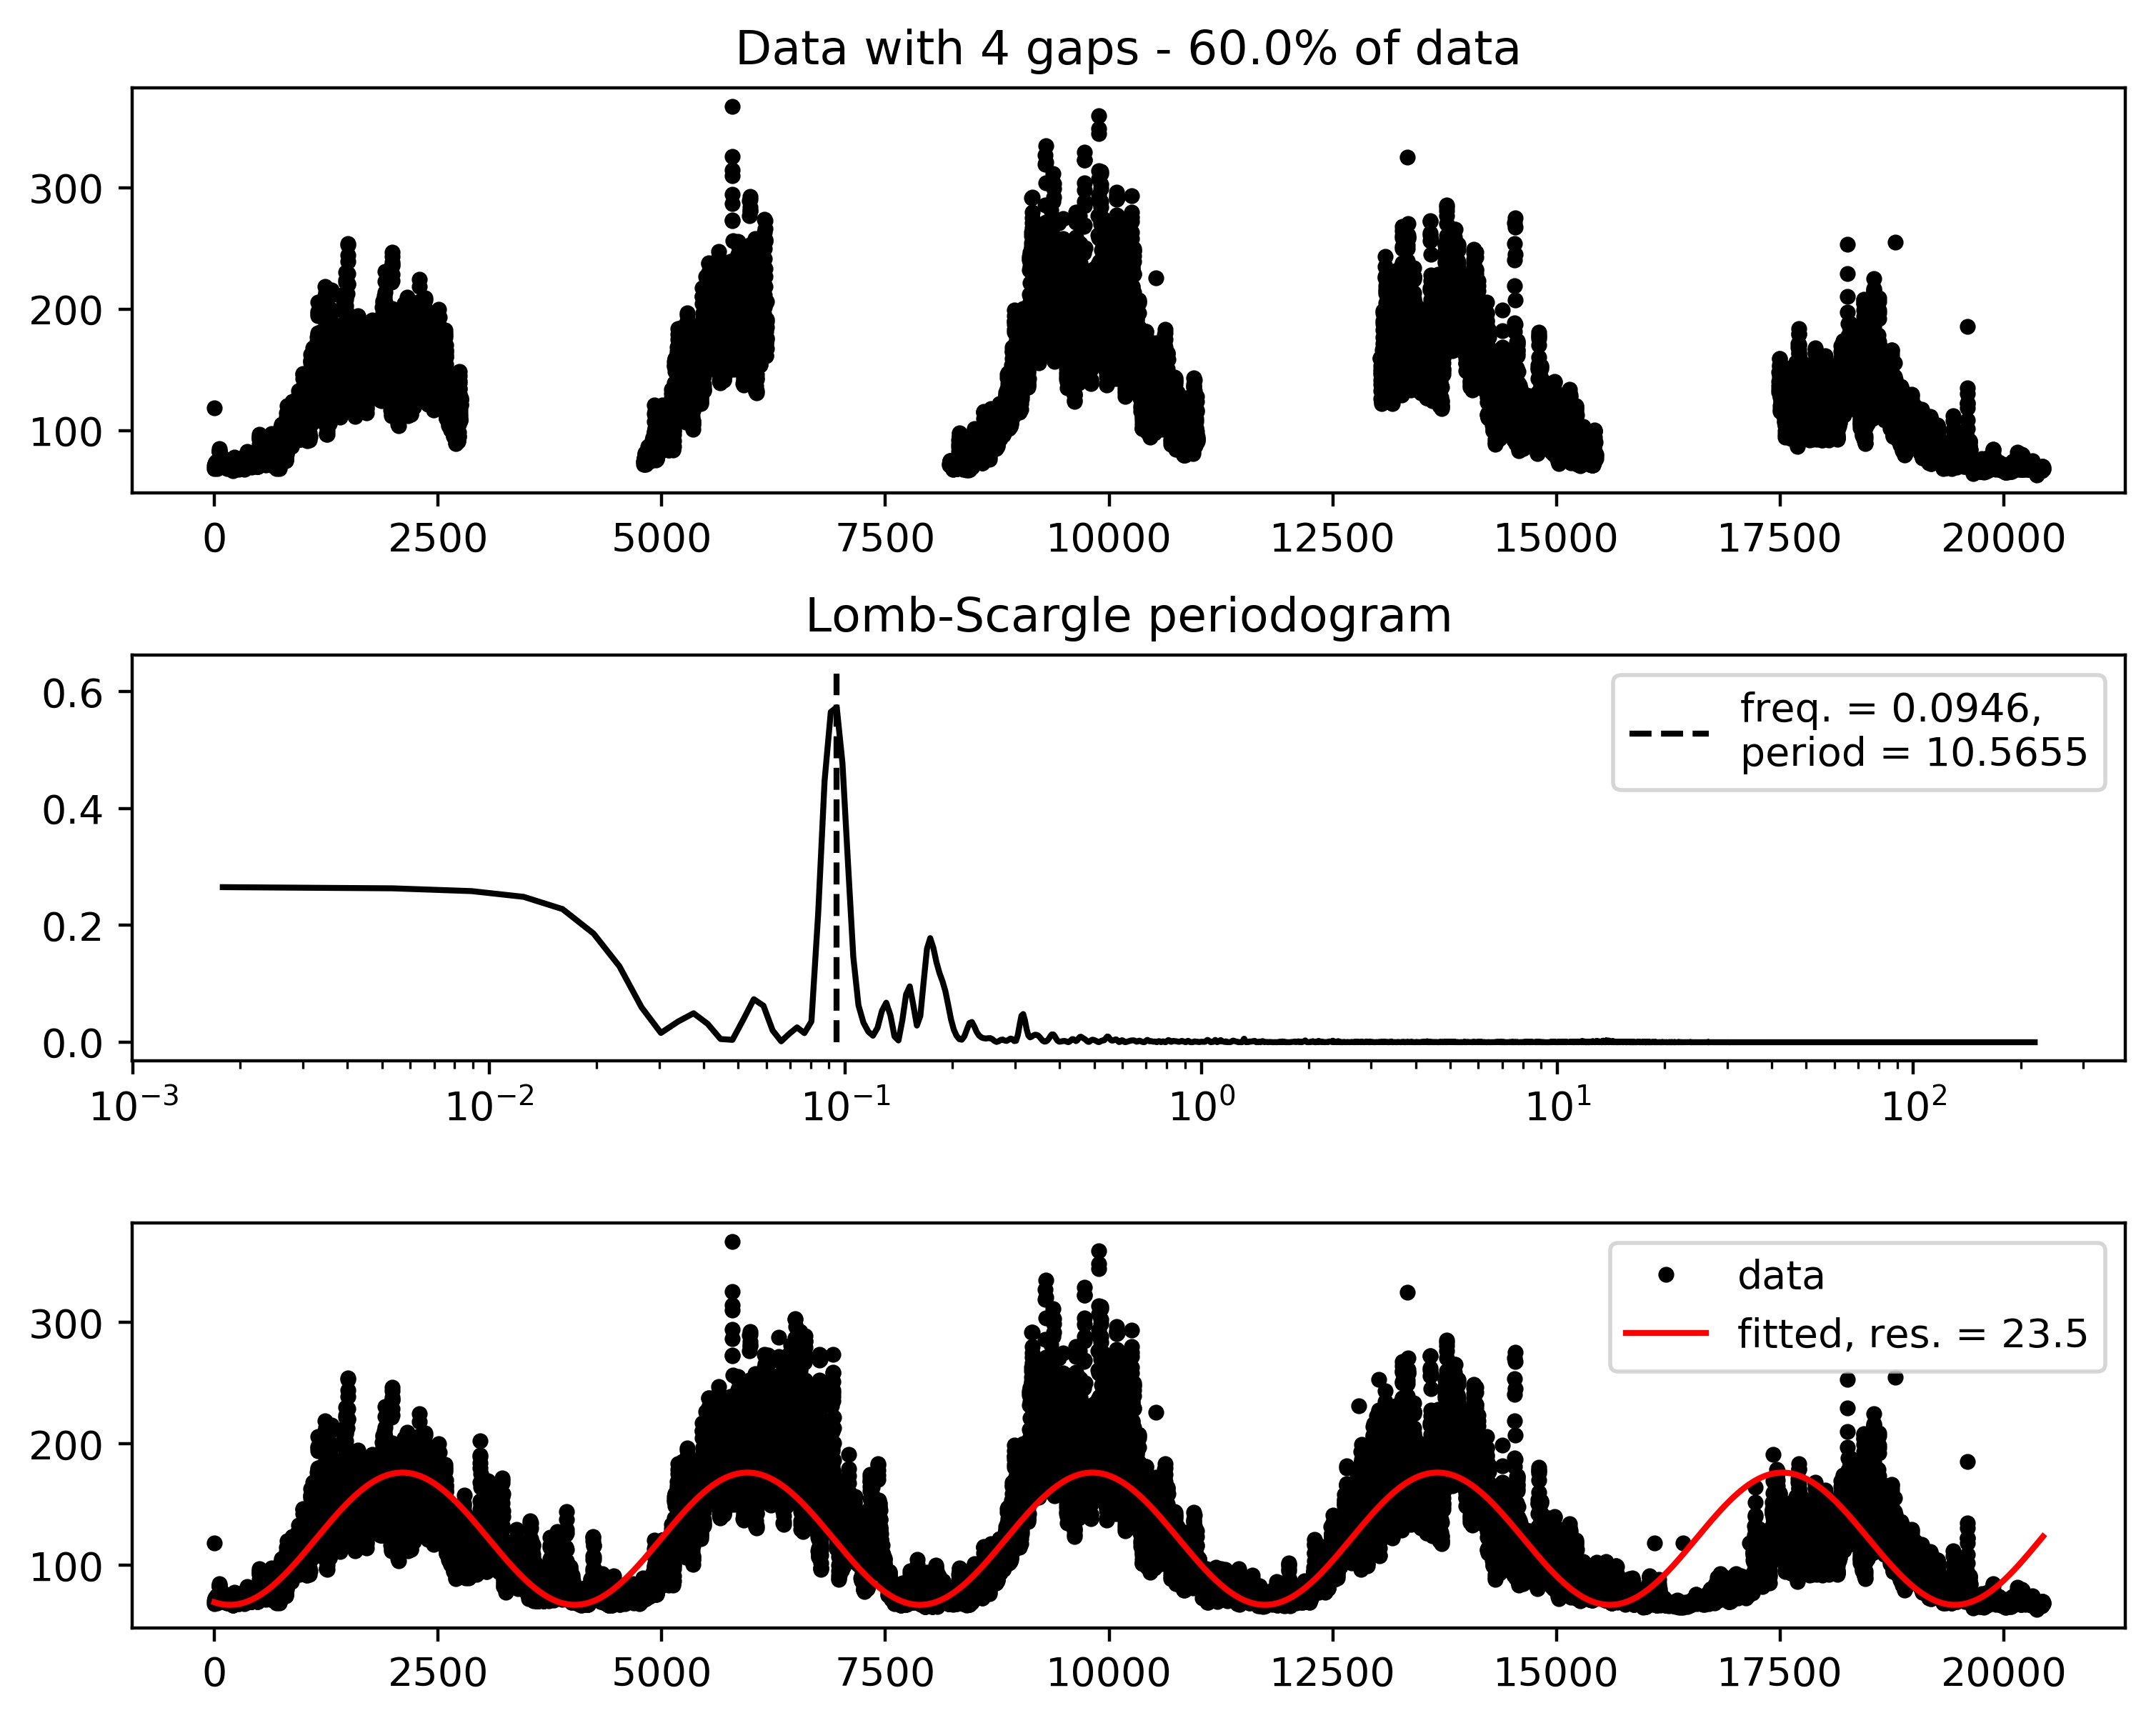
\includegraphics{../scripts/dataset1/periodograms_ny2.0_model2_Ng4.jpg}}
	\end{center}
	\vspace{-1mm}	
	\legenda{Topo: série de médias diárias do fluxo 10.7 com a presença de 4 gaps na obtenção de dados, restando assim 60\% dos dados originais. Meio: periodograma de Lomb-Scargle com indicação da frequência predominante determinada pela localização do pico. Abaixo: em preto a série original, em vermelho a senóide determinada a partir do método \texttt{model()}. O resíduo médio é indicado, quantificando o quanto a função ajustada pelo pacote \texttt{LombScargle} se aproxima da série original.}
	\label{fig:4gaps}
\end{figure}

\begin{figure}[ht!]
\vspace{-10mm}	
	\caption{Análise das médias diárias com 5 intervalos.}
	\vspace{1mm}	
	\begin{center}
		\resizebox{.8\textwidth}{!}{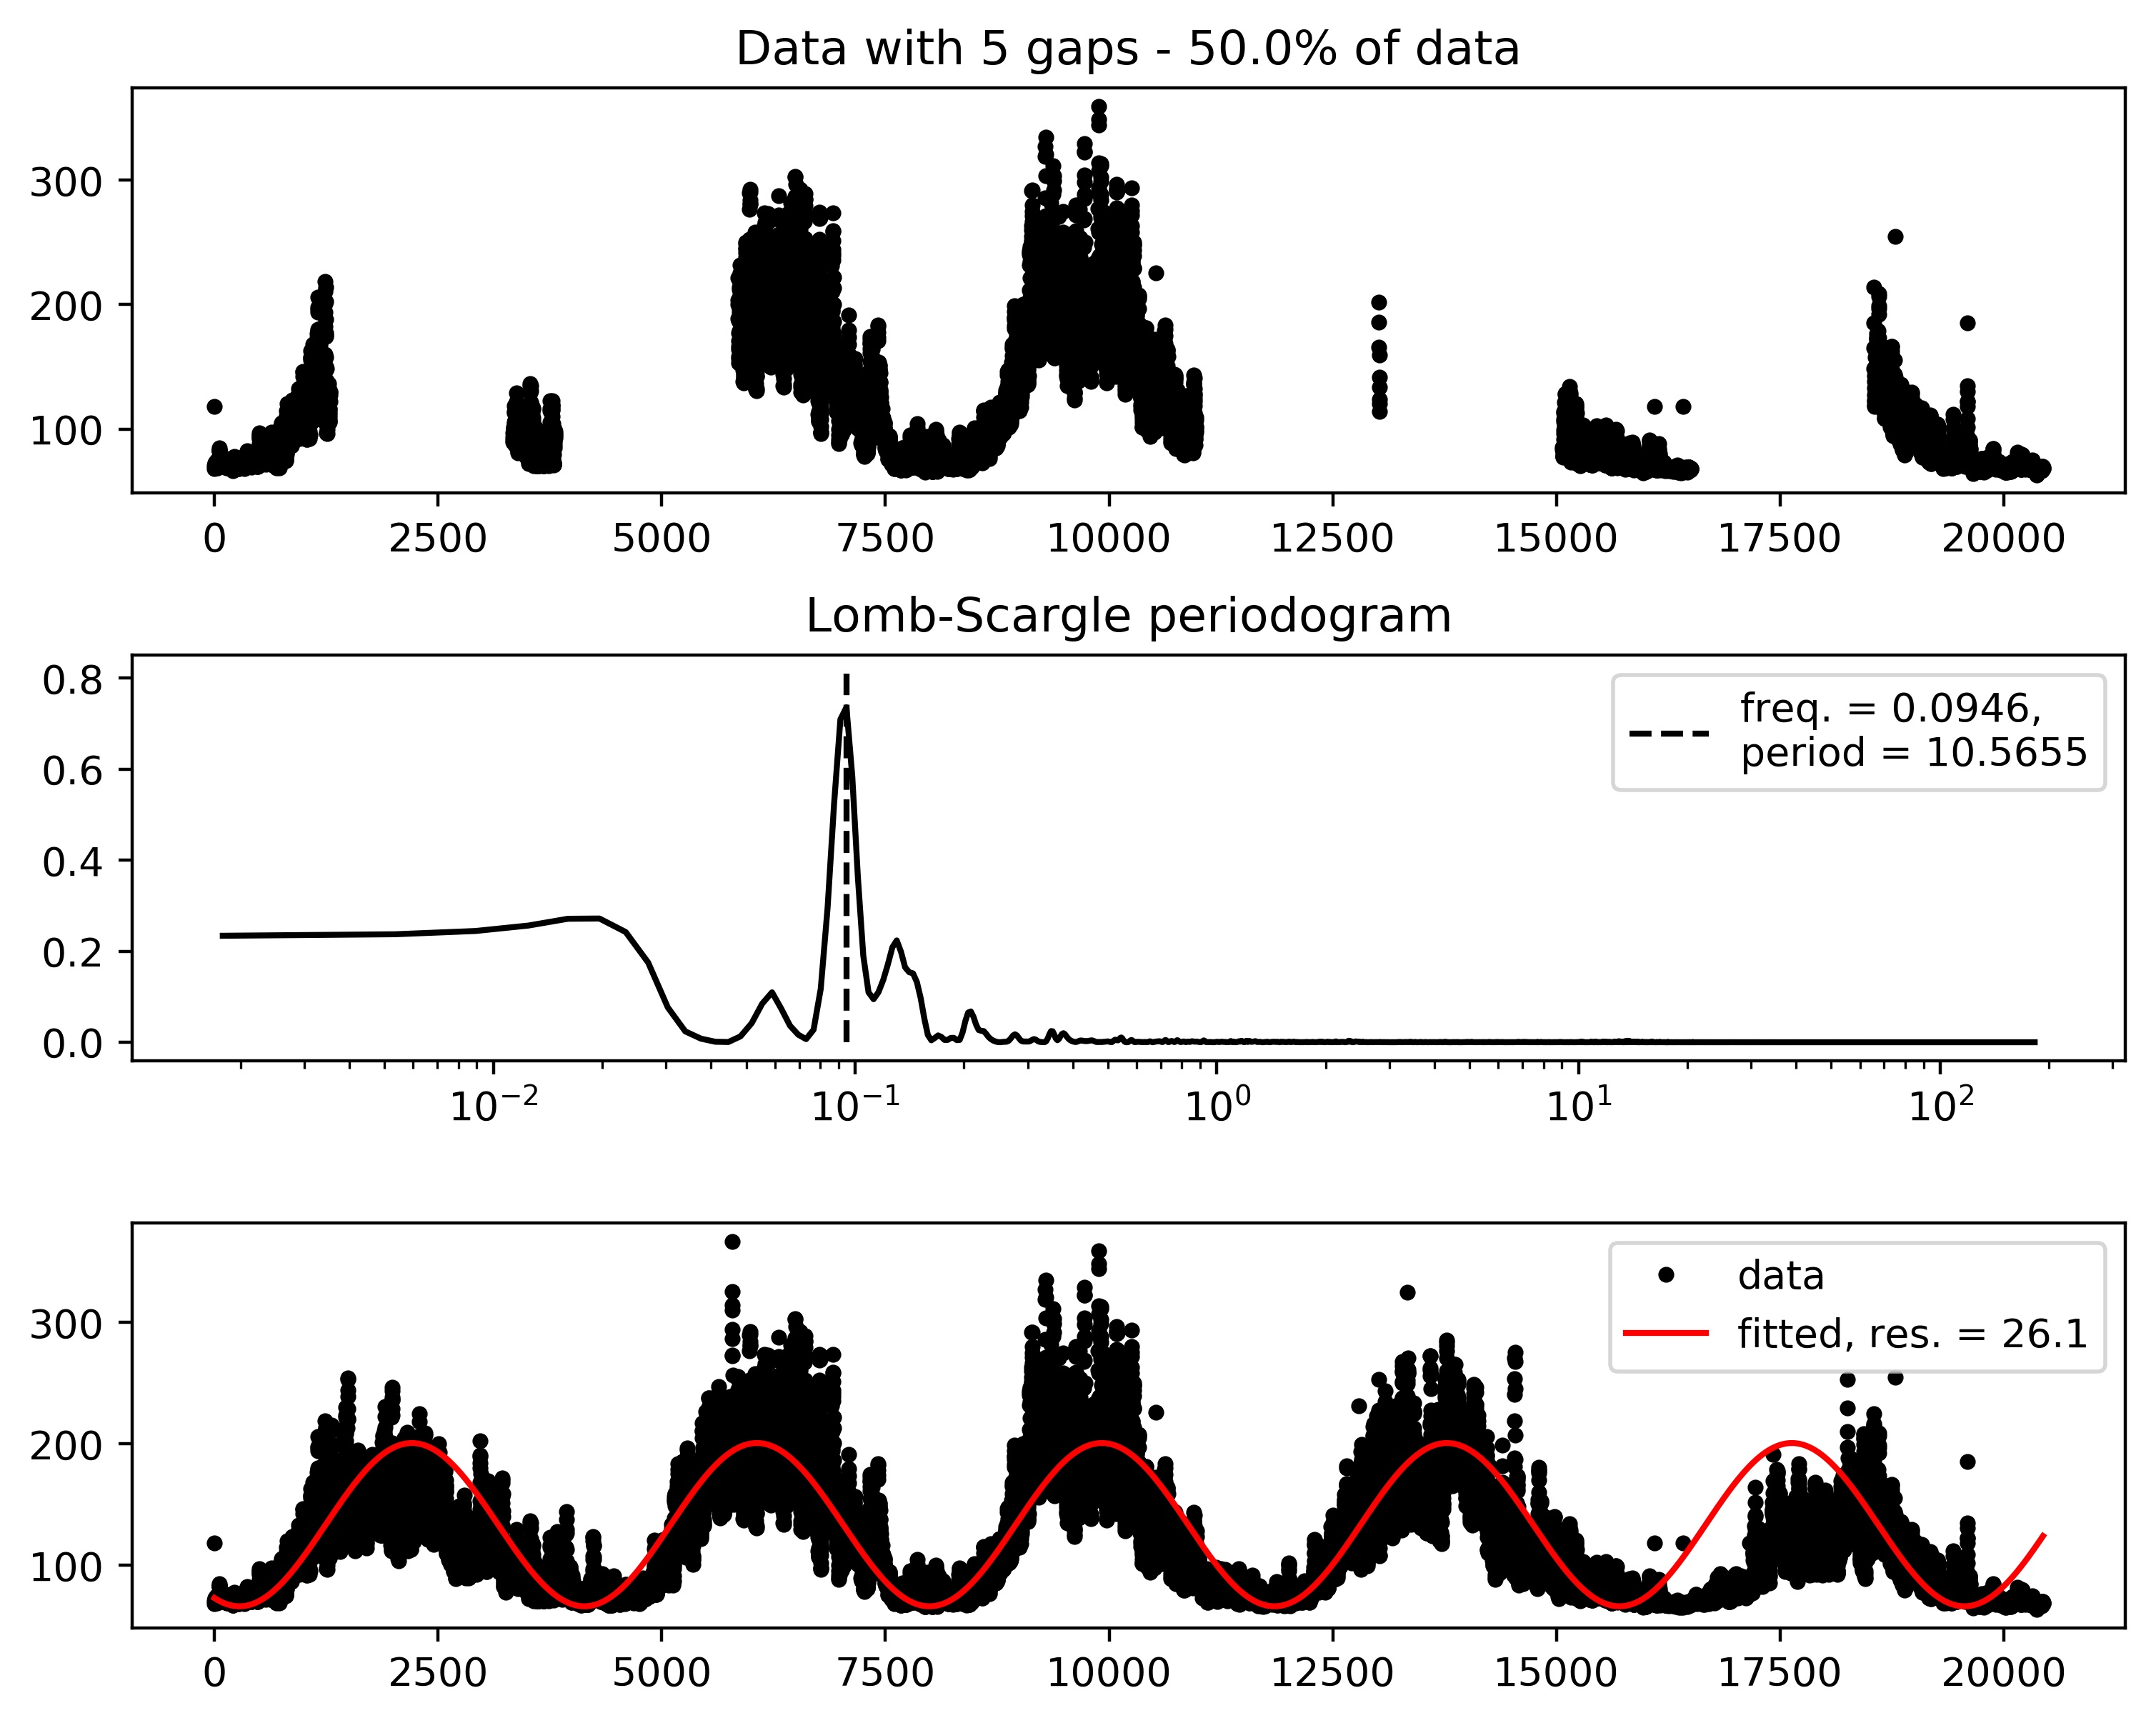
\includegraphics{../scripts/dataset1/periodograms_ny2.0_model2_Ng5.jpg}}
	\end{center}
	\vspace{-1mm}	
	\legenda{Resultado para 5 intervalos. Novamente a ferramenta utilizada corretamente identificou a periodicidade do sinal, e a função ajustada também corresponde bem à série original.}
	\label{fig:5gaps}
\end{figure}

\begin{figure}[ht!]
\vspace{-12mm}	
	\caption{Análise das médias diárias com 6 intervalos.}
	\vspace{1mm}	
	\begin{center}
		\resizebox{.8\textwidth}{!}{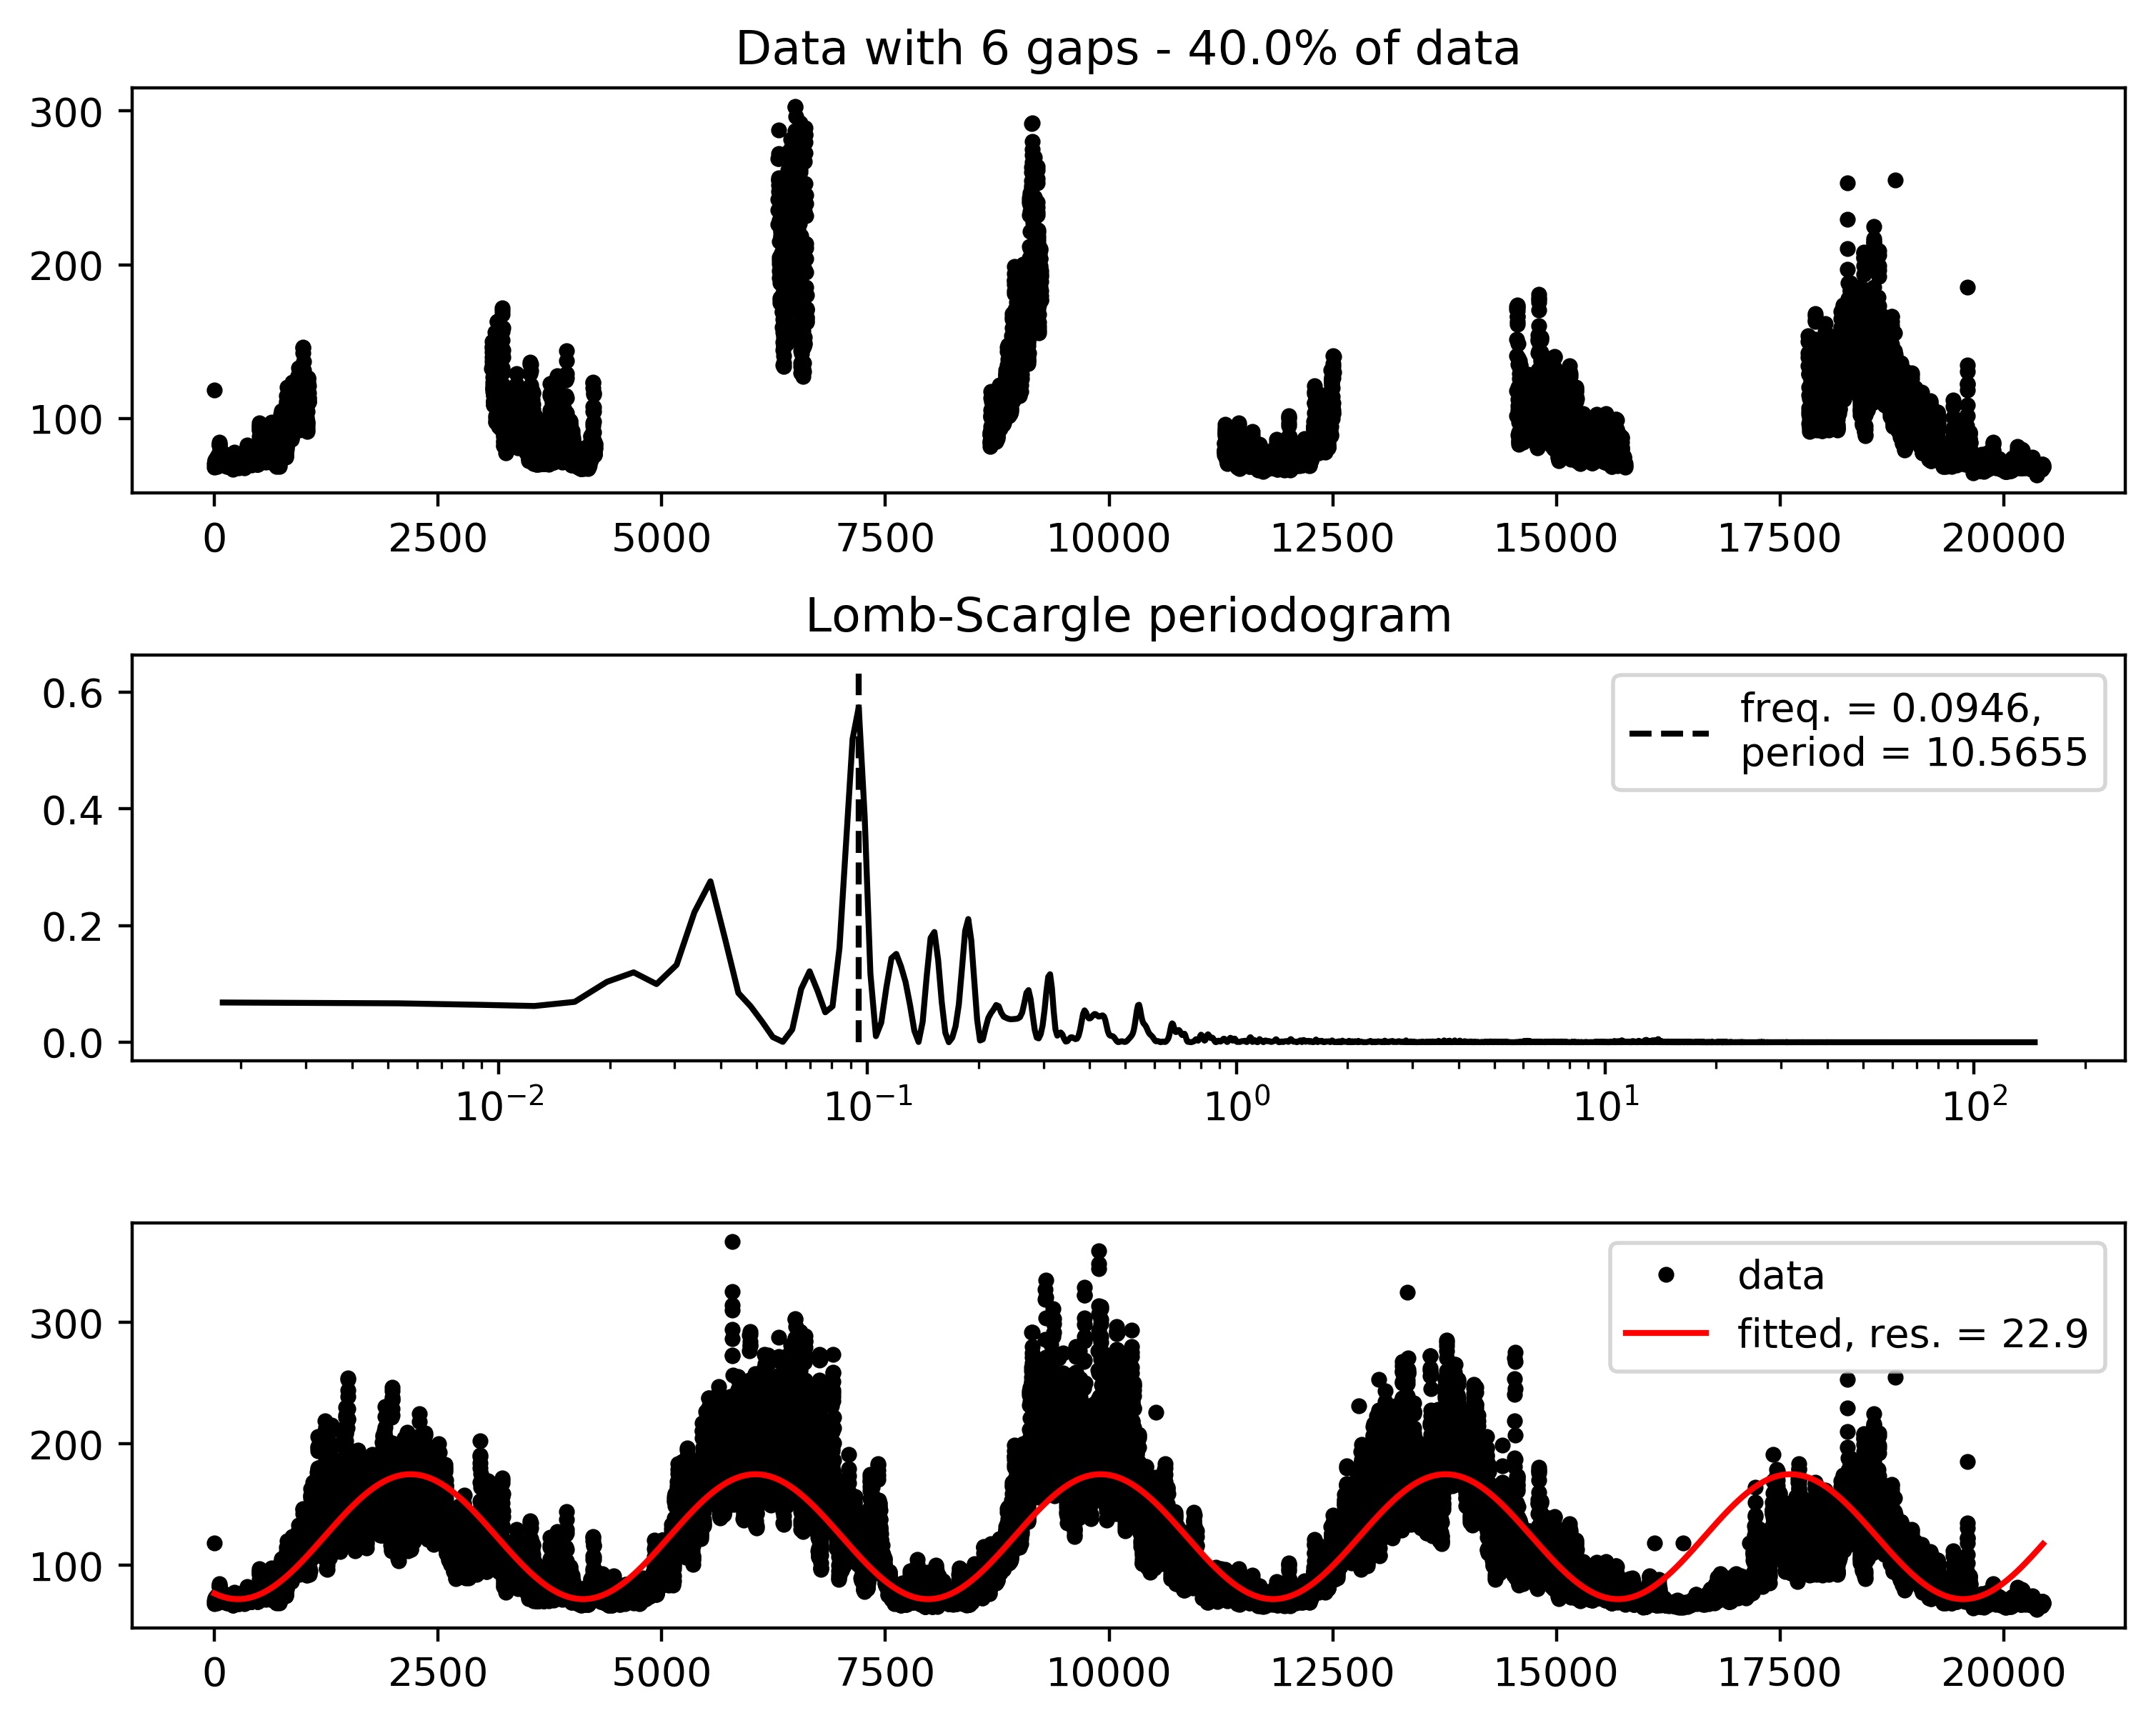
\includegraphics{../scripts/dataset1/periodograms_ny2.0_model2_Ng6.jpg}}
	\end{center}
	\vspace{-1mm}	
	\legenda{Resultado para 6 intervalos. Aqui mais frequências espúrias começam a surgir no periodograma, mas a principal assinatura ainda é bem identificada.}
	\label{fig:6gaps}
\end{figure}

\begin{figure}[ht!]
\vspace{-10mm}	
	\caption{Análise das médias diárias com 7 intervalos.}
	\vspace{1mm}	
	\begin{center}
		\resizebox{.8\textwidth}{!}{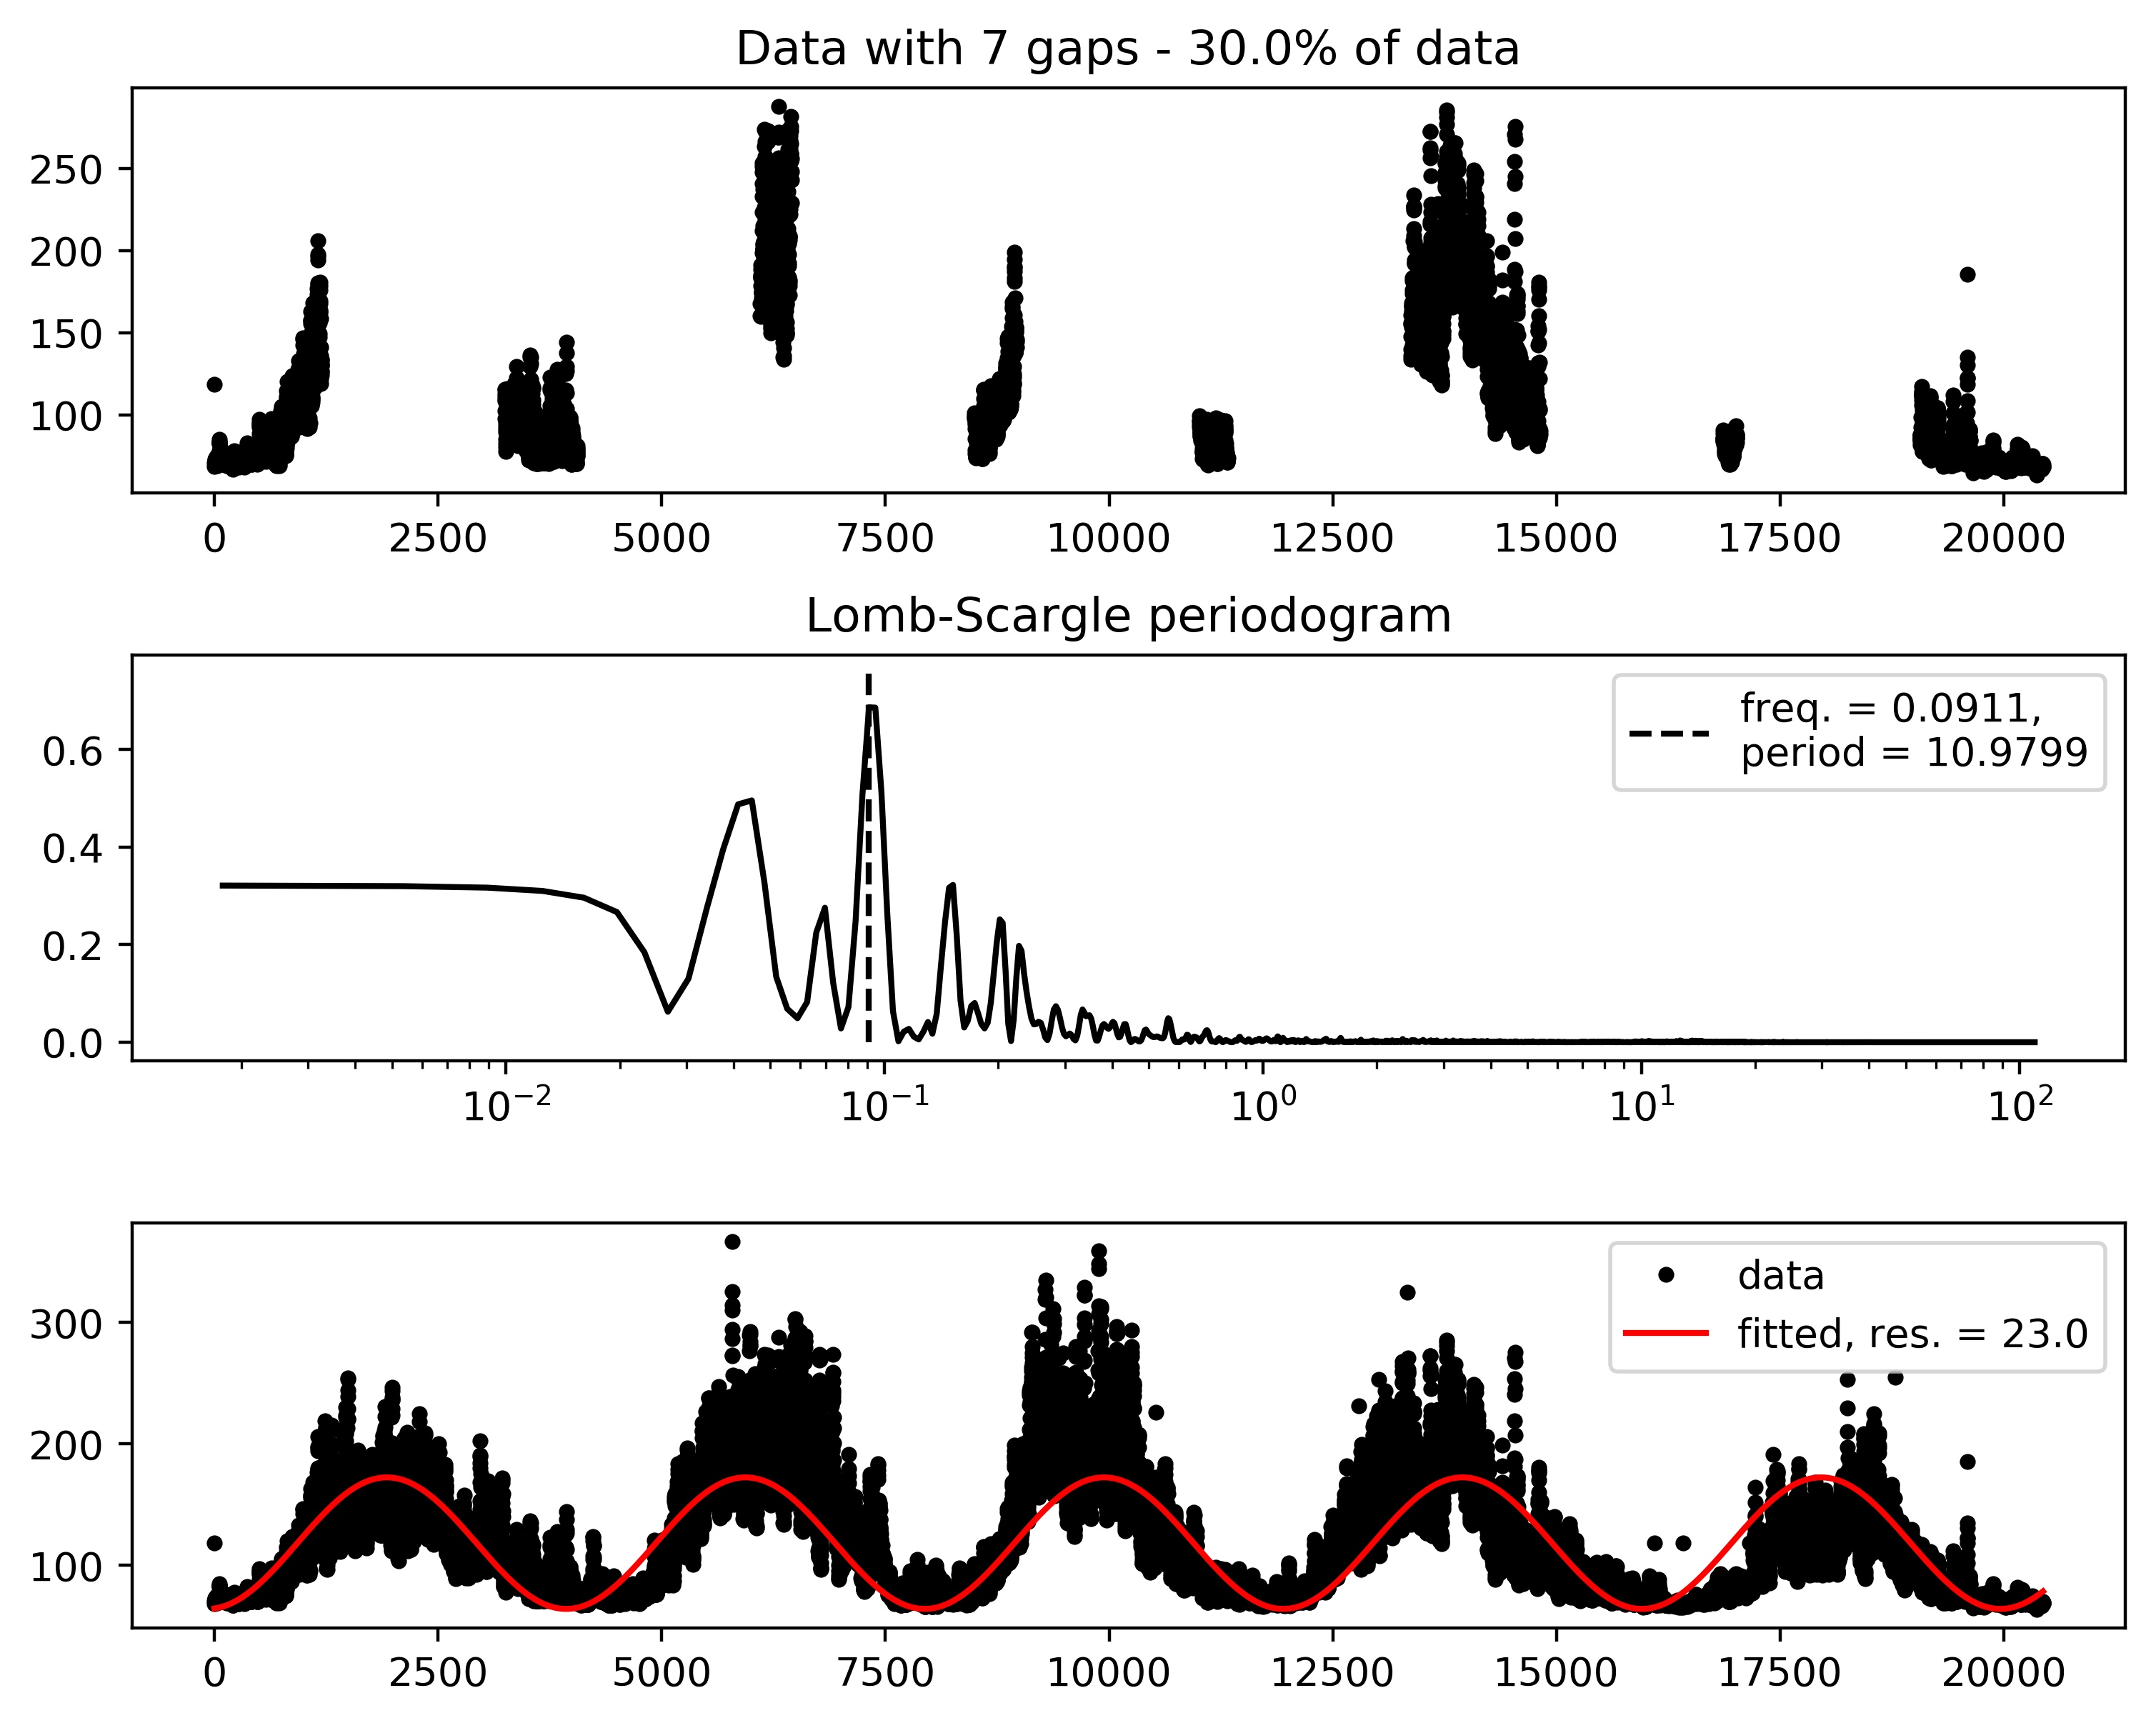
\includegraphics{../scripts/dataset1/periodograms_ny2.0_model2_Ng7.jpg}}
	\end{center}
	\vspace{-1mm}	
	\legenda{Resultado para 7 intervalos. Mesmo com somente 30\% dos dados, o resultado do periodograma de Lomb-Scargle se mostra consistente.}
	\label{fig:7gaps}
\end{figure}

\begin{figure}[ht!]
\vspace{-8mm}	
	\caption{Análise das médias diárias com 8 intervalos.}
	\vspace{1mm}	
	\begin{center}
		\resizebox{.8\textwidth}{!}{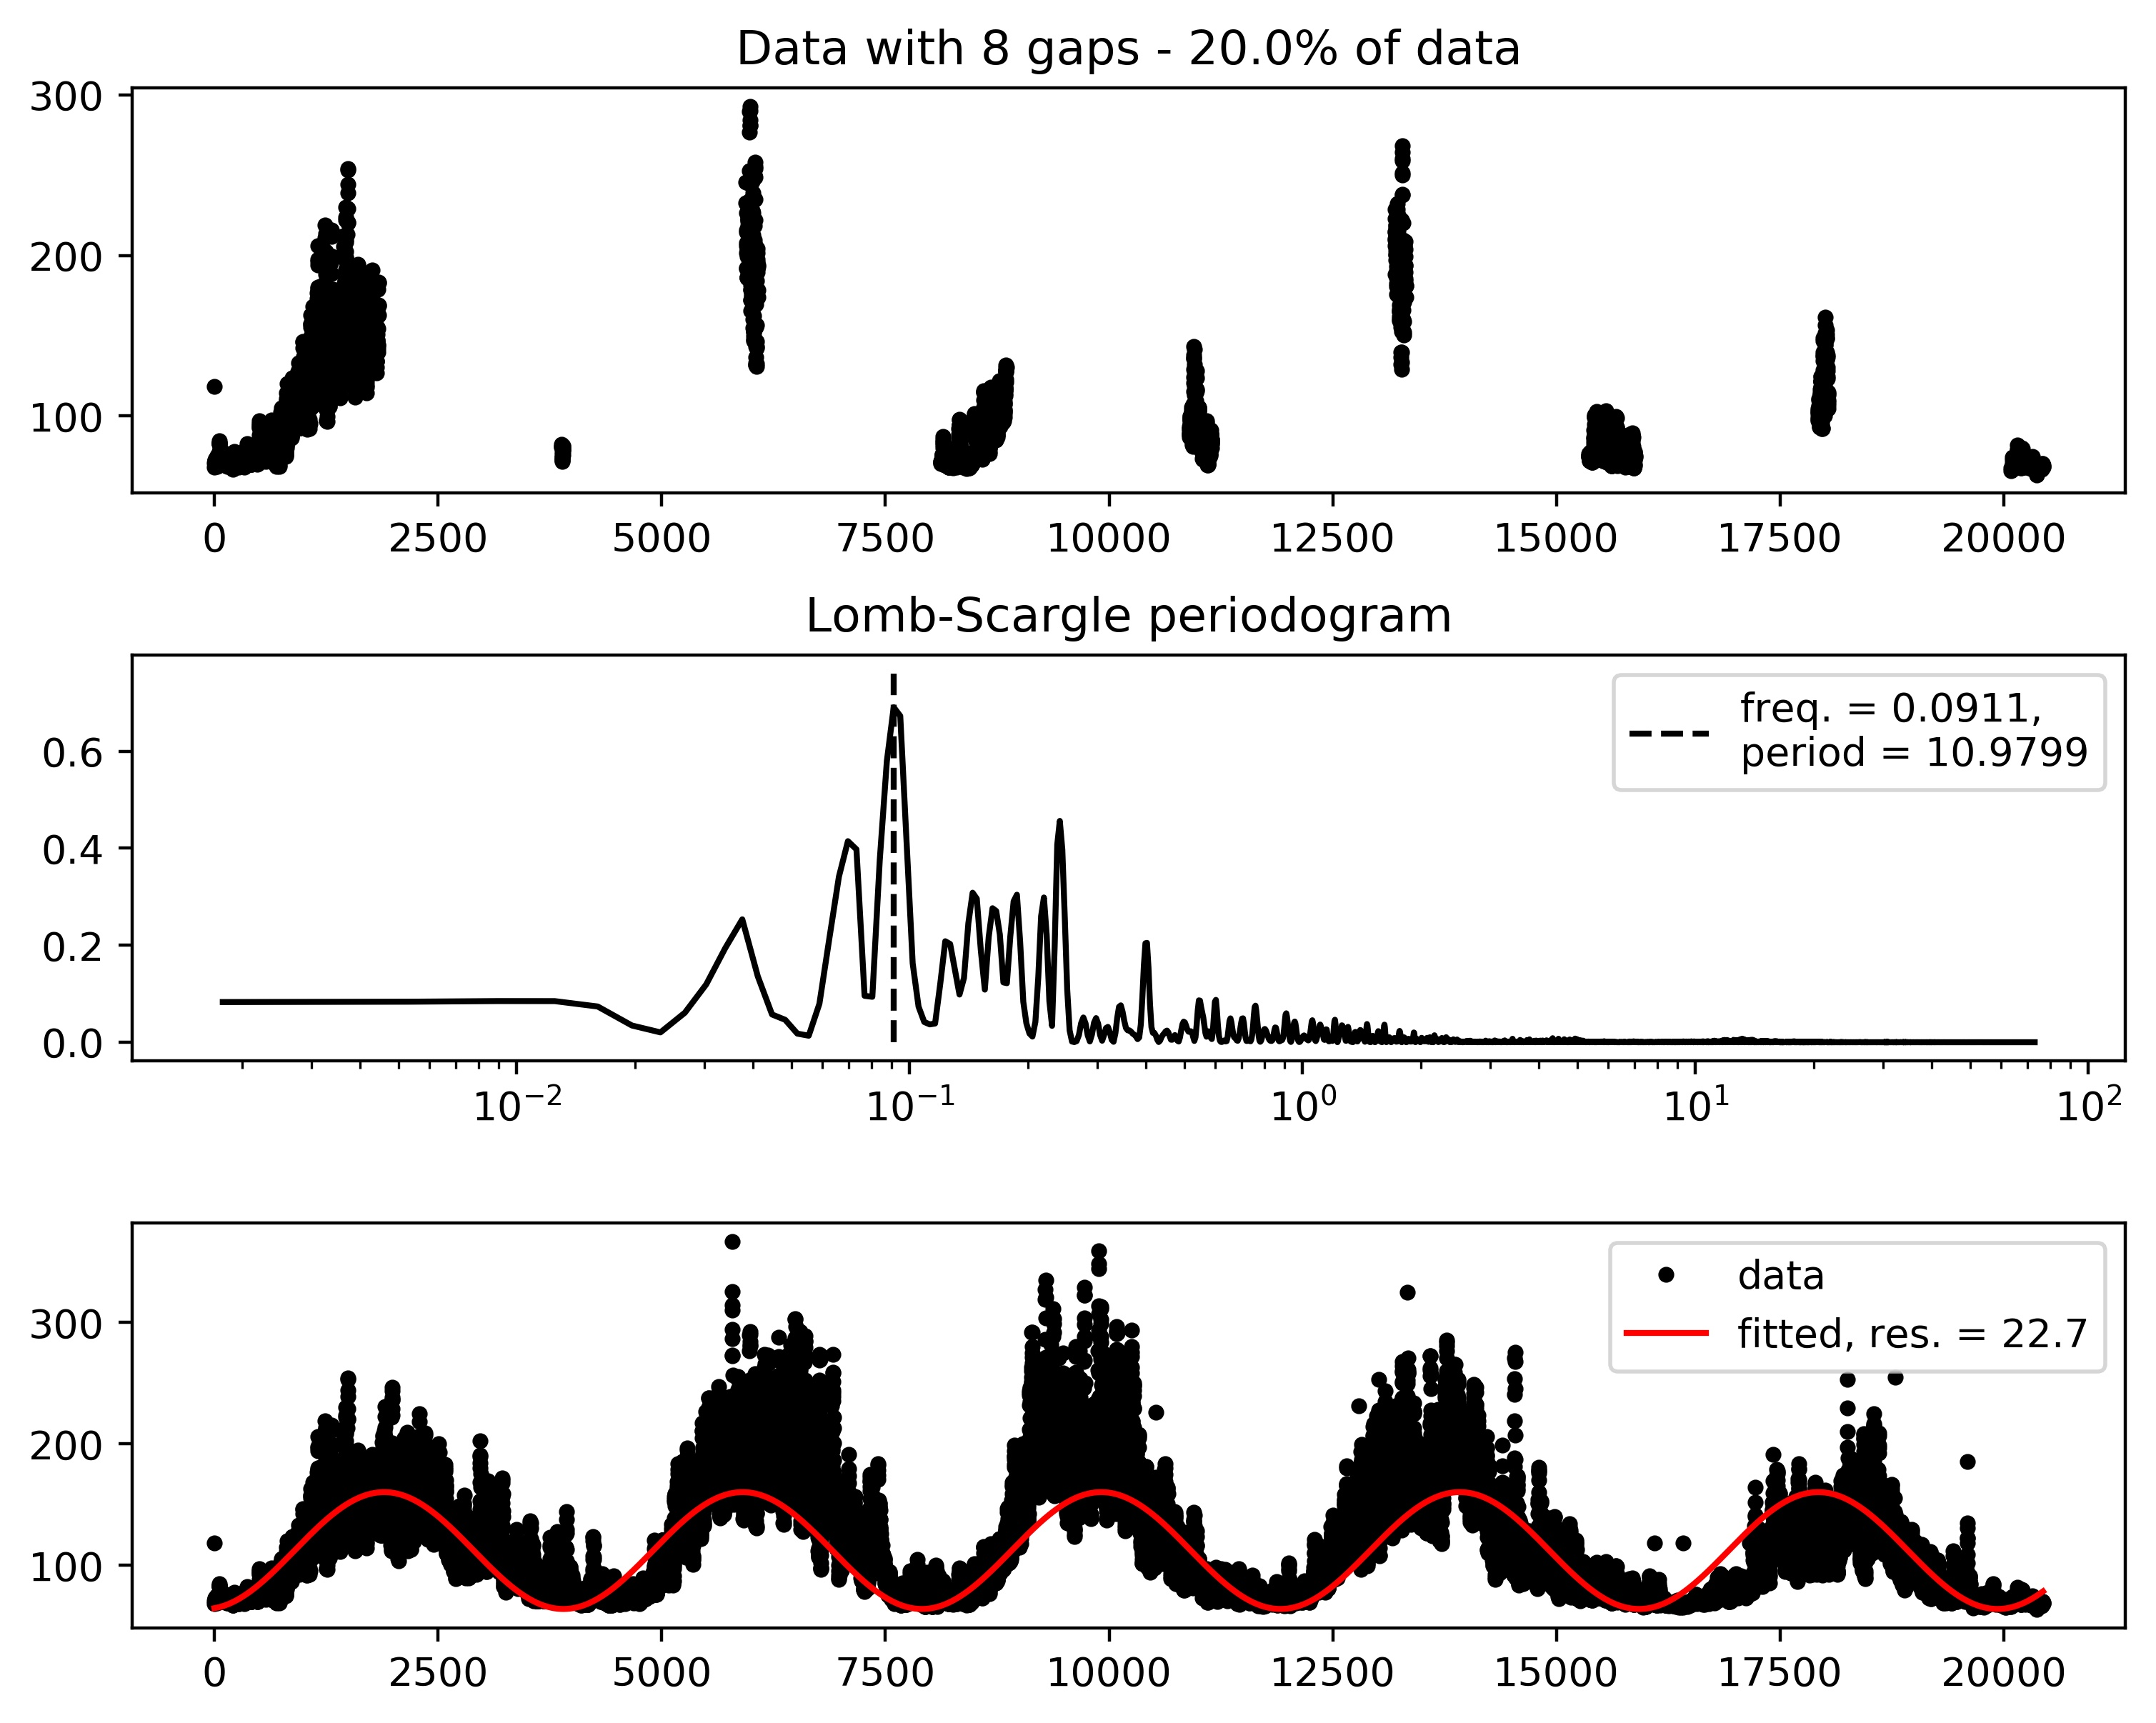
\includegraphics{../scripts/dataset1/periodograms_ny2.0_model2_Ng8.jpg}}
	\end{center}
	\vspace{-1mm}	
	\legenda{Resultado para 8 intervalos. A quantidade de picos espúrios próximo ao principal é maior que nos testes anteriores.}
	\label{fig:8gaps}
\end{figure}

\clearpage{}
\vspace*{-60px}	
Os resultados das Figuras \ref{fig:4gaps} a \ref{fig:8gaps} indicam que o periodograma de Lomb-Scargle é satisfatório em diversas situações de ausência de dados. A princípio, a Figura \ref{fig:4gaps} indica que a presença de poucos intervalos, tomando $\sim$40\% dos dados, não causa tantas anomalias ao periodograma. Os picos próximos ao principal (em 0.0946) são frequência que também se ajustaram bem aos dados. O resultado da melhor frequência foi aproximadamente o mesmo em todos os testes. Ao mesmo tempo, quanto maior o número de intervalos, maior foi a presença de picos espúrios. Neste sentido, as Figuras \ref{fig:7gaps} e \ref{fig:8gaps} ilustram uma característica (aleatória) do experimento: não só a quantidade de gaps, mas também a distribuição destes afetou a performance da ferramenta \texttt{LombScargle}, ainda que em menor grau. Ou seja, dependendo da posição dos intervalos durante um teste, os resultados com 6, 7 e 8 intervalos podiam ser igualmente bons, ruins, ou diferir substancialmente, mas sempre apresentando mais picos espúrios que os resultados com 4 ou 5 intervalos.

	
\section{Cenário 2 - exclusão aleatória de dados}
		
O cenário testado a seguir se baseia na exclusão aleatória das amostras até que se chegue a um limite estabelecido de porcentagem do total inicial. Esse limite foi variado cinco vezes, de modo que restasse entre 1\% e 0.04\% dos dados de média diária do fluxo 10.7. %Demais resultados estão presentes em LINK DO REPOSITORIO.

\begin{figure}[ht!]
\vspace{-10mm}	
	\caption{Análise com exclusão aleatória até 1\% dos dados.}
	\vspace{0mm}	
	\begin{center}
		\resizebox{.8\textwidth}{!}{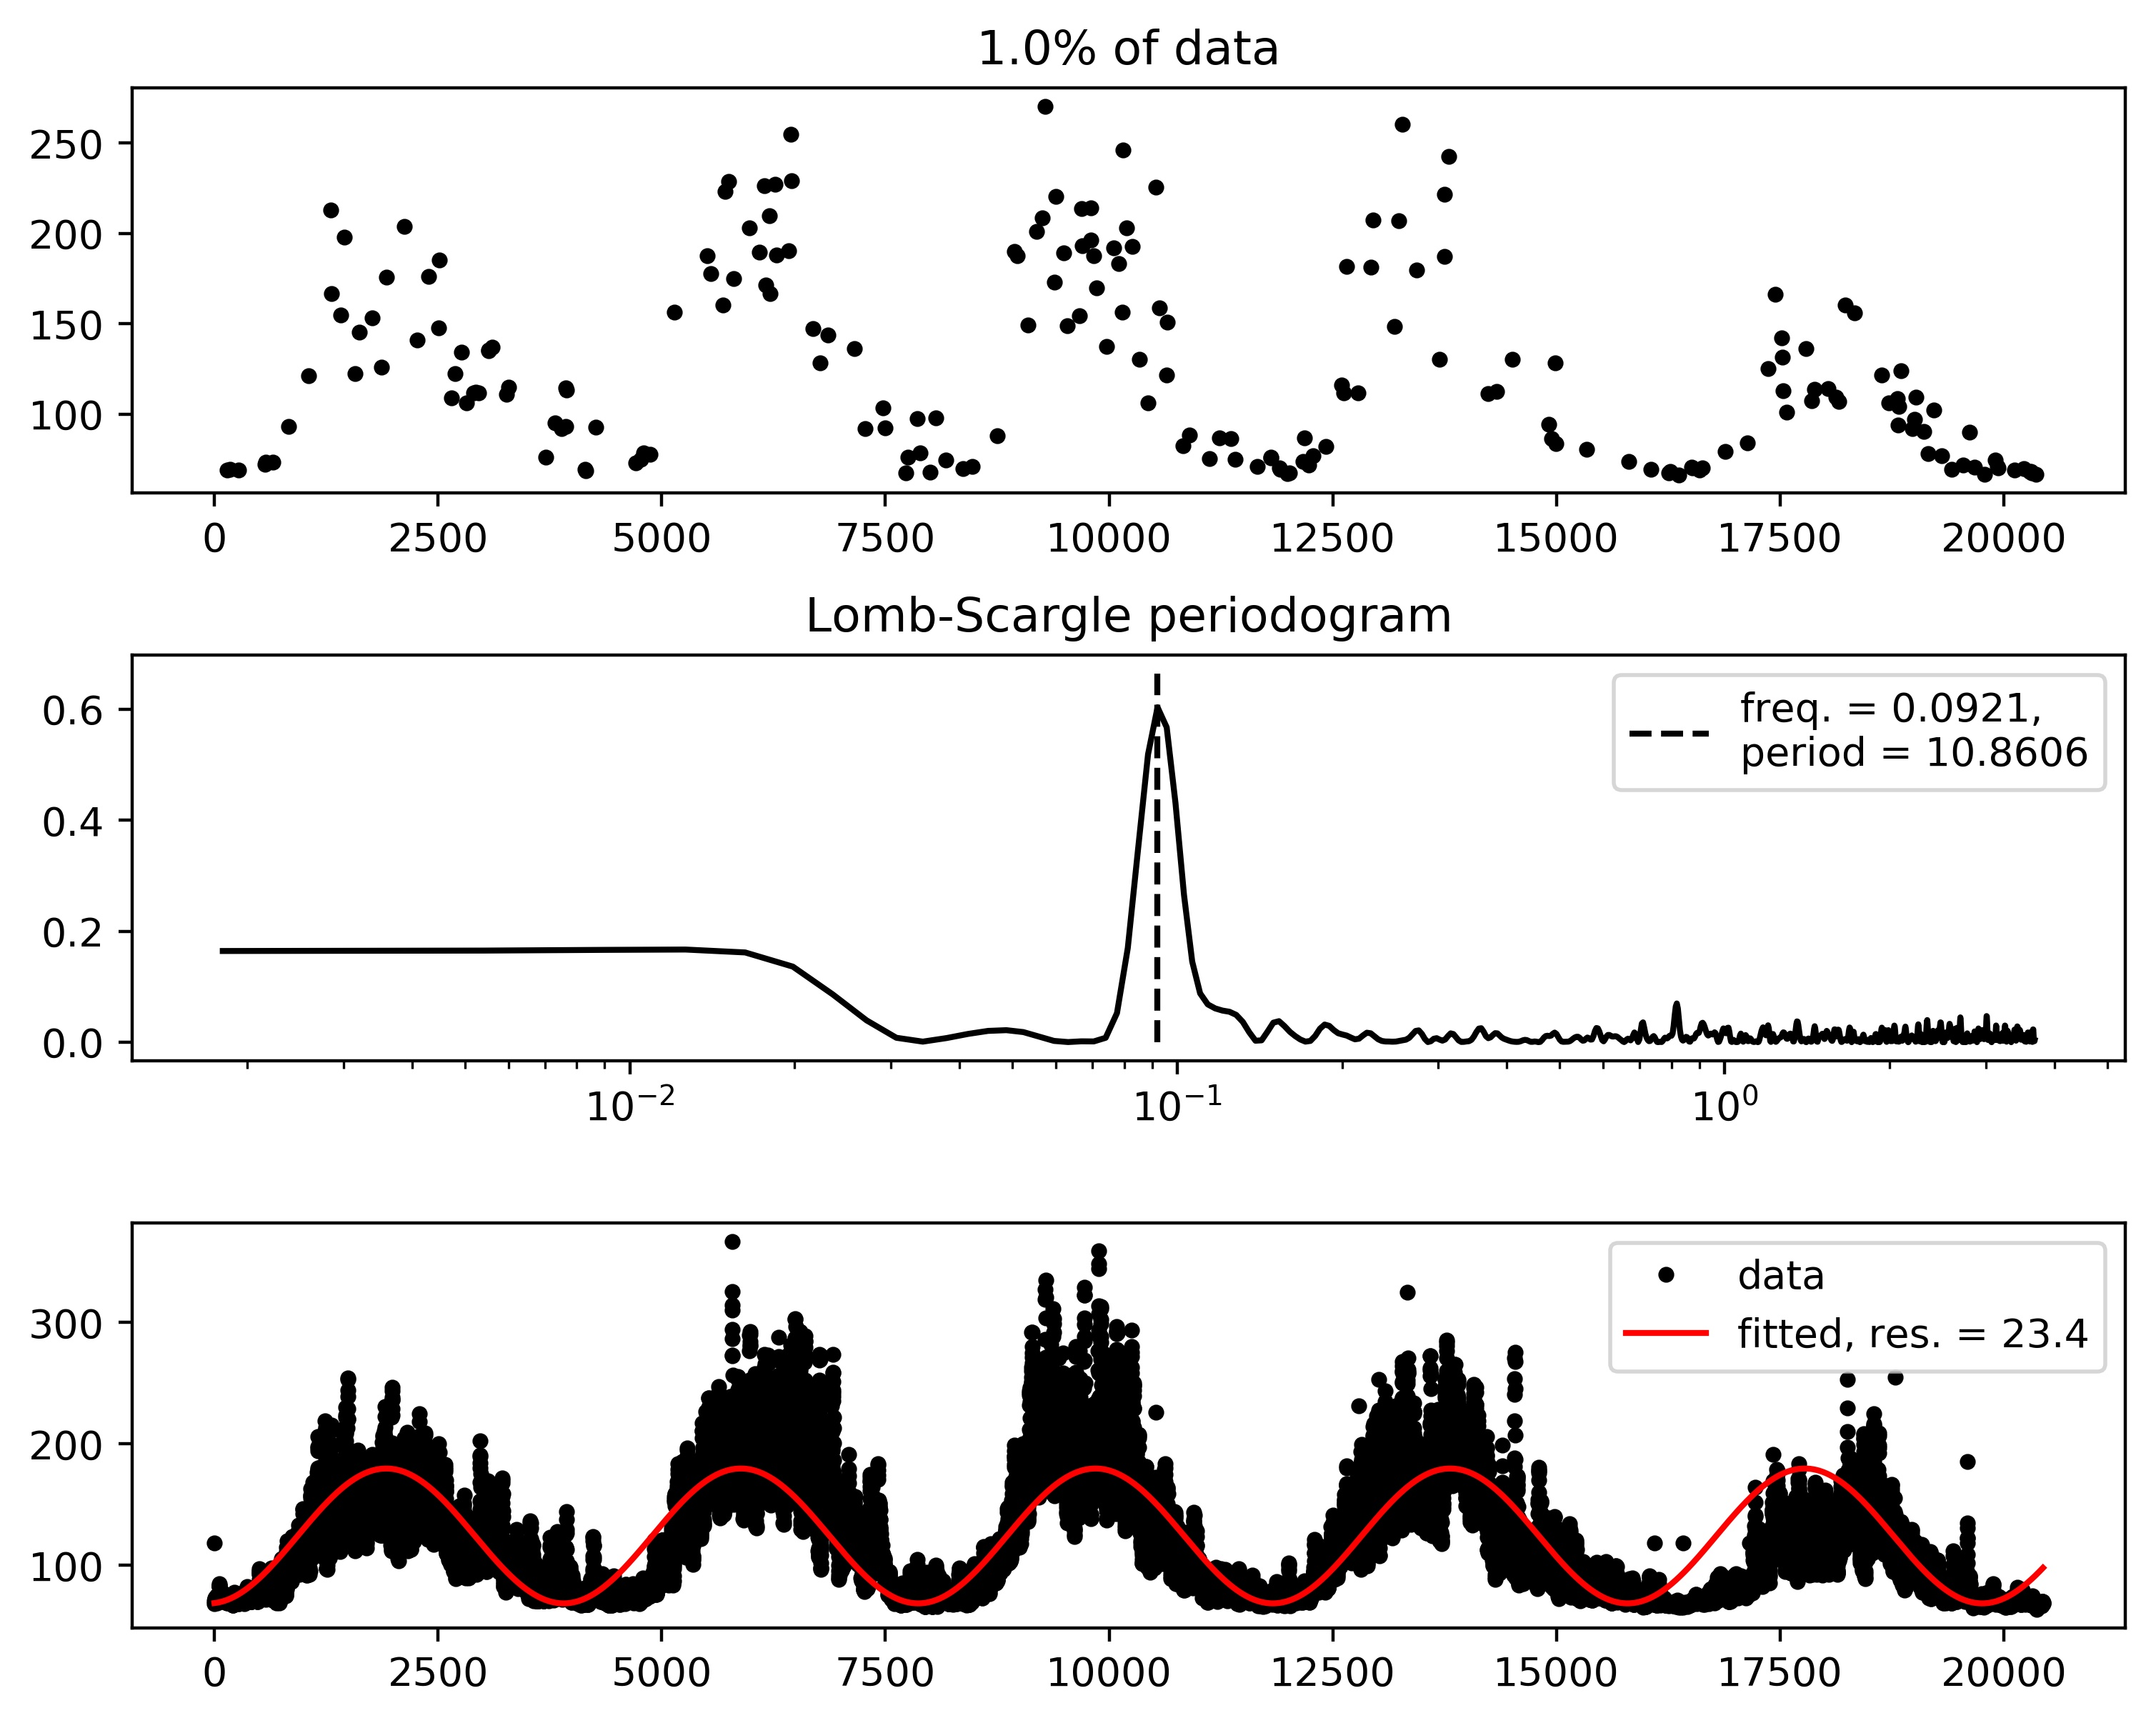
\includegraphics{../scripts/dataset1/periodograms_ny2.0_model1_pg0.99.jpg}}
	\end{center}
	\vspace{-1mm}	
	\legenda{A série original continha $\sim$20000 amostras, de modo que 1\% destes dados, ainda que aleatoriamente distribuídos, é capaz não só de indicar o formato original da série (graças aos nossos olhos e nossa capacidade de identificar padrões) mas também de ser analisada com excelência via periodograma de Lomb-Scargle (graças à classe \texttt{LoombScargle}).}
	\label{fig:percent1}
	\vspace{-8mm}	
\end{figure}

\begin{figure}[ht!]
\vspace{-14mm}	
	\caption{Análise com exclusão aleatória até 0.5\% dos dados.}
	\vspace{1mm}	
	\begin{center}
		\resizebox{.8\textwidth}{!}{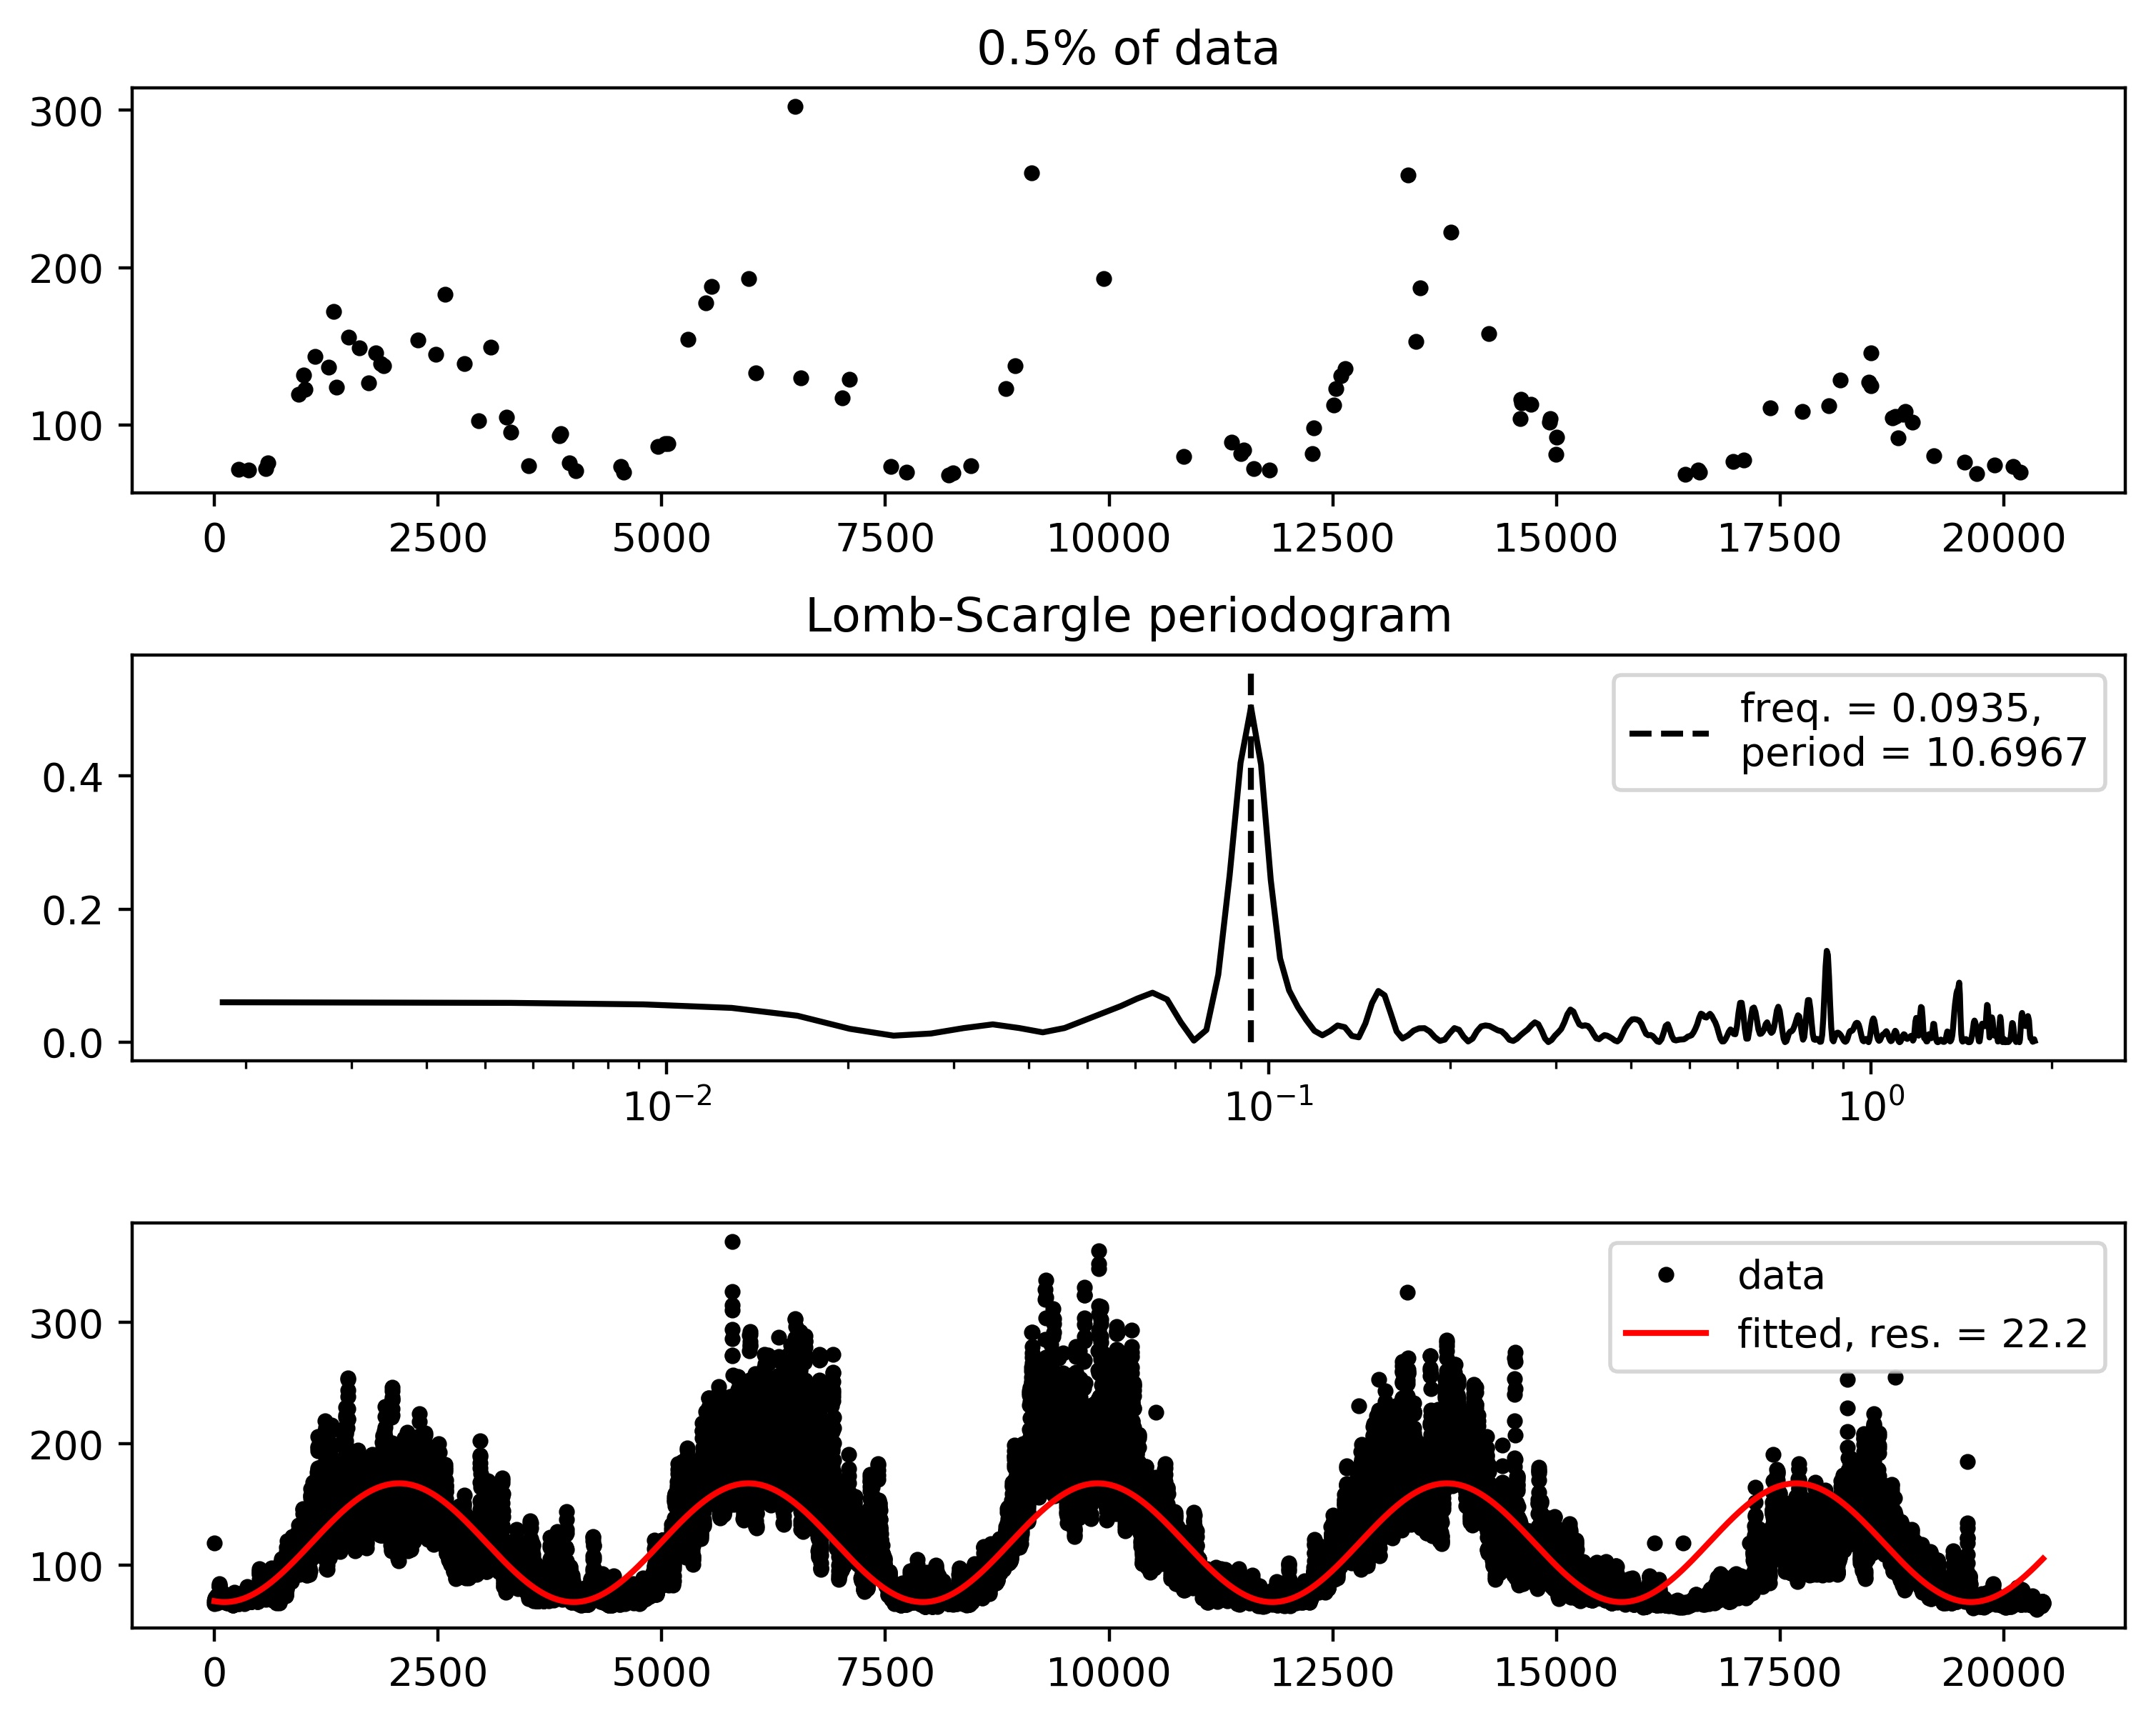
\includegraphics{../scripts/dataset1/periodograms_ny2.0_model1_pg0.995.jpg}}
	\end{center}
	\vspace{-1mm}	
	\legenda{Com 0.5\% dos dados a série se apresenta mais descaracterizada, mas com pontos suficientes para se assemelhar à a série original. O periodograma de Lomb-Scargle foi aplicado com sucesso.}
	\label{fig:percent0.5}
	\vspace{-3mm}
\end{figure}

\begin{figure}[ht!]
\vspace{-12mm}	
	\caption{Análise com exclusão aleatória até 0.1\% dos dados.}
	\vspace{1mm}	
	\begin{center}
		\resizebox{.8\textwidth}{!}{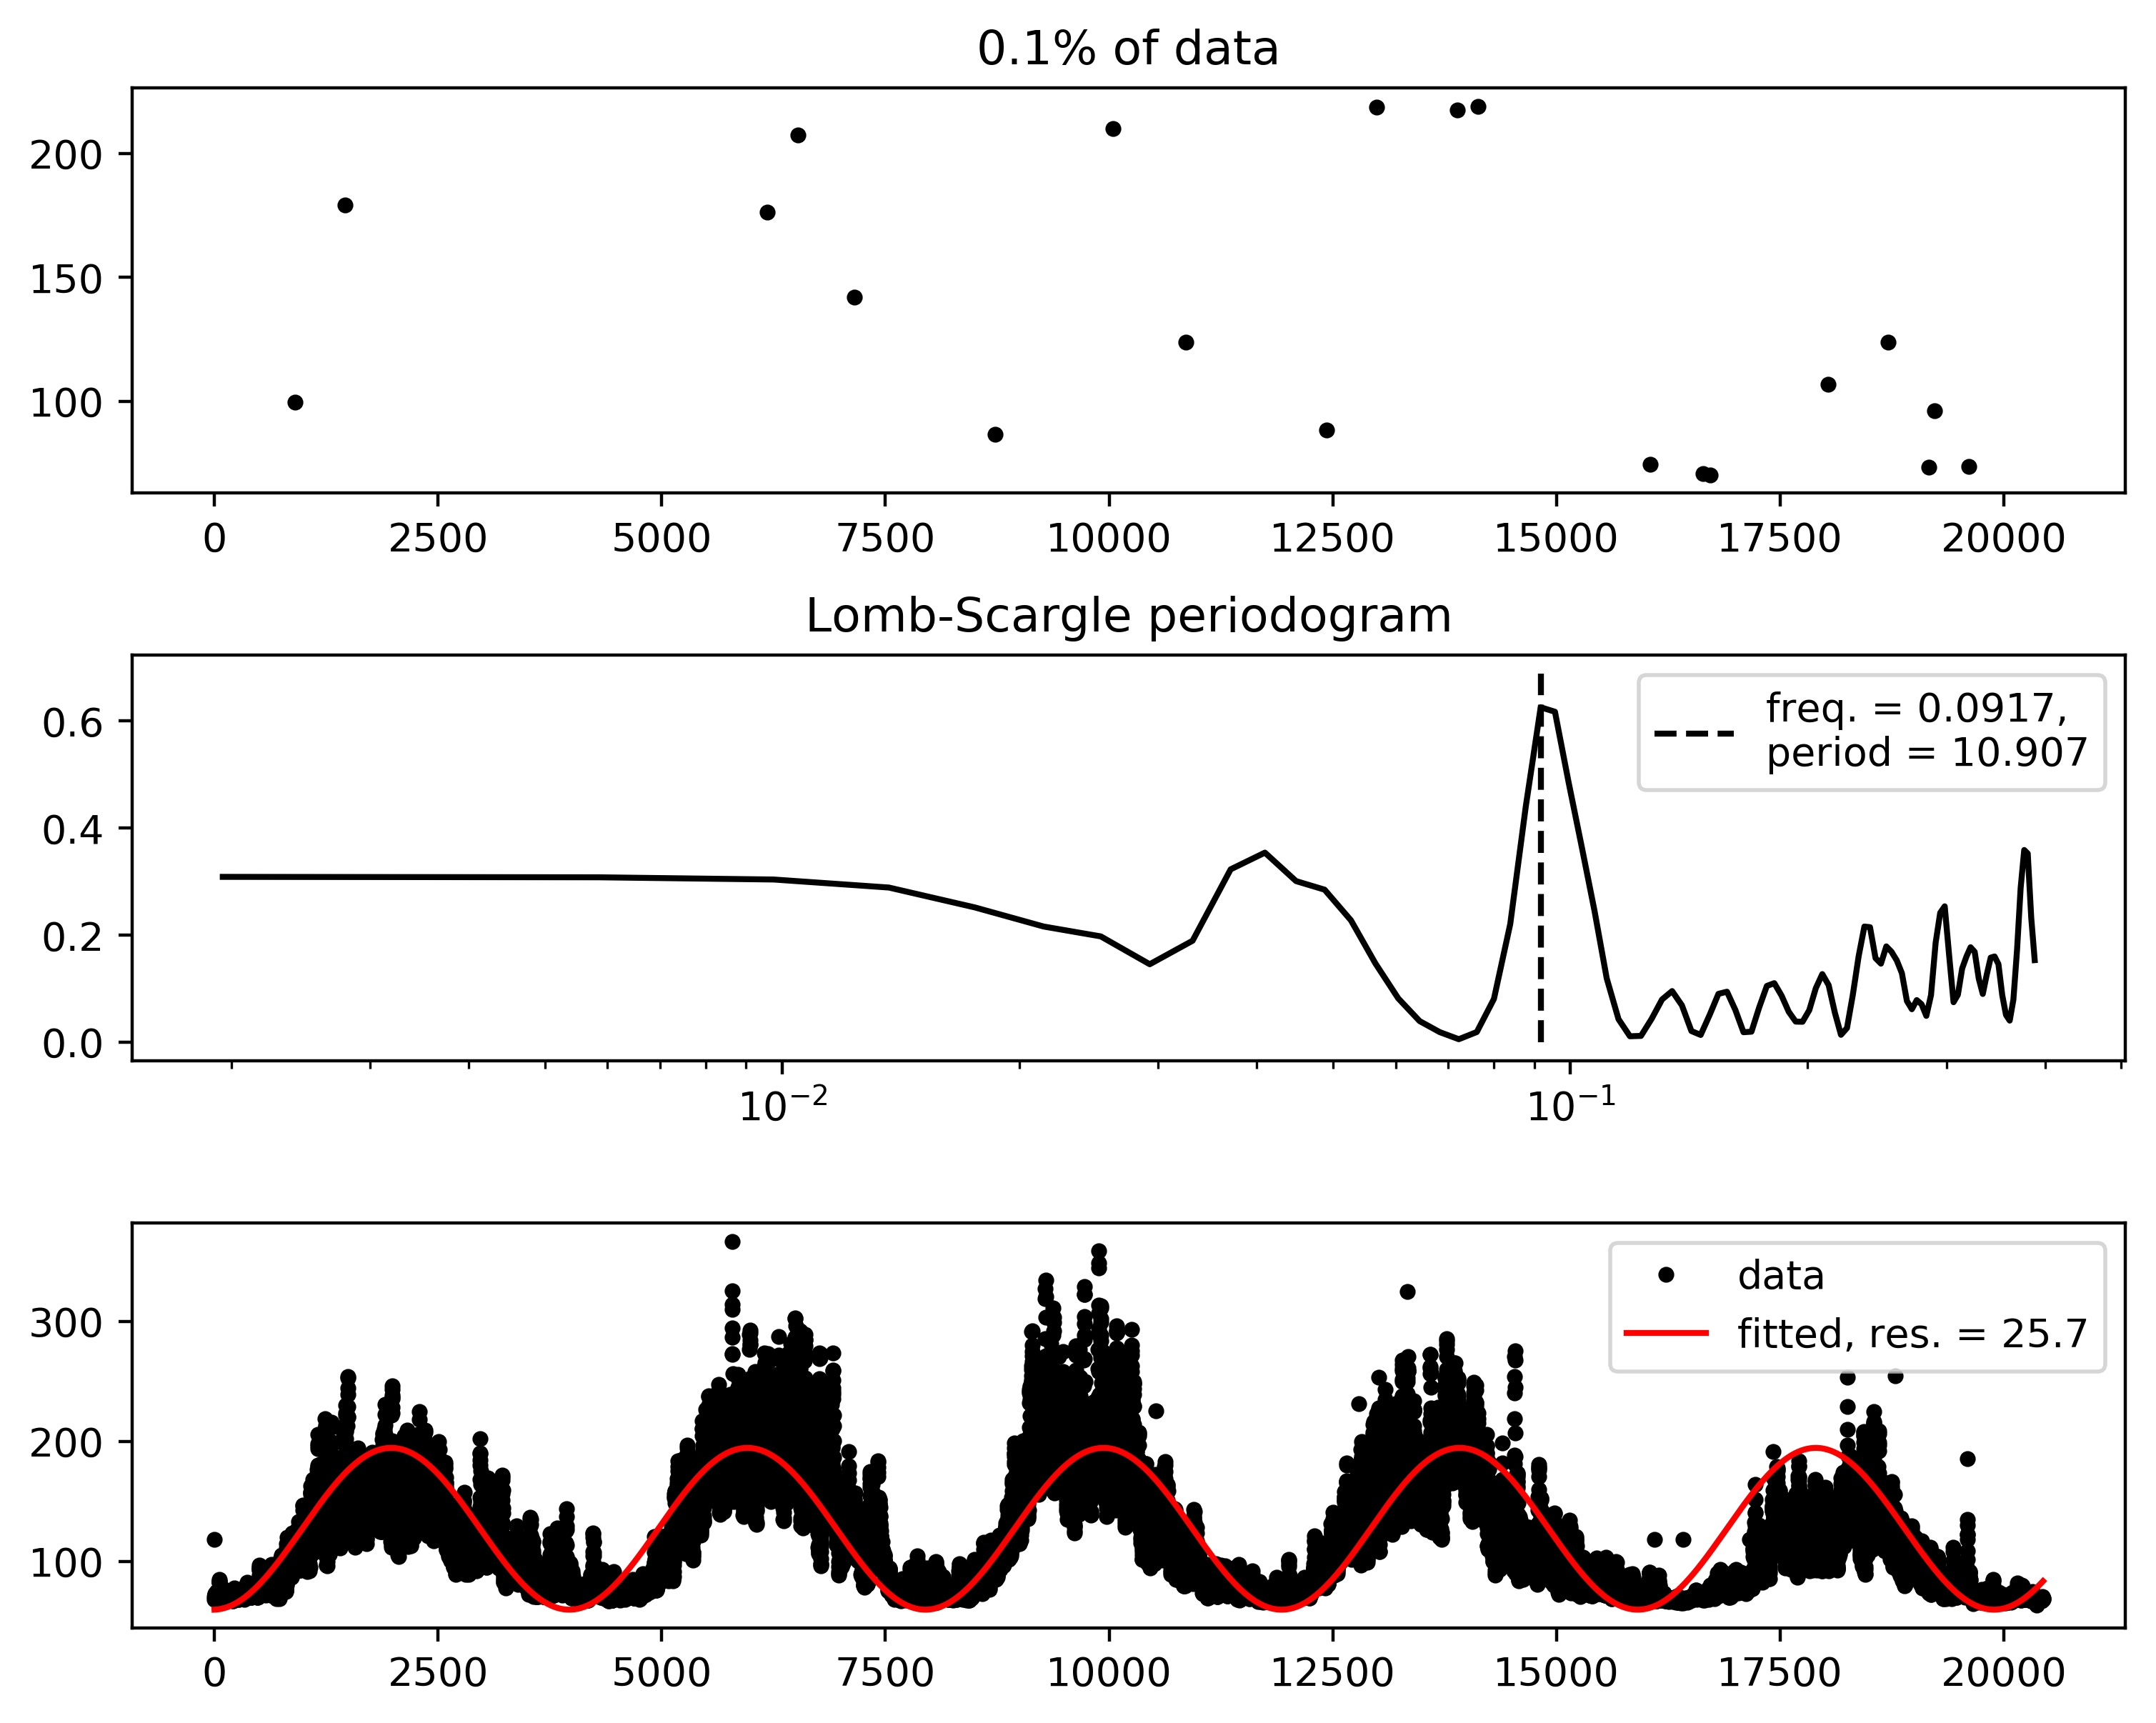
\includegraphics{../scripts/dataset1/periodograms_ny2.0_model1_pg0.999.jpg}}
	\end{center}
	\vspace{-1mm}	
	\legenda{Com somente 0.1\% dos dados, o perfil da série não é mais aparente e no periodograma surgem frequências espúrias. O período de $\sim$11 anos continua sendo corretamente determinado pela ferramenta.}
	\label{fig:percent0.1}
	\vspace{-5mm}	
\end{figure}

\begin{figure}[ht!]
\vspace{-10mm}	
	\caption{Análise com exclusão aleatória até 0.05\% dos dados.}
	\vspace{1mm}	
	\begin{center}
		\resizebox{.8\textwidth}{!}{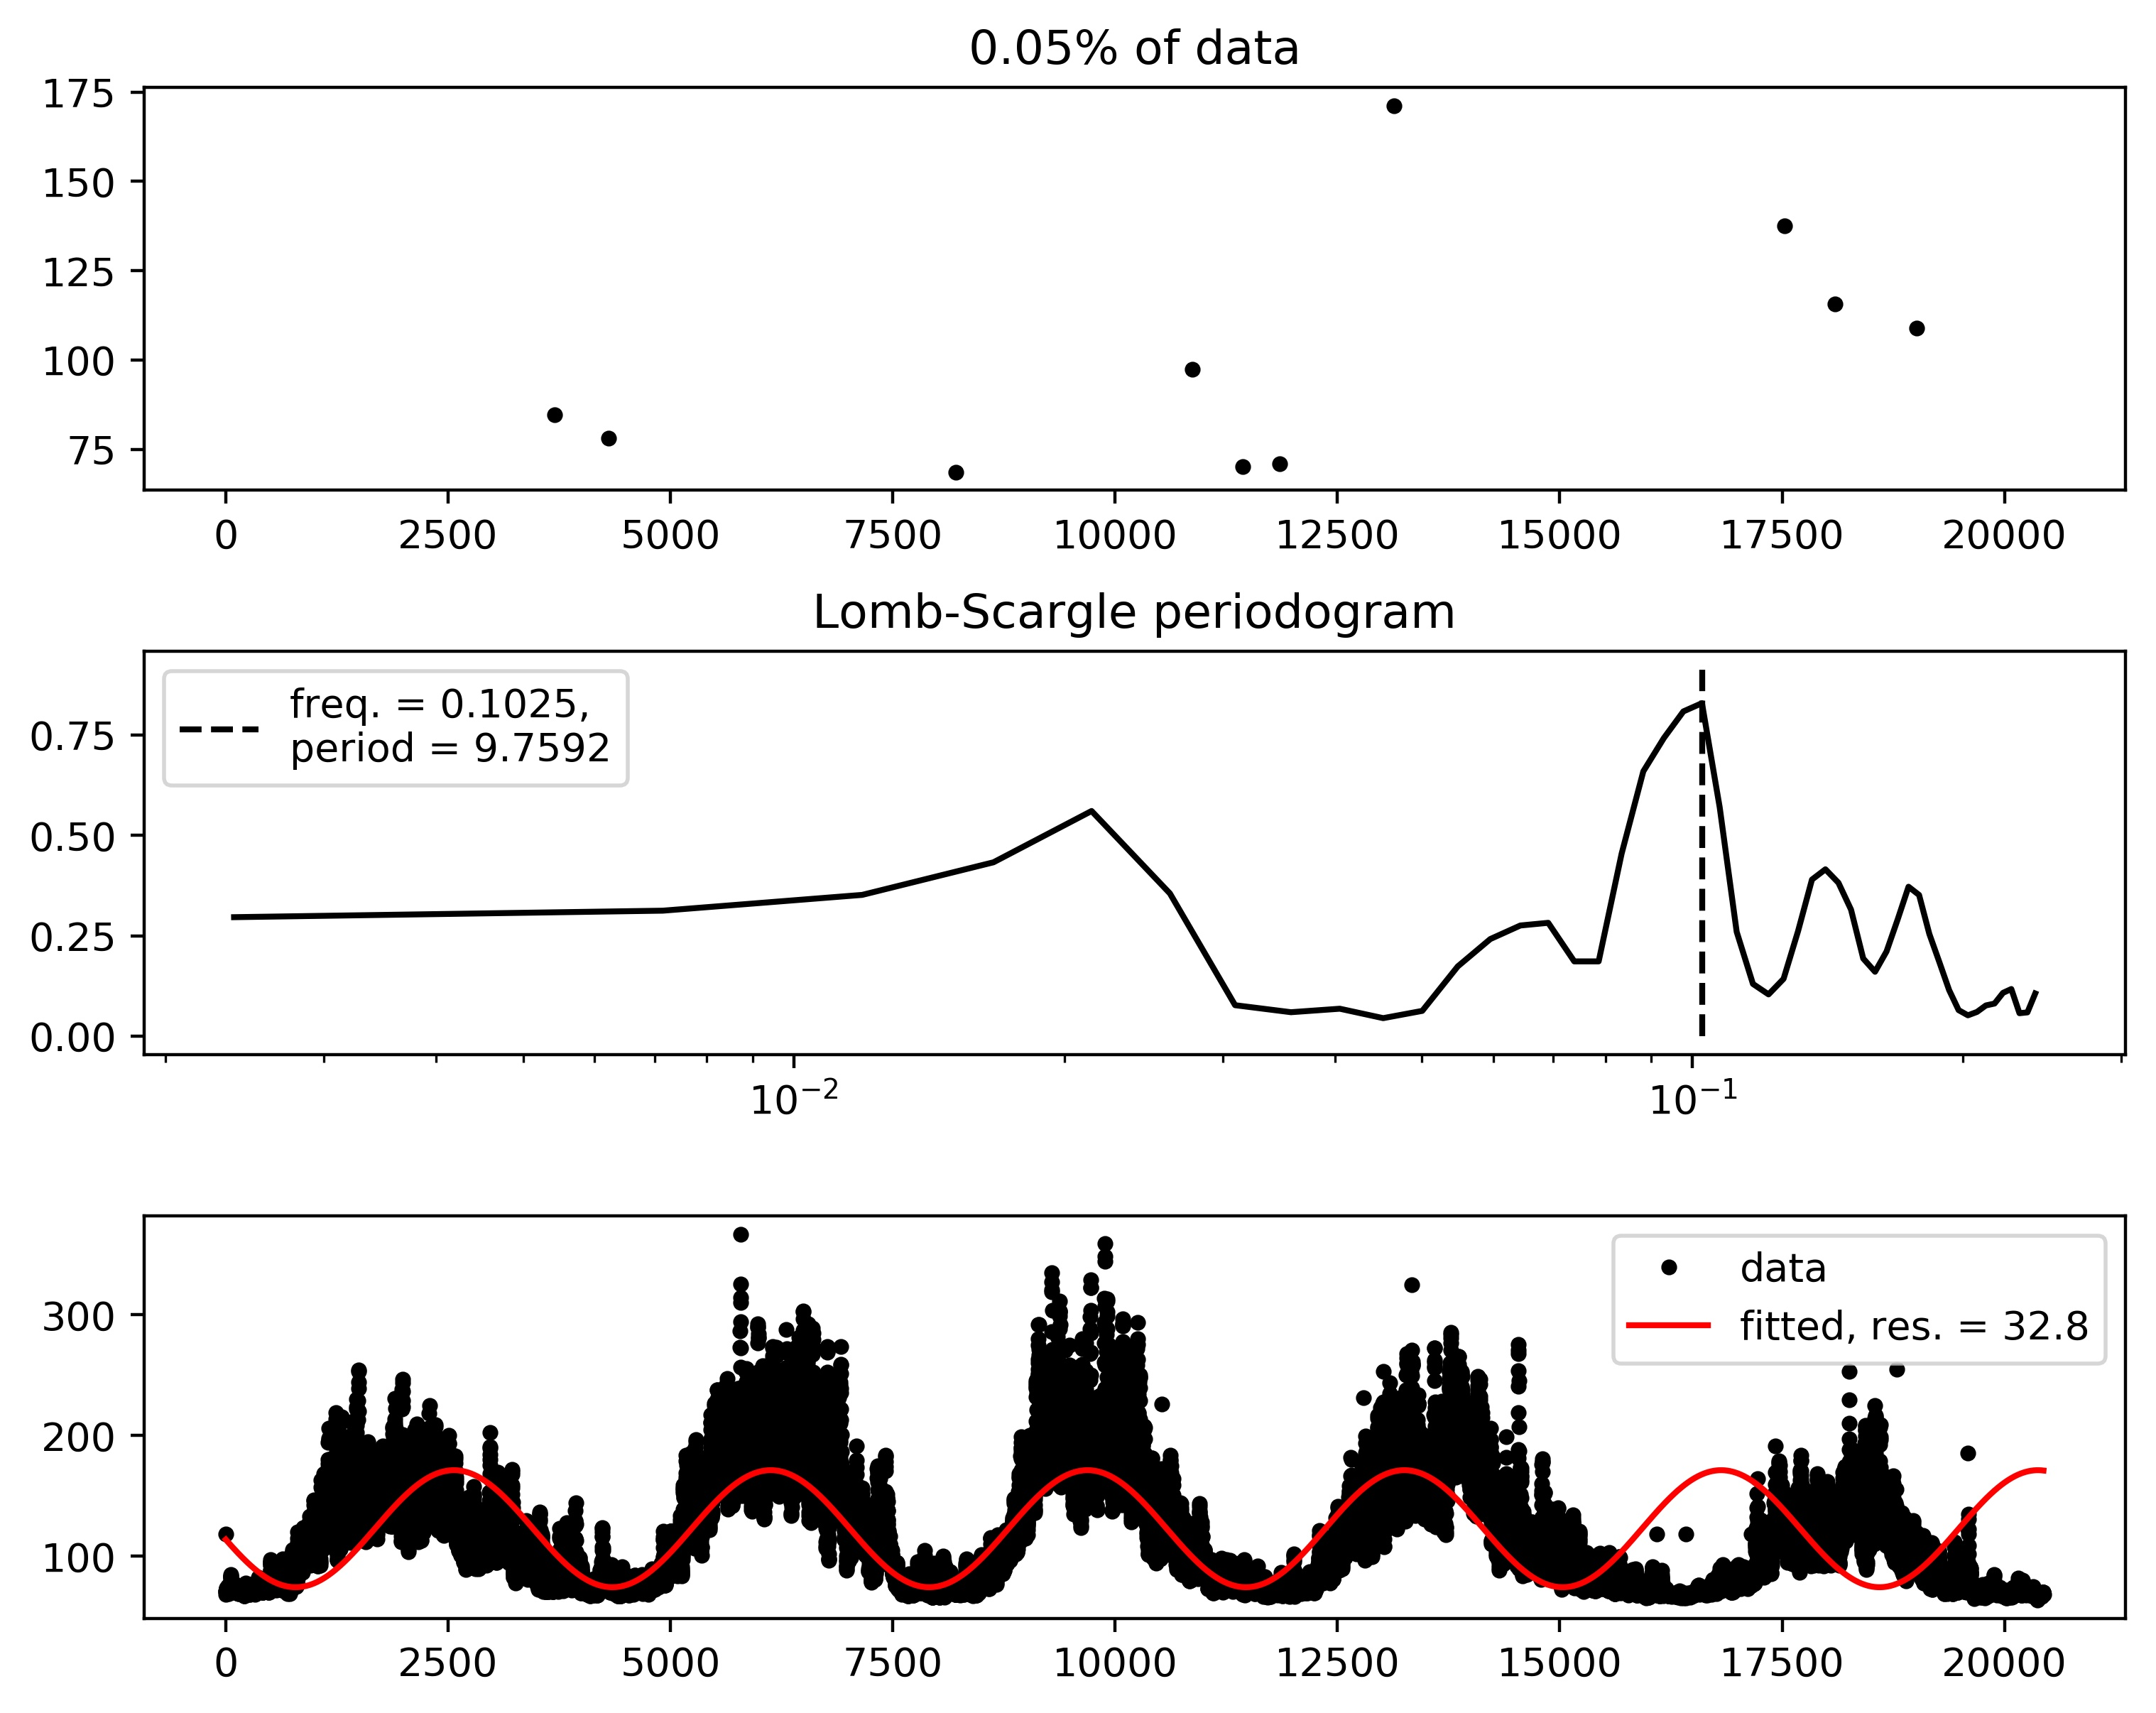
\includegraphics{../scripts/dataset1/periodograms_ny2.0_model1_pg0.9995.jpg}}
	\end{center}
	\vspace{-1mm}	
	\legenda{Aqui o periodograma de Lomb-Scargle apresenta seus picos com baixa resolução (picos espalhados). Ainda assim, a frequência determinada é satisfatória e a senóide resultante se ajusta bem à série, conforme ilustrado pelo plot de baixo.}
	\label{fig:percent0.05}
\end{figure}

\begin{figure}[ht!]
\vspace{-10mm}	
	\caption{Análise com exclusão aleatória até 0.04\% dos dados.}
	\vspace{1mm}	
	\begin{center}
		\resizebox{.8\textwidth}{!}{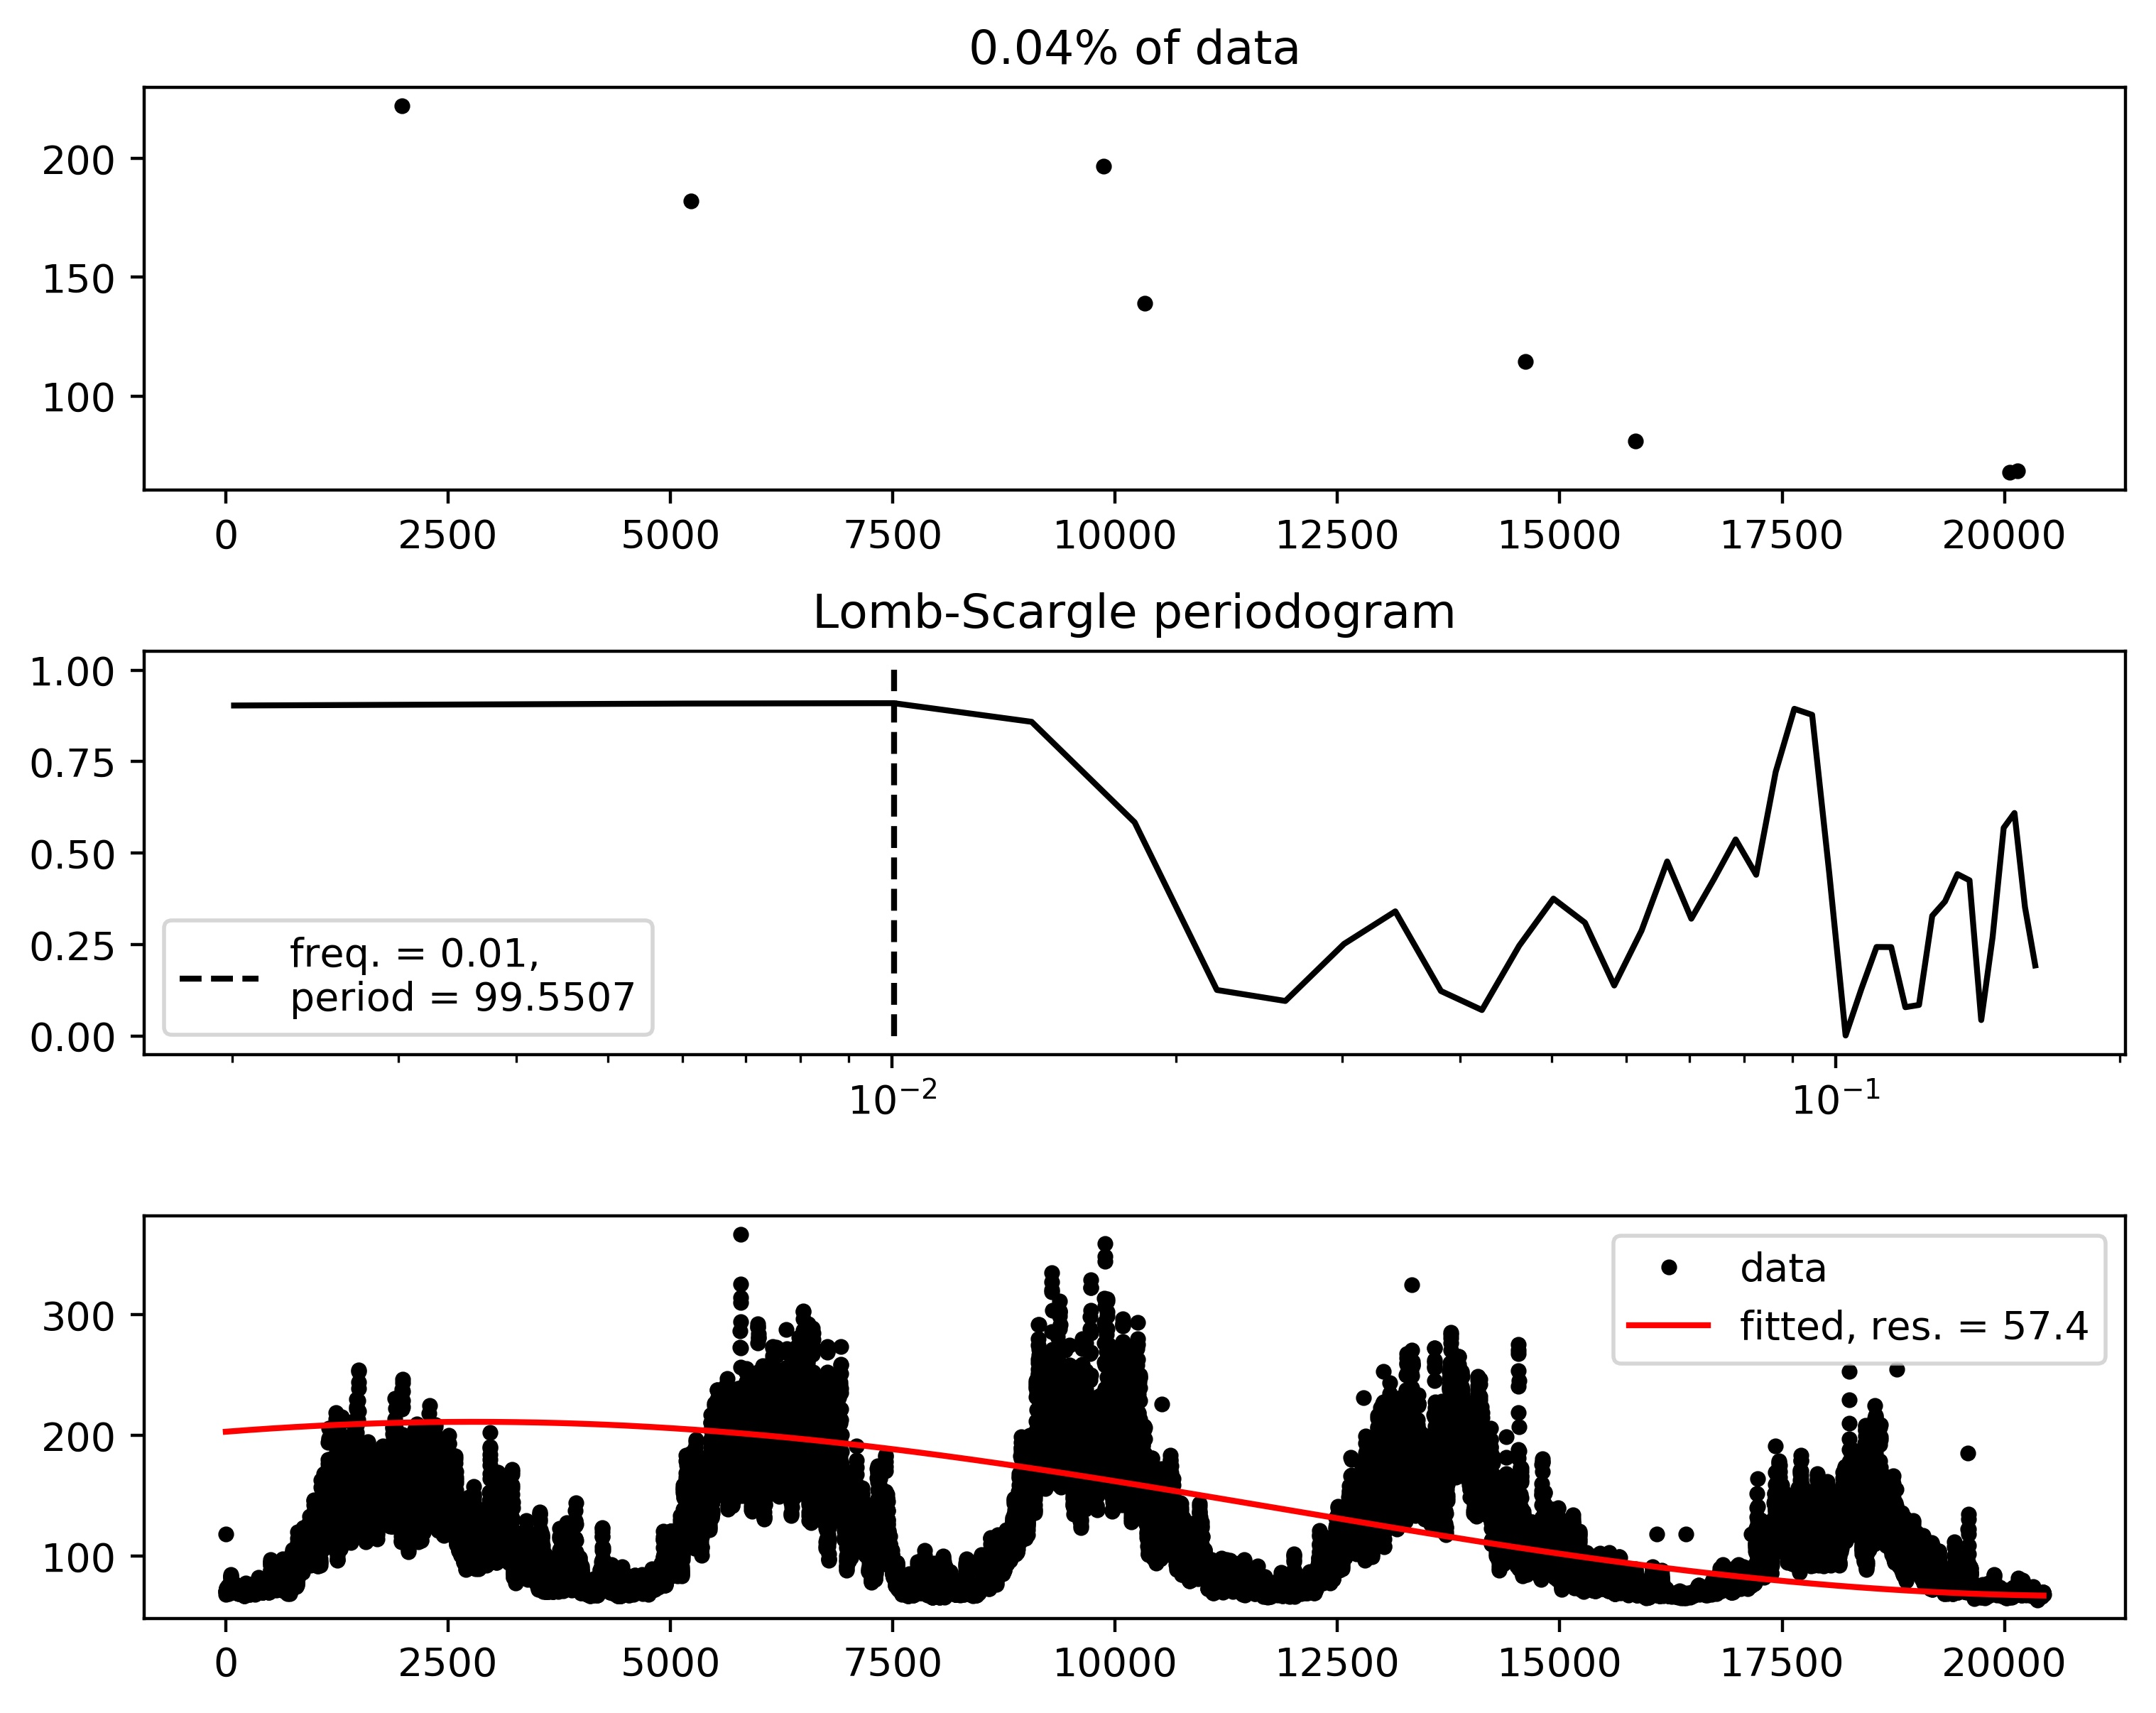
\includegraphics{../scripts/dataset1/periodograms_ny2.0_model1_pg0.9996.jpg}}
	\end{center}
	\vspace{-1mm}	
	\legenda{Neste teste, com 0.04\% dos dados, o periodograma de Lomb-Scargle falhou. A assinatura da série é completamente perdida, e a função ajustada é completamente diferente do esperado.}
	\label{fig:percent0.04}
\end{figure}

\clearpage{}
Para os fins desta discussão, considera-se um bom resultado do \texttt{LombScargle} um periodograma suave, próximo de zero em todas as frequências a não ser pela presença de um pico na frequência conhecida de 0.089 ou próximo desta, e com pouca ou nenhuma frequência espúria. A Figura \ref{fig:percent1} (experimento com 1\% dos dados), se contrastada com as Figuras \ref{fig:4gaps} a \ref{fig:8gaps}, indica que a baixa quantidade de dados não necessariamente afeta a performance da ferramenta. Em outras palavras, o resultado sob as condições da Figura \ref{fig:percent1} foi tão bom ou melhor que sob as condições de todos os testes do cenário anterior. O teste com 0.5\% (Figura \ref{fig:percent0.5}) obteve um resultado tão bom quanto o teste anterior. O teste com 0.1\% dos dados (Figura \ref{fig:percent0.1}) foi particular: mesmo quando o perfil oscilatório (visual) dos dados está totalmente perdido, o uso do \texttt{LombScargle} permitiu recuperar com êxito a característica original do sinal. Abaixo de 0.1\%, assim como durante os testes do cenário anterior, a performance da ferramenta caiu demasiadamente e se tornou igualmente inconsistente para todos os valores. Ou seja, a depender dos dados aleatoriamente excluídos, o resultado da ferramenta era o mesmo com 0.05\% (Figura \ref{fig:percent0.05}) ou 0.04\% (Figura \ref{fig:percent0.04}) dos dados, e estes eram muito piores que os resultados com 0.1\% dos dados ou mais.

 %% 4o capítulo
%\clearpage{}
%%%%%%%%%%%%%%%%%%%%%%%%%%%%%%%%%%%%%%%%%%%%%%%%%%%%%%%%%%%%%%%%%%%%%%%%%%%%%%%
\chapter{CONSIDERAÇÕES FINAIS}

As atividades realizadas no presente trabalho tiveram como objetivo introdução à ferramenta conhecida como periodograma de Lomb-Scargle. Os dados de fluxo solar na faixa de 10.7 cm foram manipulados a fim de simular as condições em que o periodograma de Lomb-Scargle é aplicado: na análise de séries temporais com amostragem aleatória. Os experimentos foram realizados em dois cenários: (1) com $N$ intervalos aleatoriamente distribuídos sobre os dados e de tamanho igual a 10\% do mesmo, e (2) com exclusão aleatória de amostras até $p$\% de amostras restantes. Cinco valores de $N$ e cinco valores de $p$ foram aplicados sobre os dados do fluxo solar, e em seguida seu periodograma produzido com a classe \texttt{LombScargle} do pacote \texttt{astropy} (da linguagem \texttt{Python}).

Os resultados obtidos com a ferramenta empregada foram consistentes na maioria dos testes, indicando robustez da mesma e domínio de seu uso durante a análise. O parâmetro \texttt{nyquist\_factor} empregado foi variado de modo a testar um valor ideal, uma vez que a heurística padrão não permitia enxergar adequadamente a frequência principal na maioria dos testes. Com o valor de 3, o periodograma tinha performance muito ruim na maioria dos testes. A partir deste valor, a ferramenta passou a retornar um pico para a frequência de valor 1, ou seja, um alias persistia nas análises. Para o valor de 2, a ferramenta se tornou consistente e com performance vastamente superior à heurística padrão.

%Com relação a possíveis melhorias na análise, a escolha da melhor frequência foi obtida através da posição do pico nos periodogramas. Esse método pode não ser ideal, pois leakages foram recorrentes durante os testes. Por vezes o pico ocorria em um dos extremos do intervalo de frequência testado pela ferramenta. Um método mais cuidadoso deve ser empregado, ou um teste de diferentes  \texttt{nyquist\_factor} realizados antes da determinação da frequência principal. Além disso, a incerteza das medidas pode ser passada como input à classe \texttt{LombScargle} implementada, o que tornaria a análise ainda mais robusta.

Em resumo, os diferentes efeitos da amostragem foram explorados. Em particular, o efeito de amostragem não uniforme. Sob tal condição, o espectro de potência via FFT não é mais aplicável e o periodograma de Lomb-Scargle se torna a ferramenta ideal. Num pipeline de análise, sua implementação através da classe \texttt{LombScargle} do pacote \texttt{astropy} requer cuidados com a escolha da heurística. Durante os testes aqui realizados, essa ferramenta foi capaz de corretamente identificar o período de $\sim$11 anos do ciclo solar através dos dados de média diária do fluxo F10.7. O ajuste de mínimos quadrados para análise espectral se mostrou robusto na maioria dos cenários testados, e a senóide recuperada se ajustou bem aos dados originais. %Vale ressaltar que a série analisada é não linear, uma vez, durante um ciclo, seu pico cresce mais rapidamente que seu vale decresce.

%Foi tudo ok. Vale ressaltar que esta série é aproximadamente não linear, pois decresce mais rapidamente que cresce. Essa característica não será capturada pelo ajustes de funções senos, exigindo técnicas mais específicas como redes neurais. 

 %% 5o capítulo

%\include{./docs/capitulo6} %% 6o capítulo


%% insira quantos capítulos desejar com o seguinte comando:
%\include{_pasta_do_arquivo_/_meu_arquivo_} %%sem a extensão
%% note que deverá haver um arquivo _meu_arquivo_.tex (com extensão) no diretório _pasta_do_arquivo_

%\include{./docs/conclusao}

%\newpage
%% Bibliografia %% não alterar %% obrigatório %testebib
\bibliography{./bib/referencia} %% aponte para seu arquivo de bibliografia no formato bibtex (p.ex: referencia.bib)


%\include{./docs/glossario} %% insira os termos do glossário no arquivo glossario.tex %% opcional

%\inicioApendice %% opcional, comente esta linha e a seguintes se não houver apendice(s)
%\include{./docs/apendice1} %% insira apendices tal qual capítulos acima


%\inicioAnexo
%\include{./docs/anexo}
%\include{./docs/anexo1}
%\include{./docs/anexo2}

%\inicioIndice
%\include{./docs/contracapa}
\end{document}